 \documentclass[12pt,a4paper]{report}

% ================= PACKAGES =================
\usepackage[utf8]{inputenc}
\usepackage[T1]{fontenc}
\usepackage[french]{babel}
\usepackage{graphicx}
\usepackage{array}
\usepackage{booktabs}
\usepackage{geometry}
\usepackage{setspace}
\usepackage{palatino}
\usepackage[titles]{tocloft}
\usepackage{fancyhdr}
\usepackage{microtype}
\setlength{\headheight}{14.5pt}
\usepackage{longtable}
\usepackage{xcolor} % Pour les couleurs
\usepackage{colortbl} % Pour les couleurs dans les tableaux
% Pour la version alternative :
\usepackage{tikz} % Pour les éléments graphiques
\usepackage{float}
\usepackage{placeins} % Optionnel, pour \FloatBarrier
\usepackage{pdflscape} % Pour les pages en mode paysage

% ================= CONFIGURATION =================
\geometry{margin=2.5cm}
\onehalfspacing

% Configuration des en-têtes et pieds de page
\pagestyle{fancy}
\fancyhf{}
\fancyhead[L]{\nouppercase{\leftmark}}
\fancyhead[R]{\thepage}
\renewcommand{\headrulewidth}{0.5pt}

% Configuration de la table des matières
\renewcommand{\cfttoctitlefont}{\huge\bfseries}
\renewcommand{\contentsname}{Table des Matières}
\renewcommand{\listfigurename}{Table des Figures}
\renewcommand{\listtablename}{Liste des Tableaux}

% Load hyperref last to avoid duplicate destination warnings
\usepackage[hidelinks]{hyperref}

% ================= DOCUMENT =================
\begin{document}

% ================= PAGE DE TITRE =================
% Page de titre sans numéro
\begin{titlepage}
    \centering
    \vspace*{2cm}
    
    {\Huge \textbf{Rapport de Projet de Fin d'Études}}\\[1cm]
    {\LARGE \textbf{Développement d'un CRM Micro-SaaS Haute Performance}}\\[2cm]
    
    {\Large Présenté par :}\\[0.5cm]
    {\Large AmenAllah}\\[1cm]
    
    {\Large Pour l'obtention du diplôme d'ingénieur en}\\[0.5cm]
    {\Large Génie Logiciel}\\[2cm]
    
    {\Large Date : \today}
    
    \vfill
\end{titlepage}

% ================= PAGES PRÉLIMINAIRES =================
% Numérotation en chiffres arabes à partir de 1
\pagenumbering{arabic}
\setcounter{page}{1}

% Dédicace (page 1)
\chapter*{Dédicace}
\addcontentsline{toc}{chapter}{Dédicace}

% Police Times New Roman
\fontfamily{ptm}\selectfont
\linespread{1.0}
\thispagestyle{plain}

% RÉDUIT l'espacement depuis le haut
\vspace*{0.5cm} % Réduit de 1.5cm à 0.5cm

% Ligne horizontale - PLUS PROCHE du texte
\noindent\rule{\textwidth}{2pt}

% Texte principal - IMMÉDIATEMENT après la ligne
\vspace{0.1cm} % Réduit pour tenir sur une page

{\large Je dédie ce travail.}

\vspace{0.2cm} % Réduit pour tenir sur une page

À mon cher père, \textbf{Abdelmajid Mselmi},Parce qu’il a été là, sans faiblir, dans chaque moment important. Ses mots doux résonnent encore aujourd’hui, bien après leur départ. Chaque effort silencieux pèse plus lourd que n’importe quel discours. Ce calme fort, cette présence posée - voilà ce qui m’a porté loin. Rien ne suffit à dire la profondeur de ce lien vrai. Qu’un souffle divin prolonge ses jours, apaise son corps, éclaire sa route.

\vspace{0.2cm} % Réduit pour tenir sur une page

À ma tendre mère, \textbf{Aida Brahem},Chaque mot doux qu'elle offrait portait une force tranquille. Par moments flous, c’est son calme qui tenait debout à ma place. Quand l’ombre gagnait, des phrases simples jaillissaient - toujours au bon moment. Rien n’était exigé, pourtant tout venait. L’épaule silencieuse où poser le poids sans avoir besoin de parler. Même en silence, elle disait assez. Pas de gestes spectaculaires, juste là, jour après jour. Ce genre de constance change la trajectoire sans bruit.

\vspace{0.2cm}

À ma sœur jumelle, \textbf{Amal Mselmi}, À preuve, ce lien fort, cet amour simple entre frères. Difficile d’aligner des phrases assez justes pour dire le respect que j’ai pour lui, surtout après tout ce temps passé côte à côte dans ce parcours universitaire. Parce qu’il était là, toujours.
\vspace{0.2cm}

À mon frère, \textbf{Anis Mselmi},Grâce à lui, chaque étape fut plus claire. Son appui sans faille a porté mes pas durant ce chemin difficile. Par moments, c’est son calme qui parlait le plus fort. Il était là, simplement, quand l’effort semblait trop lourd. Ce projet, aujourd’hui achevé, porte aussi son souffle. Chaque avancée s’est nourrie de sa confiance tranquille.

\vspace{0.2cm}

Parce qu’ils étaient là sans poser de questions, à ceux que je croyais connaître – puisqu’on a tout fait ensemble, même ce truc dans la cour après minuit. Un silence parfois remplace un merci. Leur rire résonne encore ici. Chaque faux pas devient une trace quand on avance avec eux. Rien n’était prévu, mais tout restera.

\vspace{0.5cm} % Réduit pour tenir sur une page

\hfill{\itshape AmenAllah}

% La police Times est déjà active, pas besoin de changer
\clearpage

% Remerciements (page 2)
\chapter*{Remerciements}
\addcontentsline{toc}{chapter}{Remerciements}

% Police Times New Roman
\fontfamily{ptm}\selectfont
\linespread{1.0}

% Ligne horizontale
\noindent\rule{\textwidth}{2pt}

% Texte principal
\vspace{0.3cm}

{\large Je tiens à exprimer ma profonde gratitude.}

\vspace{0.3cm}

Un grand merci à mon professeur encadrant, \textbf{M. Alhoussem Chtioui}, pour le temps qu’il a consacré avec tant de soin à chaque étape de ce projet. Grâce à lui, les moments difficiles sont devenus plus clairs, car il savait toujours poser les bonnes questions au moment juste. Ce n’est pas seulement son savoir qui a compté, mais surtout sa manière calme et précise de guider sans imposer. Chaque rencontre ouvrait une nouvelle direction, jamais en ligne droite, souvent par des chemins détournés mais utiles. Il ne donnait pas les réponses toutes faites, plutôt des indices discrets qui poussaient à chercher encore. Sa façon de travailler m’a appris à mieux organiser mes idées, à vérifier deux fois avant d’affirmer. Loin des discours vides, il insistait sur l’exactitude, même dans les détails invisibles. Sans cette présence attentive, ce mémoire aurait pris une autre forme, moins solide, certainement moins aboutie. Ce que j’ai gagné va bien au-delà du sujet traité - c’est une manière différente de penser, plus exigeante, plus lucide.

\vspace{0.3cm}

Un grand merci à mon tuteur en entreprise, \textbf{M. Amine Ben Slimene}, pour son aide constante, sa grande écoute et ses indications claires durant tout le stage. Ce n’est pas tous les jours qu’on croise quelqu’un qui allie savoir-faire technique et vue d’ensemble comme il l’a fait. Grâce à lui, j’ai vu comment fonctionnent vraiment les choses derrière un projet CRM. Les idées abstraites vues en cours prennent soudain sens quand on les met face aux situations du terrain. Chaque discussion avec lui ouvrait une nouvelle porte sur ce que signifie travailler dans ce secteur. L’écart entre la salle de classe et l’usine se rétrécit vite quand on est guidé ainsi. Sa manière calme mais précise de répondre m’a évité bien des détours inutiles. Jamais je n’aurais imaginé voir autant de détails entrer en jeu dans chaque décision. Il ne donnait pas simplement des réponses, il montrait où chercher. Tout cela change profondément la façon dont je vois maintenant certaines étapes du travail. Sans cette présence attentive, beaucoup serait resté flou. La théorie garde toujours un goût partiel tant qu’elle ne touche pas la pratique. C’est exactement ce qu’il a permis : rapprocher deux mondes souvent séparés.

\vspace{0.3cm}

Un grand merci à \textbf{M. Firas Beguiga}, toujours présent, qui a guidé chaque étape avec attention. Grâce à lui, les idées ont pris forme, pas à pas. Ses remarques précises ont souvent ouvert de nouvelles pistes. Quand les difficultés techniques surgissaient, il prenait le temps d’en parler, calmement. Chaque échange apportait une pièce manquante au puzzle. Ce sont ses propositions simples mais justes qui ont fait avancer les choses. Même quand la pression montait, sa clarté d’esprit restait intacte. Loin des grandes phrases, ses interventions ciblées ont marqué toute la durée du projet. Sans ces moments d’échanges francs, bien des améliorations n’auraient pas eu lieu. Son regard acéré sur les zones fragiles a évité bien des détours. À plusieurs reprises, c’est par son calme que la direction s’est redressée. Ce travail en porte forcément la trace.

\vspace{0.3cm}

Merci beaucoup aux enseignants de l’\textbf{ISSAT de Sousse} - leur façon nette d’expliquer tient une grande place dedans. Souvent présents quand on avait besoin, ils ont donné les outils juste nécessaires pendant toute la formation d'ingénieur. Leur rigueur au quotidien comptait énormément. Chaque détail vu en cours s’est révélé utile plus tard. Ce qu’ils transmettent va bien au-delà des programmes. Sans vraiment y penser sur le moment, chacune de leurs attitudes a aidé à construire un socle solide, prêt à servir maintenant.

\vspace{0.3cm}
Merci beaucoup à l’équipe technique de \textbf{VisioAd}, qui a tout de suite ouvert la porte. Dès le départ, leur façon de s’entraider simplifiait tout. Quand un problème surgissait, ils étaient là sans attendre. Grâce à eux, avancer était naturel. Chaque échange donnait une idée utile, pas juste des mots en trop. Un frisson court le long de l'instant, reste accroché. Pas besoin de chercher ailleurs pour sentir ce poids léger entre les mains.

\vspace{0.3cm}

Voilà ceux qui rendent les choses vraies, en lisant mot après mot, sans courir. Pas besoin de dire merci : leurs yeux restent là, tranquilles, fixés. Sans ça, tout s’effondrerait, lentement, comme du papier mouillé. Un souffle retenu entre deux phrases dit autant qu’un cri parfois. Ce moment volé au reste pèse lourd, même si personne ne le mesure.

\vspace{0.5cm}

\hfill{\itshape AmenAllah}

% Retour à la configuration normale
\linespread{1.0}
\clearpage

% Liste des acronymes (page 3)
\chapter*{Liste des Acronymes}
\addcontentsline{toc}{chapter}{Liste des Acronymes}

% Style pour ce chapitre
\thispagestyle{fancy}
\pagestyle{fancy}

% En-tête stylisé
\begin{center}
\vspace*{1cm}
{\Large\bfseries Liste des Acronymes}\\[0.5cm]
{\small Les acronymes utilisés dans ce document sont définis ci-dessous par ordre alphabétique.}\\[1cm]
\end{center}

% Ligne décorative
\noindent\rule{\textwidth}{1pt}\\[0.5cm]

% Tableau avec design amélioré
\begin{longtable}{p{3.5cm}>{\raggedright\arraybackslash}p{10.5cm}}
\rowcolor{gray!10} % Fond gris clair pour l'en-tête
\textbf{\large Acronyme} & \textbf{\large Signification et Description} \\
\endfirsthead

\rowcolor{gray!10}
\textbf{\large Acronyme} & \textbf{\large Signification et Description} \\
\endhead

\hline
\endfoot

\hline
\multicolumn{2}{c}{\small \textit{Suite de la liste des acronymes à la page suivante}} \\
\endlastfoot

% Contenu du tableau avec meilleure présentation
\textbf{2TUP} & \textbf{2 Tracks Unified Process} (Processus Unifié à Deux Voies) - Méthodologie de développement séparant les aspects fonctionnels et techniques \\
\hline
\textbf{API} & \textbf{Application Programming Interface} (Interface de Programmation d'Application) - Ensemble de règles permettant à des applications de communiquer entre elles \\
\hline
\textbf{APIGEE} & \textbf{API Gateway Enterprise Edition} - Plateforme de gestion d'API développée par Google \\
\hline
\textbf{AWS} & \textbf{Amazon Web Services} - Plateforme de cloud computing d'Amazon \\
\hline
\textbf{BaaS} & \textbf{Backend-as-a-Service} (Backend en tant que Service) - Modèle de cloud computing externalisant les services backend \\
\hline
\textbf{CI/CD} & \textbf{Continuous Integration and Continuous Delivery/Deployment} (Intégration et Livraison/Déploiement Continus) - Pratiques de développement logiciel \\
\hline
\textbf{DAO} & \textbf{Data Access Object} (Objet d'Accès aux Données) - Patron de conception pour l'abstraction de l'accès aux données \\
\hline
\textbf{DTO} & \textbf{Data Transfer Object} (Objet de Transfert de Données) - Patron de conception pour le transfert de données entre les couches \\
\hline
\textbf{FaaS} & \textbf{Function-as-a-Service} (Fonction en tant que Service) - Modèle de cloud computing pour l'exécution de fonctions sans serveur \\
\hline
\textbf{IaC} & \textbf{Infrastructure as Code} (Infrastructure en tant que Code) - Gestion de l'infrastructure via des fichiers de configuration \\
\hline
\textbf{IDMS} & \textbf{Identity Management System} (Système de Gestion d'Identités) - Système pour la gestion des identités utilisateurs \\
\hline
\textbf{JWT} & \textbf{Json Web Token} - Standard pour la création de jetons d'authentification \\
\hline
\textbf{MVC} & \textbf{Model-View-Controller} (Modèle-Vue-Contrôleur) - Patron architectural pour les interfaces utilisateur \\
\hline
\textbf{MVP} & \textbf{Model-View-Presenter} (Modèle-Vue-Présentateur) - Patron architectural dérivé du MVC \\
\hline
\textbf{RUP} & \textbf{Rational Unified Process} - Processus de développement logiciel itératif \\
\hline
\textbf{SDK} & \textbf{Software Development Kit} (Kit de Développement Logiciel) - Ensemble d'outils pour développer des applications \\
\hline
\textbf{SCRUM} & \textbf{Méthodologie Agile de gestion de projet} - Cadre de travail itératif et incrémental \\
\hline
\textbf{SSL} & \textbf{Secure Sockets Layer} - Protocole de sécurisation des communications sur Internet \\
\hline
\textbf{UP} & \textbf{Unified Process} - Processus de développement logiciel unifié \\
\hline
\textbf{VPC} & \textbf{Virtual Private Cloud} (Cloud Privé Virtuel) - Réseau virtuel isolé dans le cloud \\
\hline
\textbf{XP} & \textbf{eXtreme Programming} - Méthodologie de développement logiciel agile \\

\end{longtable}

% Note en bas de page
\vspace{0.5cm}
\begin{center}
\fbox{\parbox{0.9\textwidth}{
\small\textit{Note : Les acronymes sont présentés par ordre alphabétique pour faciliter la recherche. Chaque entrée inclut l'acronyme en gras, sa signification complète et une brève description de son utilisation dans le contexte de ce projet.}
}}
\end{center}
\clearpage

% ================= TABLES =================
% Table des matières (page 4)
\tableofcontents
\clearpage

% Table des figures (page 5)
\listoffigures
\clearpage

% Liste des tableaux (page 6)
\listoftables
\clearpage

% ================= CONTENU PRINCIPAL =================
% La numérotation continue automatiquement (page 7, 8, 9, ...)

% Introduction générale (page 7)
\chapter*{Introduction Générale}
\addcontentsline{toc}{chapter}{Introduction Générale}

Quand la pression monte dans le monde du travail, suivre sa clientèle devient central. Surtout en B2B. Ce n’est plus seulement un carnet d’adresses électronique. Ces systèmes touchent maintenant chaque moment de la vente. L’acheteur s’y sent mieux accompagné. Les chiffres finaux montrent souvent une amélioration. Pourtant, en regardant bien les options offertes, on tombe sur un même problème. Les petites équipes sont régulièrement mises de côté. Trop complexes parfois. Parfois mal conçus. Le fonctionnement paraît brouillon. Le prix fait peur. La vitesse chute avec beaucoup de données. L’ajustement aux habitudes locales est rarement fluide.

\vspace{0.5cm}

Ça commence par une idée simple. Un truc monté à partir de presque rien. Ce projet s'inscrit ici, non pas en cassant tout, mais en suivant le courant. Le but ? Quelques mots suffisent. Créer un CRM micro-SaaS solide, fait pour les petites équipes commerciales ciblant les pros. Depuis un moment déjà, on voit ce trou. Rien d’offert qui soit léger, vif, sans frais cachés, tout en restant puissant. Ce projet vise quelque chose de précis. Il veut mélanger puissance calme des grands outils et agilité des applications modernes. Ici, une interrogation monte. Comment créer un CRM fiable, qui ne bloque pas quand l’équipe grossit ? Un système ouvert aux petites équipes commerciales. Quelque chose de rapide même sous charge. Sans sacrifier le confort d’utilisation chaque jour.

\vspace{0.5cm}

C’est avant tout un CRM léger fait pour les petites équipes en B2B. Son cœur fonctionne fort, prêt à monter en puissance si besoin. Chaque détail tient la route, surtout le suivi des contacts qui glisse sans accroc. Pas de fouillis partout, l’écran montre juste l’essentiel. Derrière ce calme visuel se cache une machine bien réglée. Des transferts fluides circulent d’un système à l’autre grâce à des outils d’import modulables. En temps réel, chaque modification apparaît dès qu’elle est enregistrée. La sécurité veille en silence durant toutes les phases actives. C’est là un projet imposé dans le cadre universitaire pour clore le parcours ingénieur logiciel. Ce travail a pris forme sur une demi-année au sein de VisioAd, accompli en fin de cursus.

\vspace{0.5cm}

Tout débute comme ça. Un aperçu posé dès l'entrée pour donner une direction claire à ce qui suit. Le texte progresse étape après étape, sans se précipiter. Chaque partie examine un angle nouveau - d’abord le cadre du projet, ensuite les besoins repérés, puis une feuille de route réaliste, la phase d’exécution, enfin une évaluation globale avec quelques perspectives envisageables. Le départ se fait depuis ce qui existe déjà. Cela permet de s’appuyer sur des faits tangibles. Petit à petit, on y voit plus net dans les ressorts techniques, humains et fonctionnels liés à notre CRM Micro-SaaS.
\clearpage

% Chapitre 1 (page 8)
\chapter{Cadre du projet}

\section{Introduction}
Au début de ce chapitre, le contexte global du projet est posé. On part avec une présentation de l’organisme d’accueil, suivi par ses prestations ainsi que les outils technologiques utilisés. Plutôt que de rester vague, on examine ici comment notre approche se distingue des systèmes préexistants. Petit à petit, la manière choisie pour concevoir le système prend forme. L’intention ? Offrir un tour complet dès le départ : comprendre qui accueille, voir ce qui existe déjà, puis cerner précisément les attentes techniques comme celles hors technique.

\FloatBarrier % Force toutes les images précédentes à être placées
\section{Contexte général du projet}

\subsection{Cadre du projet}
Ce stage donne une chance rare d’aller plus loin que les cours, tout en mettant les pieds dans la réalité du travail en informatique. Pour valider notre formation d’ingénieur en Génie Logiciel, on a rejoint l’équipe de VisioAd. L'idée ? Créer un outil utile, pas juste théorique : une appli CRM appelée « W261 - CRM Micro-SaaS », pensée pour des commerciaux B2B. Elle doit surtout tenir la route quand le volume monte - rapide, souple, bien construite.

\subsection{Présentation de la société d'accueil : VisioAd}
VisioAd est une entreprise innovante spécialisée dans le développement de solutions digitales pour le marketing et la gestion commerciale. Fondée en 2021, elle accompagne les entreprises dans leur transformation numérique grâce à des outils performants d'analyse de données, d'automatisation marketing et de gestion de campagnes publicitaires.

\begin{figure}[!htbp]
    \centering
    
\includegraphics[width=0.7\textwidth,height=0.35\textheight,keepaspectratio]{images/logo-visioad.jpg}
    \caption{Logo de VisioAd}
    \label{fig:logo-visioad}
\end{figure}
\FloatBarrier % Force cette image à être placée ici

VisioAd opère à l'échelle internationale avec des bureaux en Europe et en Amérique du Nord. L'entreprise valorise l'innovation, la qualité technique et l'expérience utilisateur, ce qui en fait un partenaire idéal pour le développement d'un CRM moderne.

\subsubsection{Services}
VisioAd offre une gamme de services adaptés aux besoins numériques des entreprises :
\begin{itemize}
    \item \textbf{Développement d'applications sur mesure} : solutions web et mobiles.
    \item \textbf{Automatisation marketing} : outils de gestion de campagnes et d'analyse comportementale.
    \item \textbf{Business Intelligence} : tableaux de bord interactifs et rapports personnalisés.
    \item \textbf{Conseil en transformation numérique} : accompagnement stratégique et technique.
\end{itemize}

\subsubsection{Technologies adoptées}
VisioAd utilise un stack technologique moderne et varié :
\begin{itemize}
    \item \textbf{Front-end} : React, Next.js, TypeScript, Tailwind CSS
    \item \textbf{Back-end} : Node.js, NestJS, Python, Go
    \item \textbf{Bases de données} : PostgreSQL, MongoDB, Redis
    \item \textbf{Cloud \& DevOps} : AWS, Docker, Kubernetes, CI/CD (GitHub Actions)
    \item \textbf{Analytics} : Tableau, Power BI, intégrations API
\end{itemize}

\FloatBarrier
\section{Idée émergeante et étude de l'existant}

\subsection{Idée émergeante}
Consciente des défis rencontrés par les petites et moyennes équipes B2B dans la gestion de leurs leads et pipelines, VisioAd a initié le développement d'un CRM léger, performant et facile à prendre en main. L'objectif est de combler le fossé entre les solutions CRM complexes et coûteuses et les outils basiques qui manquent de fonctionnalités avancées.

\begin{figure}[!htbp]
    \centering
    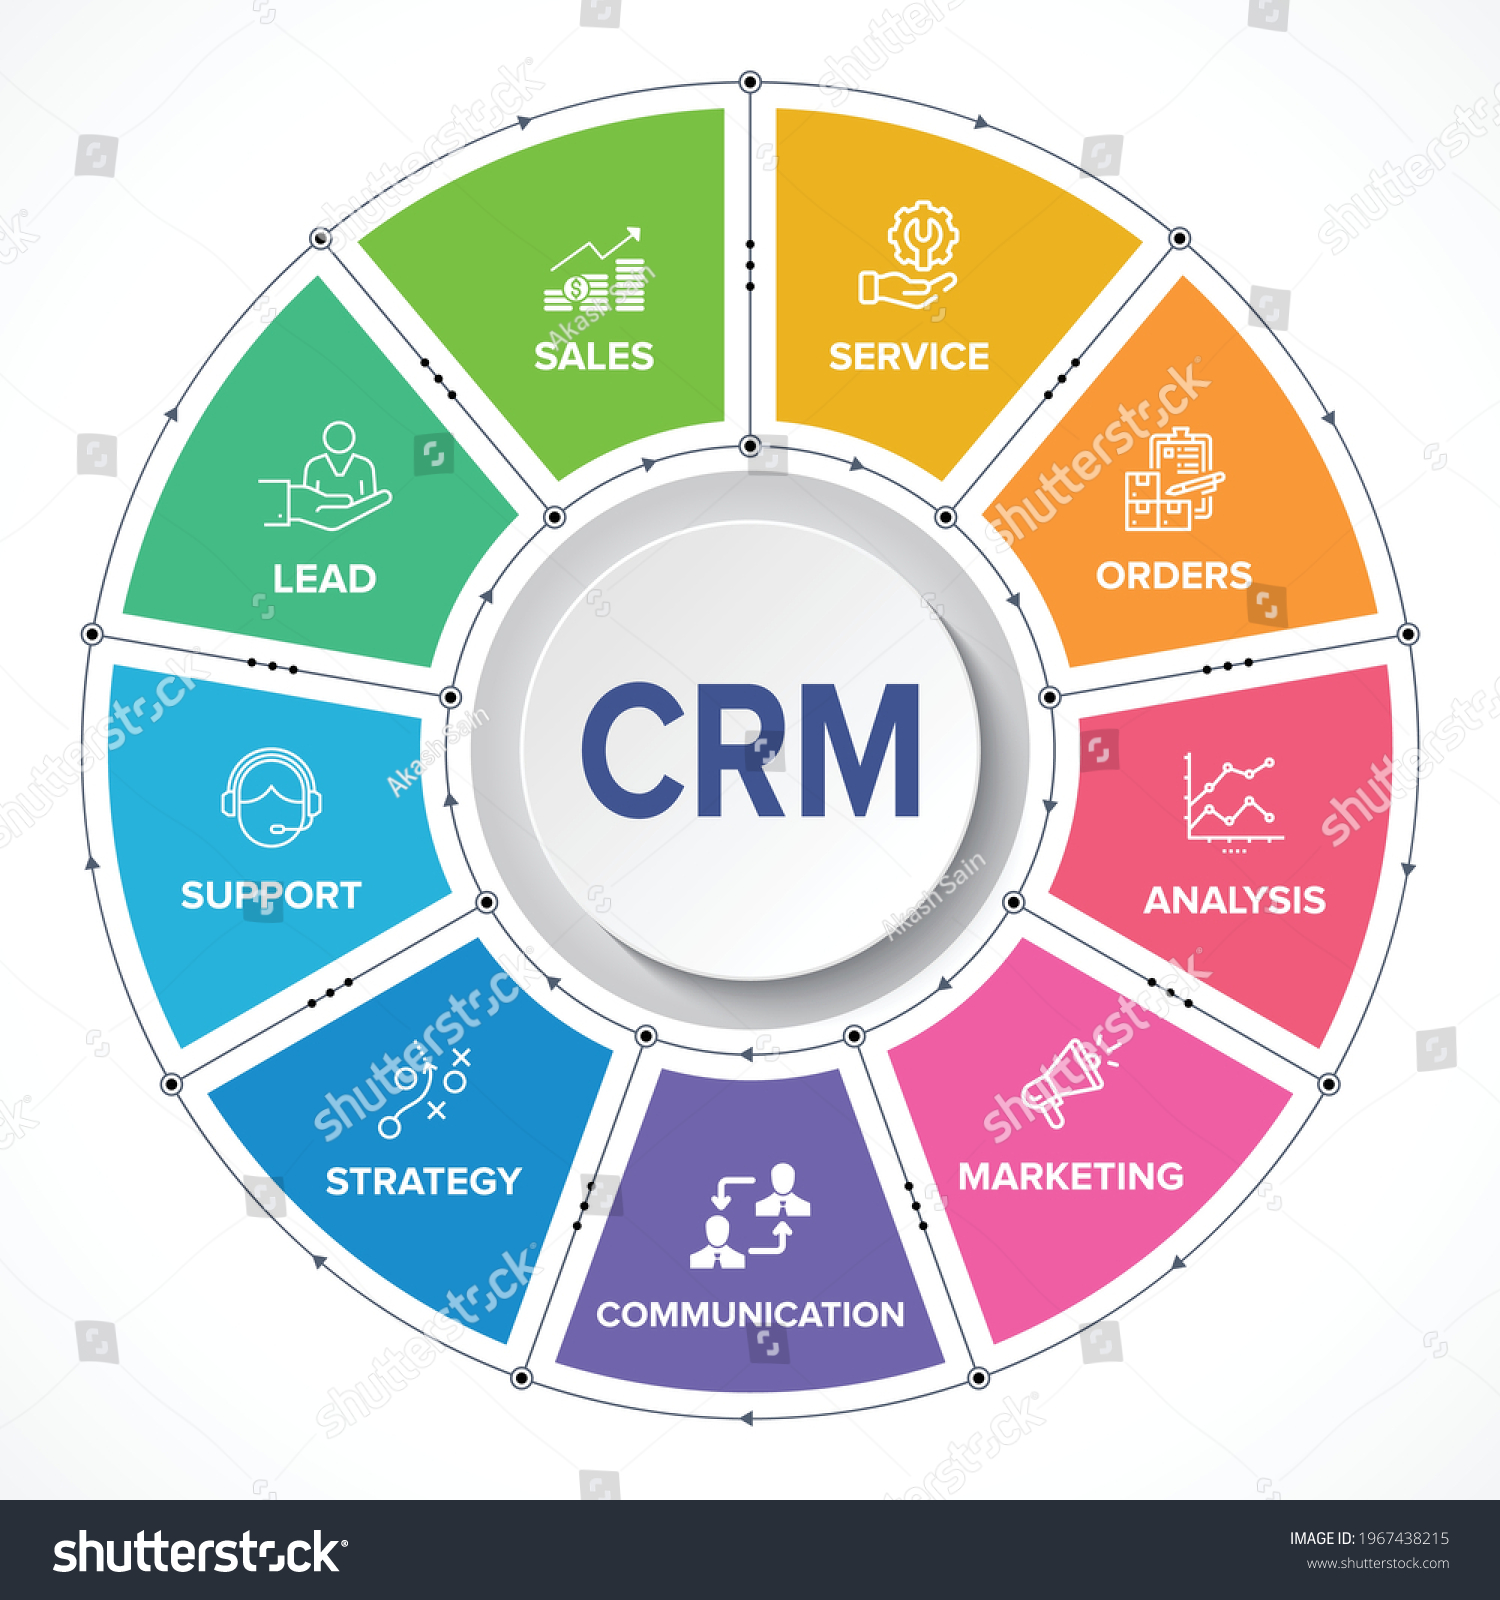
\includegraphics[width=\textwidth,height=0.82\textheight,keepaspectratio]{images/schema-crm-concept.jpg}
    \caption{Architecture conceptuelle du CRM}
    \label{fig:schema-crm}
\end{figure}
\FloatBarrier

\subsection{Analyse comparative des CRM existants}
Une analyse approfondie des trois principales solutions CRM du marché a été réalisée pour identifier leurs forces et faiblesses, et ainsi mieux positionner notre solution.

\subsubsection{Salesforce CRM}
Salesforce est la solution CRM leader du marché, offrant une plateforme complète pour les grandes entreprises.

\begin{figure}[!htbp]
    \centering
    
\includegraphics[width=0.8\textwidth,height=0.45\textheight,keepaspectratio]{images/Salesforce Logo.jpg}
    \caption{Interface de Salesforce CRM}
    \label{fig:salesforce}
\end{figure}
\FloatBarrier

\textbf{Avantages :}
\begin{itemize}
    \item Fonctionnalités très complètes
    \item Écosystème d'applications étendu
    \item intégrations avec de nombreuses plateformes
\end{itemize}

\textbf{Limites :}
\begin{itemize}
    \item Coût très élevé
    \item Complexité de configuration
    \item Surdimensionné pour les petites équipes
\end{itemize}

\textbf{Avantage de notre solution :} Notre CRM offre une alternative abordable et simplifiée, spécialement conçue pour les petites équipes B2B, avec une courbe d'apprentissage réduite.

\subsubsection{HubSpot CRM}
HubSpot propose une solution CRM gratuite avec des options payantes pour les fonctionnalités avancées.

\begin{figure}[!htbp]
    \centering
    
\includegraphics[width=0.8\textwidth,height=0.45\textheight,keepaspectratio]{images/HubSpot-Logo.png}
    \caption{Interface de HubSpot CRM}
    \label{fig:hubspot}
\end{figure}
\FloatBarrier

\textbf{Avantages :}
\begin{itemize}
    \item Version gratuite disponible
    \item Interface utilisateur intuitive
    \item Bonnes intégrations marketing
\end{itemize}

\textbf{Limites :}
\begin{itemize}
    \item Fonctionnalités limitées dans la version gratuite
    \item Personnalisation restreinte
    \item Performances moyennes avec grands volumes
\end{itemize}

\textbf{Avantage de notre solution :} Notre CRM offre une personnalisation complète sans limitations artificielles, avec des performances optimisées pour traiter des milliers de leads sans ralentissement.

\subsubsection{Zoho CRM}
Zoho CRM est une solution flexible adaptée aux entreprises de différentes tailles.

\begin{figure}[!htbp]
    \centering
    
\includegraphics[width=0.8\textwidth,height=0.45\textheight,keepaspectratio]{images/zoho-logo-512.png}
    \caption{Interface de Zoho CRM}
    \label{fig:zoho}
\end{figure}
\FloatBarrier

\textbf{Avantages :}
\begin{itemize}
    \item Coût raisonnable
    \item Bonne personnalisation
    \item Suite d'outils intégrés
\end{itemize}

\textbf{Limites :}
\begin{itemize}
    \item Interface parfois complexe
    \item Performances limitées pour les grands volumes
    \item Expérience utilisateur inégale
\end{itemize}

\textbf{Avantage de notre solution :} Notre CRM utilise une architecture moderne avec virtualisation des données, garantissant une interface fluide même avec 10 000+ leads, et une expérience utilisateur cohérente.

\subsection{Tableau comparatif synthétique}

\begin{table}[!htbp]
\centering
\caption{Comparaison des CRM existants avec notre solution}
\label{tab:comparaison-crm}
\begin{tabular}{|p{3cm}|p{2.5cm}|p{2.5cm}|p{2.5cm}|p{2.5cm}|}
\hline
\textbf{Critère} & \textbf{Salesforce} & \textbf{HubSpot} & \textbf{Zoho} & \textbf{Notre CRM} \\
\hline
Coût & Très élevé & Modéré/Gratuit & Raisonnable & Abordable \\
\hline
Complexité & Élevée & Moyenne & Moyenne-élevée & Faible \\
\hline
Personnalisation & Avancée & Limitée & Bonne & Complète \\
\hline
Performance grands volumes & Bonne & Moyenne & Limitée & Excellente \\
\hline
Interface & Professionnelle & Intuitive & Inégale & Moderne/Fluide \\
\hline
Spécialisation B2B & Générale & Marketing & Générale & Spécifique B2B \\
\hline
\end{tabular}
\end{table}
\FloatBarrier

\begin{figure}[!htbp]
    \centering
    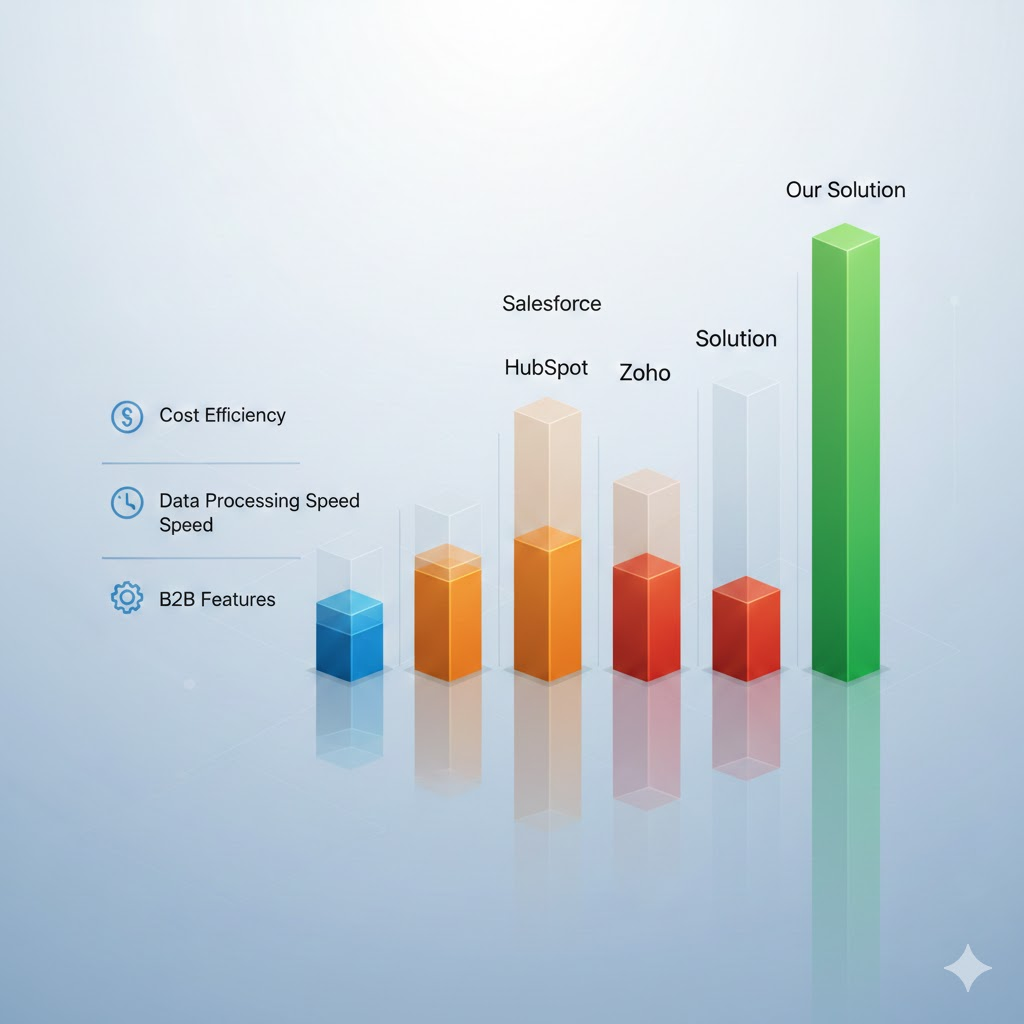
\includegraphics[width=\textwidth,height=0.82\textheight,keepaspectratio]{images/comparaison.jpg}
    \caption{Visualisation comparative des différents CRM}
    \label{fig:comparaison-graphique}
\end{figure}
\FloatBarrier

\subsection{Critique de l'existant}

\subsubsection{Critique du système actuel}
Les solutions CRM actuelles présentent plusieurs limites :
\begin{itemize}
    \item Complexité de configuration et de déploiement.
    \item Coût élevé pour les petites équipes.
    \item Performances dégradées avec de grands volumes de données.
    \item Manque de personnalisation fine pour les workflows B2B.
\end{itemize}

\subsubsection{État de l'art}
Pour proposer une solution compétitive, nous avons étudié des approches modernes de gestion de données volumineuses et d'optimisation d'interface, notamment :
\begin{itemize}
    \item Virtualisation des tableaux de données (TanStack Table).
    \item Architecture serverless et microservices.
    \item Traitement par lots (batch processing) pour l'import CSV.
\end{itemize}

\begin{figure}[!htbp]
    \centering
    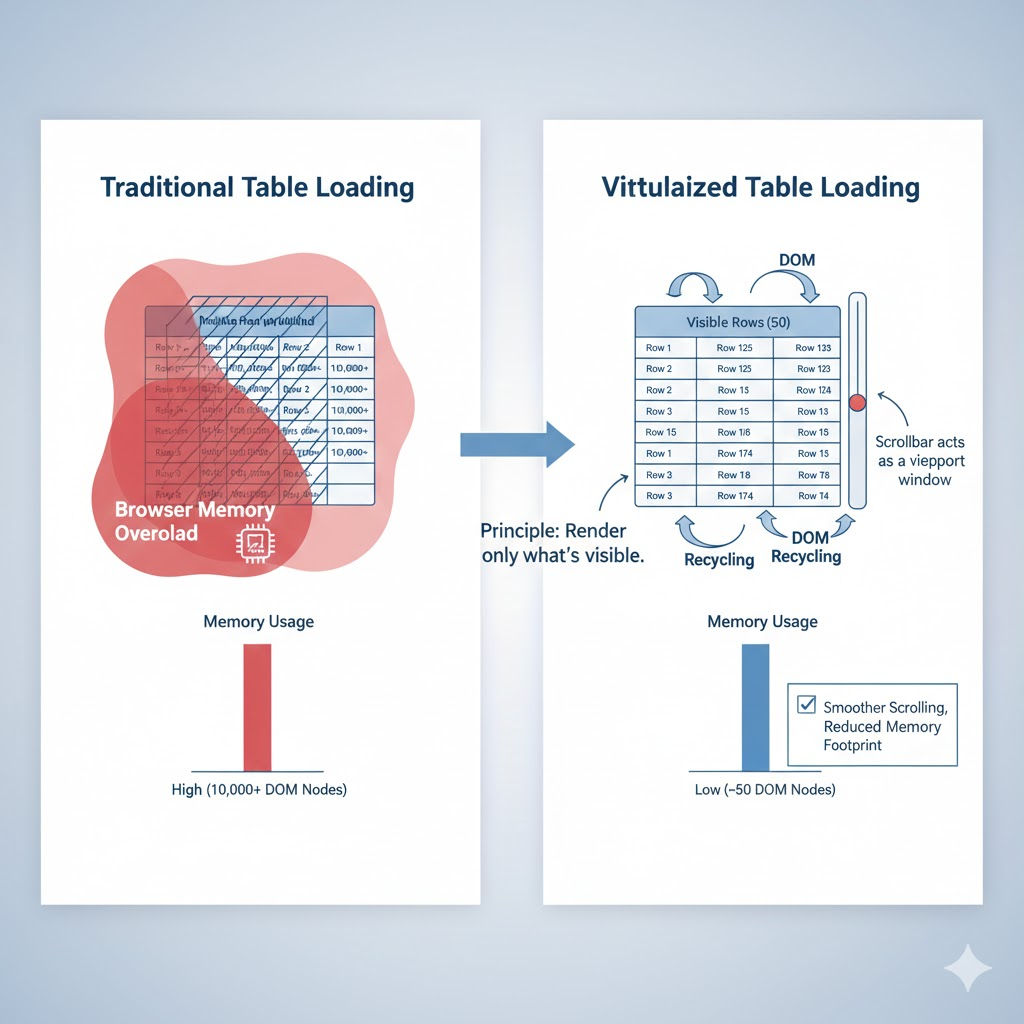
\includegraphics[width=\textwidth,height=0.82\textheight,keepaspectratio]{images/etat.jpg}
    \caption{Principe de virtualisation dans les interfaces data-grid}
    \label{fig:virtualisation}
\end{figure}
\FloatBarrier

\subsection{Solution proposée}
Nous proposons un CRM Micro-SaaS axé sur :
\begin{itemize}
    \item \textbf{Performance} : Interface fluide même avec des milliers d'enregistrements grâce à la virtualisation.
    \item \textbf{Simplicité} : Pipeline de vente modulable et visuel, facile à configurer.
    \item \textbf{Productivité} : Intégration native d'import CSV avec mapping intelligent.
    \item \textbf{Analyse} : Tableau de bord analytique en temps réel.
    \item \textbf{Scalabilité} : Architecture moderne et scalable.
\end{itemize}

\begin{figure}[!htbp]
    \centering
    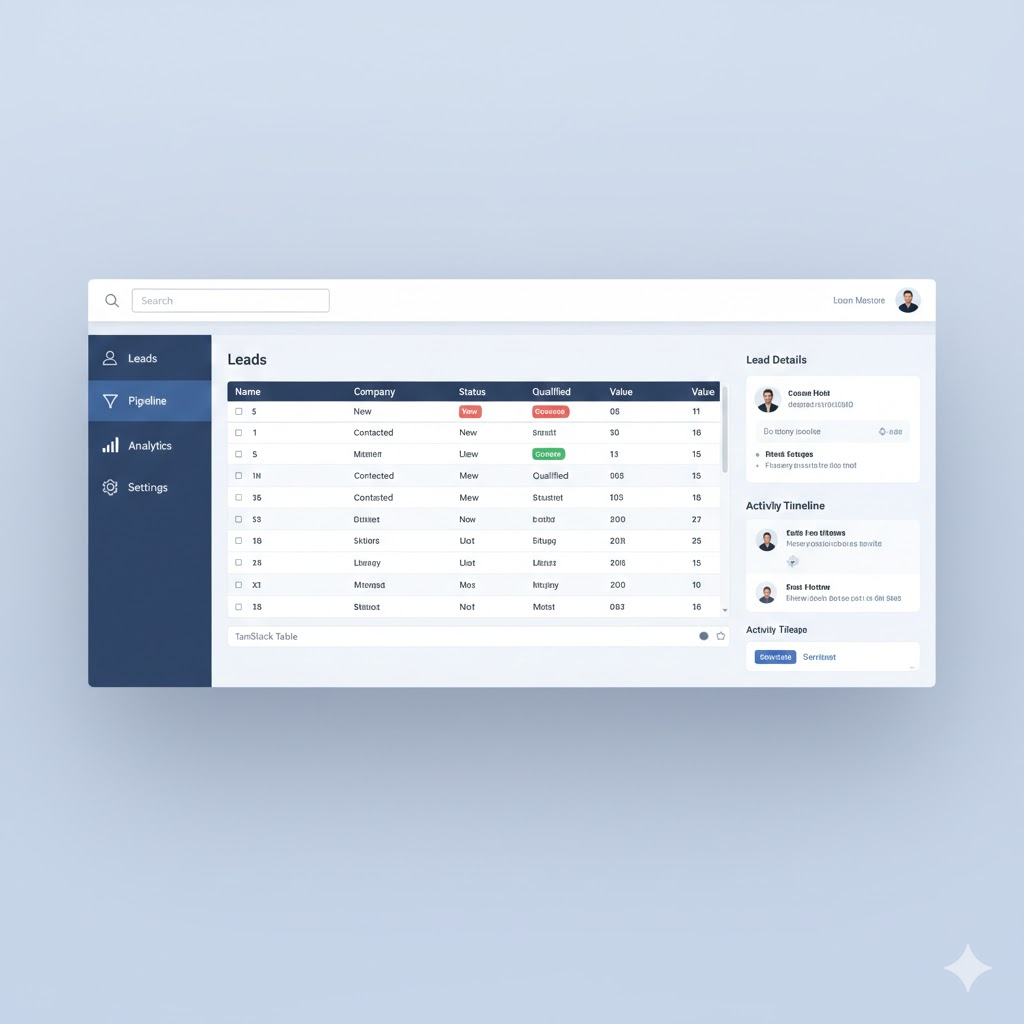
\includegraphics[width=\textwidth,height=0.82\textheight,keepaspectratio]{images/concept.jpg}
    \caption{Aperçu de notre solution CRM}
    \label{fig:notre-solution}
\end{figure}
\FloatBarrier

\section{Méthodologie de développement}

\subsection{Étude des méthodes existantes}
\label{sec:etude-methodes}
Plusieurs méthodologies de développement ont été étudiées pour choisir celle la plus adaptée à un projet agile et technique :

\subsubsection{Scrum}
Scrum est une méthode agile itérative et incrémentale, idéale pour les projets nécessitant une forte adaptabilité. Elle se caractérise par des sprints courts (2-4 semaines), des rituels réguliers (daily stand-up, sprint planning, review, retrospective) et une forte collaboration avec le client.

\begin{figure}[!htbp]
    \centering
    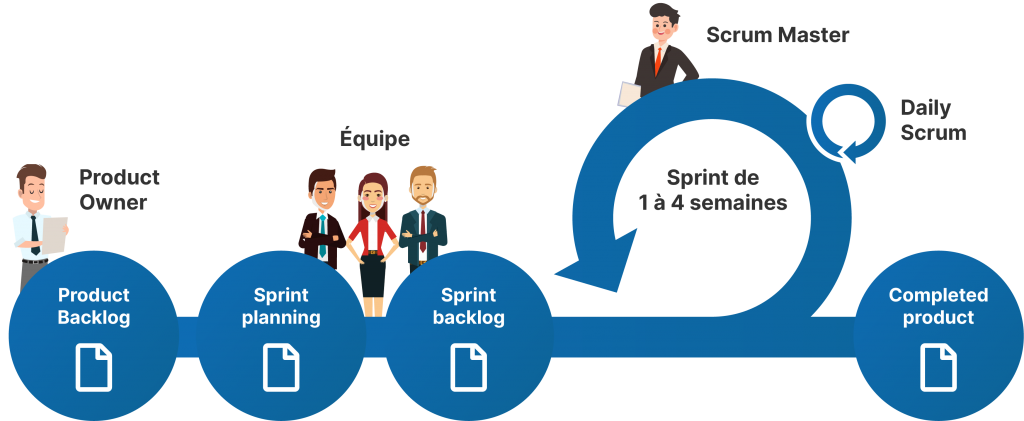
\includegraphics[width=\textwidth,height=0.82\textheight,keepaspectratio]{images/processus-scrum.png}
    \caption{Processus Scrum}
    \label{fig:scrum}
\end{figure}
\FloatBarrier

\subsubsection{Extreme Programming (XP)}
Extreme Programming (XP) met l'accent sur la qualité du code, les tests automatisés et l'intégration continue. Ses valeurs principales sont la simplicité, la communication, le feedback et le courage. XP est particulièrement adaptée aux projets nécessitant une grande flexibilité face aux changements de requirements.

\begin{figure}[!htbp]
    \centering
    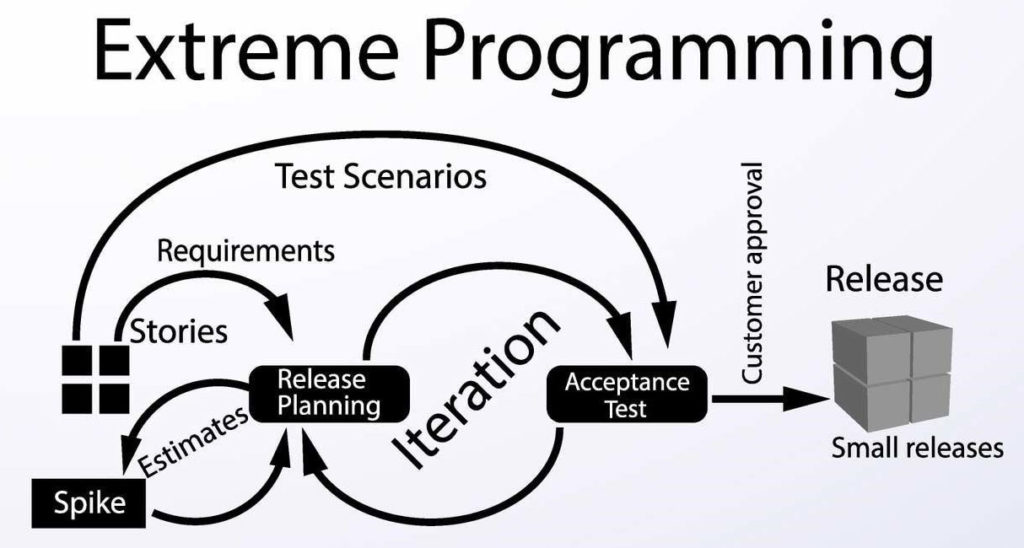
\includegraphics[width=\textwidth,height=0.82\textheight,keepaspectratio]{images/processus-xp.jpeg}
    \caption{Processus Extreme Programming (XP)}
    \label{fig:xp}
\end{figure}
\FloatBarrier

\subsubsection{Kanban}
Kanban permet une visualisation claire du flux de travail et une limitation des tâches en cours. Basée sur le système de production Toyota, cette méthode utilise un tableau avec des colonnes (To Do, In Progress, Done) pour visualiser l'avancement des tâches et identifier les goulots d'étranglement.

\begin{figure}[!htbp]
    \centering
    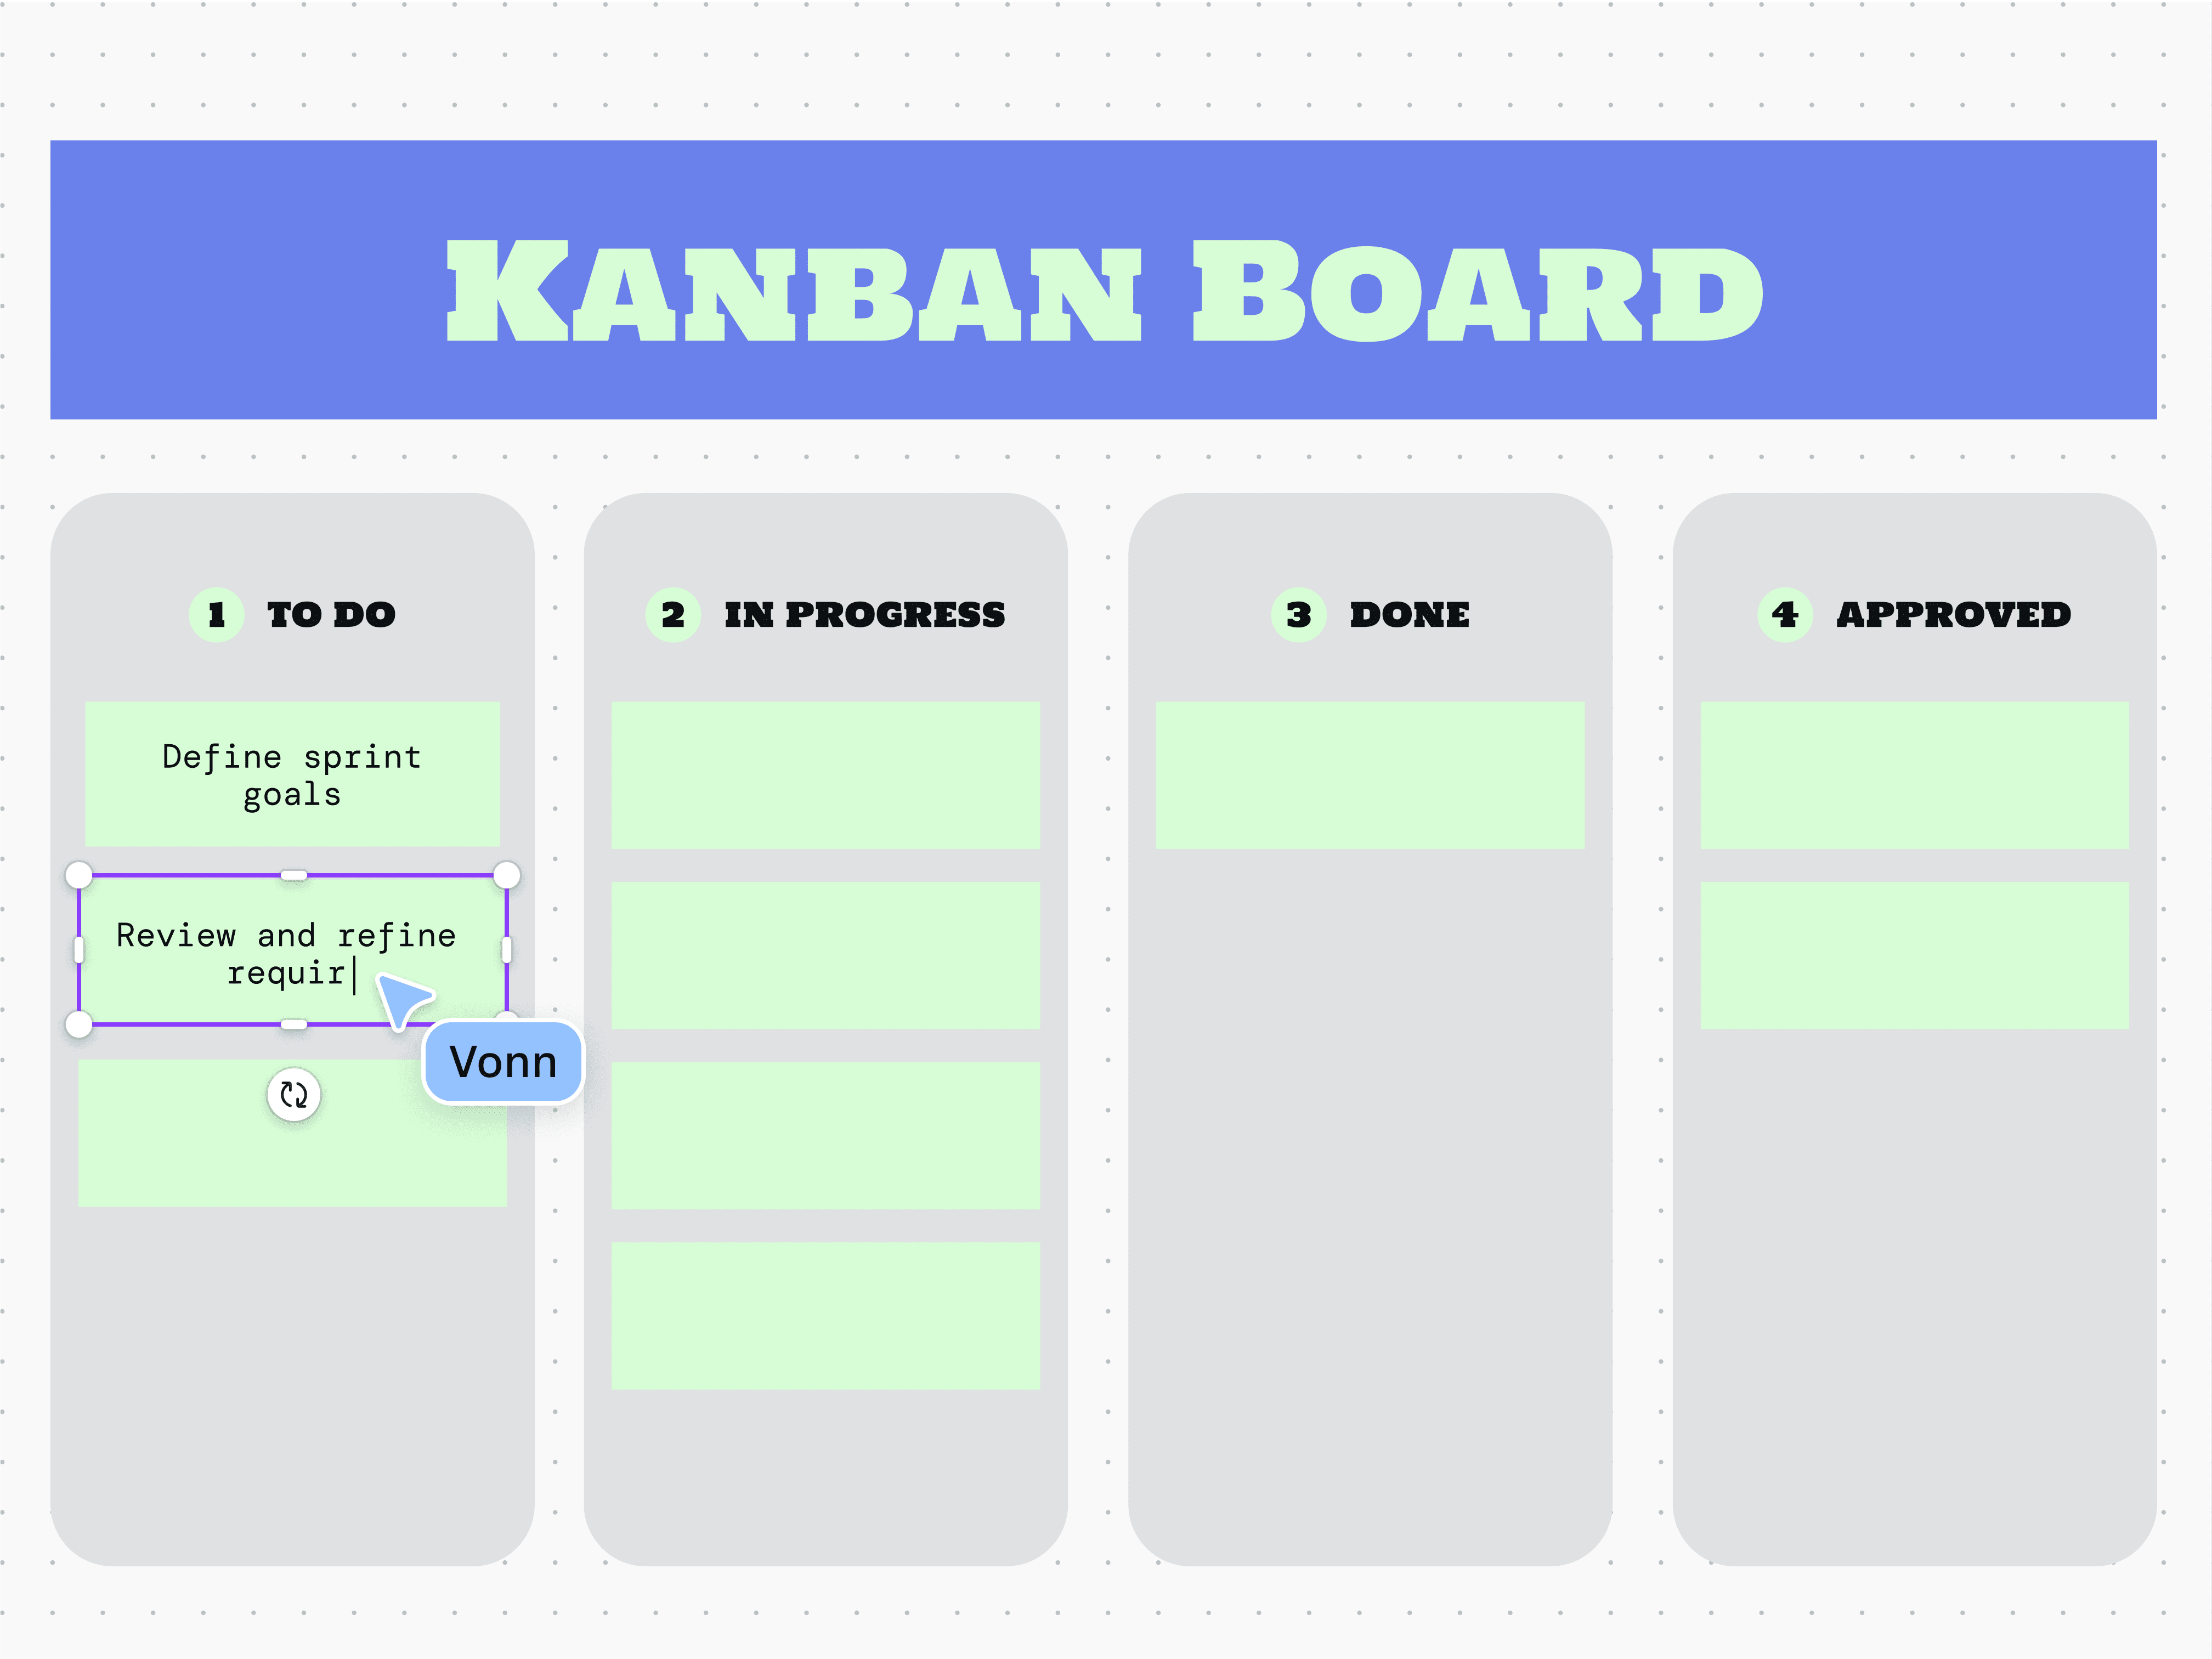
\includegraphics[width=\textwidth,height=0.82\textheight,keepaspectratio]{images/kanban.png}
    \caption{Processus Kanban}
    \label{fig:kanban}
\end{figure}
\FloatBarrier

\subsubsection{Waterfall (Cascade)}
La méthode Waterfall (ou en cascade) suit une approche séquentielle linéaire avec des phases bien définies : Conception, Implémentation, Test, Déploiement, Maintenance. Chaque phase doit être complétée avant de passer à la suivante, ce qui la rend prévisible mais peu flexible.

\begin{figure}[!htbp]
    \centering
    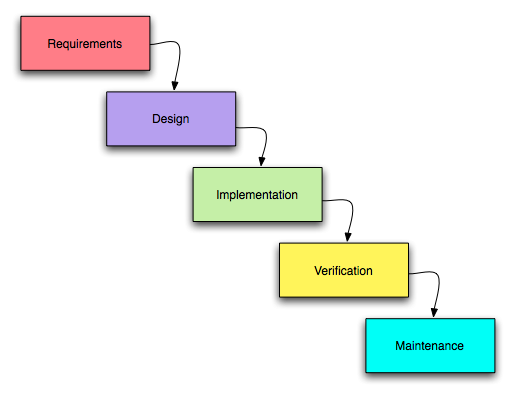
\includegraphics[width=\textwidth,height=0.82\textheight,keepaspectratio]{images/waterfall.png}
    \caption{Processus Waterfall (Cascade)}
    \label{fig:waterfall}
\end{figure}
\FloatBarrier

\subsubsection{Unified Process (UP)}
Unified Process est une méthodologie itérative et incrémentale qui combine des éléments des méthodes agiles et traditionnelles. Elle se décompose en quatre phases : Inception, Elaboration, Construction, Transition.

\begin{figure}[!htbp]
    \centering
    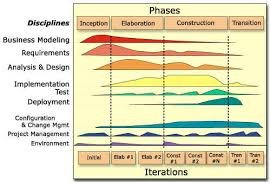
\includegraphics[width=\textwidth,height=0.82\textheight,keepaspectratio]{images/up.jpg}
    \caption{Processus Unified Process (UP)}
    \label{fig:up}
\end{figure}
\FloatBarrier

\subsubsection{Two-Track Unified Process (2TUP)}
2TUP est une variante d'UP qui sépare le développement en deux pistes parallèles : une piste fonctionnelle (métier) et une piste technique (architecture). Cette séparation permet une meilleure gestion des changements et une plus grande flexibilité.

\begin{figure}[!htbp]
    \centering
    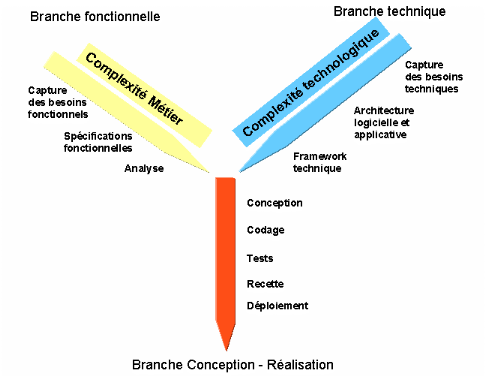
\includegraphics[width=\textwidth,height=0.82\textheight,keepaspectratio]{images/tup.png}
    \caption{Processus Two-Track Unified Process (2TUP)}
    \label{fig:2tup}
\end{figure}
\FloatBarrier

\subsection{Choix de la méthodologie}
Après analyse des différentes méthodes présentées dans la section \ref{sec:etude-methodes}, nous avons opté pour la méthodologie \textbf{2TUP} (Two-Track Unified Process) comme processus de développement principal pour notre projet CRM Micro-SaaS.

\subsubsection{Raisons du choix de 2TUP}
Le choix de 2TUP repose sur plusieurs raisons fondamentales qui correspondent parfaitement aux contraintes et aux objectifs de notre projet :

\begin{enumerate}
    \item \textbf{Séparation claire entre la branche fonctionnelle et la branche technique :}
    Notre projet CRM comporte deux dimensions très distinctes. D'un côté, une \textit{branche fonctionnelle} riche (gestion des leads, pipeline commercial, tickets de support, génération d'emails par IA, scoring prédictif) qui nécessite une analyse métier approfondie. De l'autre, une \textit{branche technique} complexe (architecture micro-services, intégration d'API externes comme Google Gemini et FastAPI, conteneurisation Docker/Kubernetes, ORM Prisma). 2TUP permet de mener ces deux pistes en parallèle avant de les fusionner lors de la phase de conception, ce qui est idéal pour notre contexte.

    \item \textbf{Approche itérative et incrémentale adaptée aux sprints du projet :}
    2TUP suit un cycle de vie itératif et incrémental, ce qui s'aligne directement avec notre planification en \textbf{4 sprints} successifs (Conception \& BDD, API \& Frontend, UI \& Tests, Documentation \& Soutenance). Chaque sprint produit un livrable fonctionnel et testable, permettant une validation progressive du système.

    \item \textbf{Compatibilité native avec le formalisme UML :}
    2TUP, en tant que variante du Unified Process, s'appuie nativement sur le langage de modélisation \textbf{UML} pour la spécification, la conception et la documentation. Cela garantit une cohérence totale entre notre méthodologie et nos livrables de modélisation (diagrammes de cas d'utilisation, de séquence, de classes et de déploiement).

    \item \textbf{Gestion maîtrisée des risques techniques :}
    L'intégration de services d'intelligence artificielle (API Gemini, micro-service de scoring) introduit des risques techniques importants (latence réseau, indisponibilité des API, qualité des prédictions). La branche technique de 2TUP permet d'identifier et de traiter ces risques architecturaux dès les premières phases, notamment à travers les mécanismes de \textit{fallback} (Graceful Degradation) que nous avons mis en place.

    \item \textbf{Flexibilité face aux changements de spécifications :}
    Dans le cadre d'un projet de fin d'études réalisé au sein d'une entreprise (VisioAd), les exigences peuvent évoluer en cours de développement. Contrairement à la méthode Waterfall qui fige les spécifications, 2TUP offre une souplesse d'adaptation grâce à ses itérations successives, tout en conservant une rigueur de documentation supérieure aux méthodes purement agiles.
\end{enumerate}

\begin{figure}[!htbp]
    \centering
    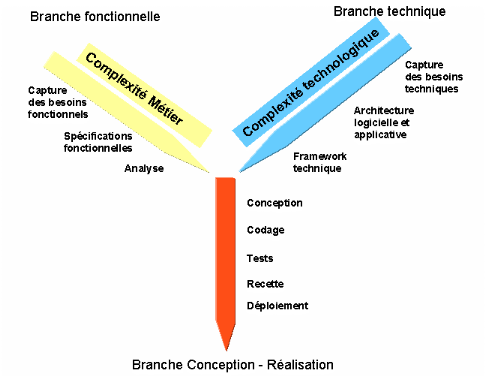
\includegraphics[width=\textwidth,height=0.82\textheight,keepaspectratio]{images/tup.png}
    \caption{Processus 2TUP adopté pour le projet CRM}
    \label{fig:methode-2tup-choix}
\end{figure}
\FloatBarrier

\subsection{Choix des formalismes adéquats}
Pour la modélisation et la documentation de notre système, nous avons adopté le langage \textbf{UML} (Unified Modeling Language) comme formalisme de référence. Ce choix se justifie par les raisons suivantes :

\begin{itemize}
    \item \textbf{Standard universel :} UML est le langage de modélisation le plus répandu dans l'industrie du génie logiciel, ce qui facilite la communication entre les parties prenantes du projet.
    \item \textbf{Cohérence avec 2TUP :} Le processus 2TUP repose intrinsèquement sur les diagrammes UML pour formaliser les résultats de chaque phase (branche fonctionnelle et branche technique).
    \item \textbf{Couverture complète :} UML offre une palette de diagrammes couvrant tous les aspects de notre système :
    \begin{itemize}
        \item \textit{Diagrammes de cas d'utilisation} pour capturer les besoins fonctionnels par acteur.
        \item \textit{Diagrammes de séquence système} pour modéliser les interactions temporelles entre les composants (Frontend, Backend, API IA).
        \item \textit{Diagramme de classes} pour structurer le modèle de données et les relations entre entités.
        \item \textit{Diagramme de déploiement} pour représenter l'architecture physique micro-services (Next.js, NestJS, FastAPI, MySQL, Docker).
    \end{itemize}
    \item \textbf{Outil de documentation pérenne :} Les diagrammes UML constituent une documentation technique durable, facilitant la maintenance et l'évolution future du CRM.
\end{itemize}

\section{Planification}
Au départ, on a dessiné un graphique pour voir comment se passe le travail. Chaque étape importante apparaît dedans, avec des dates étalées de février à juillet. Grâce à ce repère visuel, il est plus simple de mesurer où en est le chantier. Quelque chose change ? On réorganise sans tarder selon les besoins du moment.

\begin{figure}[!htbp]
    \centering
    \resizebox{\textwidth}{!}{
    \renewcommand{\arraystretch}{1.5} % Espace entre les lignes
    \begin{tabular}{|p{7.5cm}|*{16}{c|}}
    \hline
    \rowcolor{gray!70}
    \textbf{\textcolor{white}{Tâches / User Stories}} & 
    \multicolumn{4}{c|}{\cellcolor{blue!70}\textbf{\textcolor{white}{Incrément 1 : Conception \& BDD}}} & 
    \multicolumn{4}{c|}{\cellcolor{red!70}\textbf{\textcolor{white}{Incrément 2 : API \& Frontend}}} & 
    \multicolumn{4}{c|}{\cellcolor{orange!70}\textbf{\textcolor{white}{Incrément 3 : UI \& Tests}}} & 
    \multicolumn{4}{c|}{\cellcolor{green!70}\textbf{\textcolor{white}{Incrément 4 : Doc \& Soutenance}}} \\
    \hline
    \rowcolor{gray!20}
    \textbf{Période $\rightarrow$ Sem.} & 
    \textbf{S1} & \textbf{S2} & \textbf{S3} & \textbf{S4} & 
    \textbf{S5} & \textbf{S6} & \textbf{S7} & \textbf{S8} & 
    \textbf{S9} & \textbf{S10} & \textbf{S11} & \textbf{S12} & 
    \textbf{S13} & \textbf{S14} & \textbf{S15} & \textbf{S16} \\
    \hline
    
    % SPRINT 1
    \multicolumn{17}{|l|}{\cellcolor{gray!10}\textbf{SPRINT 1 TASKS}} \\
    \hline
    US-01 : Analyse des besoins et conception & \cellcolor{blue!50} & \cellcolor{blue!50} & & & & & & & & & & & & & & \\
    \hline
    US-02 : Développement de la base de données & & & \cellcolor{blue!50} & \cellcolor{blue!50} & & & & & & & & & & & & \\
    \hline
    
    % SPRINT 2
    \multicolumn{17}{|l|}{\cellcolor{gray!10}\textbf{SPRINT 2 TASKS}} \\
    \hline
    US-03 : Développement de l'API backend & & & & & \cellcolor{red!50} & \cellcolor{red!50} & & & & & & & & & & \\
    \hline
    US-04 : Développement du frontend (Interface) & & & & & & & \cellcolor{red!50} & \cellcolor{red!50} & & & & & & & & \\
    \hline
    
    % SPRINT 3
    \multicolumn{17}{|l|}{\cellcolor{gray!10}\textbf{SPRINT 3 TASKS}} \\
    \hline
    US-05 : Développement frontend (Virtualisation) & & & & & & & & & \cellcolor{orange!50} & \cellcolor{orange!50} & & & & & & \\
    \hline
    US-06 : Tests et optimisation des performances & & & & & & & & & & & \cellcolor{orange!50} & \cellcolor{orange!50} & & & & \\
    \hline
    
    % SPRINT 4
    \multicolumn{17}{|l|}{\cellcolor{gray!10}\textbf{SPRINT 4 TASKS}} \\
    \hline
    US-07 : Documentation et préparation démo & & & & & & & & & & & & & \cellcolor{green!50} & \cellcolor{green!50} & & \\
    \hline
    US-08 : Soutenance et livraison finale & & & & & & & & & & & & & & & \cellcolor{green!50} & \cellcolor{green!50} \\
    \hline
    
    % Timeline du bas
    \rowcolor{gray!20}
    \textbf{Mois} & \multicolumn{4}{c|}{\textbf{Février - Mars 2026}} & \multicolumn{4}{c|}{\textbf{Avril - Mai 2026}} & \multicolumn{4}{c|}{\textbf{Juin 2026}} & \multicolumn{4}{c|}{\textbf{Juillet 2026 (Soutenance)}} \\
    \hline
    \end{tabular}
    }
    \caption{Diagramme de Gantt du projet CRM (Février à Juillet - 4 Incréments)}
    \label{fig:gantt}
\end{figure}
\FloatBarrier

Les principales phases du projet sont :
\begin{itemize}
    \item \textbf{Semaines 1-2} : Analyse des besoins et conception initiale
    \item \textbf{Semaines 3-6} : Développement du backend (API, base de données)
    \item \textbf{Semaines 7-10} : Développement du frontend (interface, virtualisation)
    \item \textbf{Semaines 11-12} : Tests et optimisation des performances
    \item \textbf{Semaines 13-14} : Documentation et préparation de la démonstration
    \item \textbf{Semaines 15-16} : Revue finale et corrections
\end{itemize}

\section{Conclusion}
Dans ce chapitre, nous avons posé le cadre général du projet en commençant par la présentation de l'organisme d'accueil VisioAd et de ses activités. Ensuite, une étude comparative approfondie des CRM existants sur le marché — Salesforce, HubSpot et Zoho — a permis d'identifier leurs forces et leurs limites, et de positionner notre solution comme une alternative adaptée aux petites équipes B2B. Après un examen des méthodologies de développement existantes, notre choix s'est porté sur le processus \textbf{2TUP} (Two-Track Unified Process), dont la séparation en branche fonctionnelle et branche technique correspond idéalement à la double nature de notre projet. Le formalisme \textbf{UML} a été retenu pour la modélisation, en parfaite cohérence avec 2TUP. Enfin, la planification a été structurée en quatre sprints répartis sur seize semaines, de février à juillet 2026, permettant une livraison progressive et maîtrisée du système. Le chapitre suivant se consacrera à l'analyse et à la spécification détaillée des besoins fonctionnels et non fonctionnels.

\clearpage

% Chapitre 2 (page 9)
\chapter{Analyse et spécification des besoins}
\label{chap:analyse_besoins}
\section*{Introduction}
\addcontentsline{toc}{section}{Introduction}
La spécification des besoins constitue une étape essentielle dans le développement d’un projet.
Elle permet de passer d’une vision abstraite du sujet à une définition concrète du produit,
en comprenant clairement le travail qui reste à faire. Cette étape est aujourd’hui d’autant plus
critique car elle doit piloter la rencontre entre la gestion des big data, le pilotage commercial
traditionnel et l’adjonction de solutions d’IA prédictives ou génératives dans le cadre de ce
projet de CRM smart avec moteur de lead scoring par IA.

Dans ce chapitre, nous commencerons par identifier les différents acteurs impliqués et leurs
rôles respectifs, puis nous déterminerons les exigences fonctionnelles et non fonctionnelles que
notre système doit répondre. Enfin, nous effectuerons une modélisation UML complète, struc-
turée par acteur et par cas d’utilisation précis, pour aboutir à une application qui réponde par-
faitement aux besoins des utilisateurs.

\section{Identification des acteurs}

Selon les formalismes UML, un acteur définit un rôle externe qui interagit avec le système
pour en obtenir une valeur ajoutée. Le cœur de notre CRM intelligent réside dans une synergie
entre des acteurs humains, avec des rôles hiérarchisés, et des services d’intelligence artificielle
qui améliorent l’expérience utilisateur.

\subsection*{Acteurs principaux}

\begin{itemize}
    \item \textbf{Sales Representative (Commercial)} : C’est l’acteur opérationnel au cœur du système.
    Sa mission consiste à convertir des opportunités commerciales potentielles en ventes
    réelles. Il se connecte à la plateforme pour voir et gérer ses leads assignés, piloter ses
    contacts et deals, planifier ses activités quotidiennes (appels, tâches, réunions) et utiliser
    les outils d’intelligence artificielle afin de personnaliser sa communication. Pour lui, le
    CRM devient un assistant proactif qui priorise son travail grâce au scoring prédictif et
    automatise ses rédactions grâce à l’IA Gemini.
    
    \item \textbf{Sales Manager / Administrateur} : Il intervient au plan stratégique et technique. Il
    est en charge de l’intégrité de la plateforme, de la gestion des comptes utilisateurs et
    de l’analyse des performances de l’ensemble de l’équipe commerciale. Il joue un rôle
    clé dans les phases de migration de données, orchestrant les modules d’importation de
    masse à partir de fichiers CSV. Il a également accès à toutes les analytics et les tableaux
    de bord, lui permettant d’adapter la stratégie commerciale en fonction des indicateurs
    donnés par le système.
\end{itemize}

\subsection*{Acteurs secondaires (Systèmes)}

Notre application repose sur des services externes dont les contrats d’interface donnent la possibilité de traiter et d’accéder aux données du système. Les systèmes utilisés sont les sui-
vants :

\begin{itemize}
    \item \textbf{Système Gemini API — Google} : Google Gemini (modèle gemini-1.5-flash) fonctionne comme un service de traitement du langage naturel (NLP) pour la génération automa-
    tique de contenu personnalisé. Ce service permet de rédiger des brouillons d’emails commerciaux adaptés en analysant les données contextuelles d’un prospect (notes, histo-
    rique d’emails, score IA, informations sur l’entreprise). De plus, il propulse un assistant conversationnel (Chatbot) intelligent qui utilise l’approche RAG (Retrieval-Augmented Generation) pour répondre en temps réel aux questions de l’utilisateur sur les données CRM.
    
    \item \textbf{Lead Scoring AI Agent (Micro-service FastAPI)} : C’est un micro-service Python conçu pour l’analyse prédictive, développé avec le framework FastAPI. Il offre l’endpoint \texttt{POST /predict-score} qui reçoit les caractéristiques comportementales et contex-
    tuelles d’un lead. Il renvoie un score de conversion sur 100 et une catégorie qualitative (Hot, Warm, ou Cold) produite par un modèle RandomForestClassifier entraîné.
    
    \item \textbf{Système de gestion de base de données MySQL} : C’est le système de gestion de base de données relationnelle qui garantit la persistance de toutes les données de l’application. Ce système est géré grâce à l’ORM Prisma, qui assure la protection des requêtes et l’uniformité du schéma de données.
\end{itemize}

\section{Spécification des besoins}

Cette section vise à rassembler, examiner et établir les besoins fondamentaux et les caracté-
ristiques du projet. Elle met l’accent sur les besoins fonctionnels et non fonctionnels indispen-
sables pour offrir des services simples à utiliser et à entretenir.

\subsection{Les besoins fonctionnels}

Les exigences fonctionnelles définissent les attentes de chaque intervenant concernant l’ap-
plication à concevoir. Dans le contexte de notre projet, nous avons repéré les exigences fonc-
tionnelles qui suivent :

\begin{itemize}
    \item \textbf{Connexion} : L’utilisateur se connecte à l’application en entrant ses informations d’iden-
    tification (adresse électronique et mot de passe). Le système produit un jeton JWT si-
    gné qui permet l’accès aux ressources sécurisées en fonction du rôle de l’utilisateur, soit ADMIN ou REP.
    
    \item \textbf{Gestion des Prospects} : L’utilisateur a la possibilité de créer, visualiser, modifier et éliminer des prospects. Chaque piste est liée à une étape de cycle de vie (NOUVEAU, CONTACTÉ, QUALIFIÉ, PERDU), une estimation de la valeur de l’affaire, des rensei-
    gnements sur la société et un score IA qui est automatiquement calculé par le micro-
    service prédictif.
    
    \item \textbf{Vérification du Score IA d’un Lead} : L’utilisateur est en mesure de déclencher le calcul de la probabilité de conversion d’un lead. Le système sollicite le micro-service FastAPI par l’intermédiaire de \texttt{POST /predict-score} et présente la réponse sous la forme d’un score quantitatif (0-100) complété par une évaluation qualitative de la température (Hot/Warm/Cold) et une série d’arguments explicatifs.
    
    \item \textbf{Produire un courrier électronique grâce à l’IA (Gemini)} : L’utilisateur a la possibilité de solliciter la création d’un projet de courrier électronique sur mesure pour un prospect. Le système évalue le contexte du prospect et sollicite l’API Google Gemini afin de générer un contenu sur mesure. Si l’API n’est pas disponible, un système de règles fixes est utilisé en remplacement (on parle alors de « Graceful Degradation »).
    
    \item \textbf{Assistant conversationnel intelligent (RAG avec Gemini)} : L’utilisateur dispose d’un assistant virtuel (chatbot) pour interroger les données du CRM en langage naturel. Le backend NestJS extrait dynamiquement le contexte lié aux prospects, deals et statis-
    tiques globales depuis MySQL pour alimenter le modèle Gemini, permettant des ré-
    ponses ultra-ciblées sur les données réelles et empêchant les réponses aléatoires.
    
    \item \textbf{Administration des Contacts} : L’utilisateur a la possibilité de créer, visualiser, changer et effacer des contacts clients. Chaque contact est associé à une entreprise et peut être lié à de multiples pistes, activités et demandes d’assistance.
    
    \item \textbf{Administration des Entreprises (Companies)} : L’utilisateur a la possibilité de gérer l’inventaire des entreprises clients ou en perspective, comprenant leurs informations dé-
    taillées (domaine d’activité, dimension, site internet, pays).
    
    \item \textbf{Administration du Pipeline Commercial (Transactions)} : L’utilisateur a la possibi-
    lité d’établir et de suivre des prospects commerciaux via un pipeline de vente visuel en format Kanban. Chaque transaction est liée à une somme d’argent, une date de fin approximative et un état (PENDING, ACTIVE, WON, LOST).
    
    \item \textbf{Administration des Activités} : L’utilisateur a la possibilité de programmer et d’or-
    ganiser ses interactions professionnelles : appel téléphonique, envoi d’email, réunion ou tâche. Chaque action est associée à un prospect ou un contact et peut être indiquée comme terminée.
    
    \item \textbf{Administration des Billets de Support} : L’usager a la possibilité de générer des de-
    mandes d’assistance pour identifier et suivre les problèmes ou requêtes. Les tickets passent par une séquence de statuts (NEW, OPEN, PENDING, RESOLVED, CLOSED) et sont classés selon un niveau de priorité (LOW, MEDIUM, HIGH, CRITICAL).
    
    \item \textbf{Importation massive de données (CSV)} : Il est possible pour l’administrateur d’im-
    porter plus de 1 000 enregistrements (contacts, leads ou entreprises) à partir d’un fichier CSV. Le système valide chaque ligne, détecte les doublons par une clé composite (Email + UserId) et génère un rapport d’importation synthétique.
    
    \item \textbf{Accéder aux Tableaux de Bord et aux Analyses} : L’administrateur peut consulter des tableaux de bord dynamiques qui récapitulent les indicateurs clés de performance (KPIs) de l’équipe commerciale : le taux de transformation, la distribution des prospects selon leur statut, la valeur globale du pipeline et les résultats par représentant commercial.
    
    \item \textbf{Gestion des Comptes Utilisateurs} : L’administrateur a la possibilité de créer, changer, activer ou désactiver les comptes des membres de l’équipe, en leur attribuant le rôle adéquat.
    
    \item \textbf{Obtenir des Notifications} : L’utilisateur est averti en direct par le système lors d’évé-
    nements essentiels : l’arrivée d’un nouveau prospect prometteur, l’approche imminente d’une tâche, ou la mise à jour de la situation d’un ticket.
\end{itemize}

\subsection{Les besoins non fonctionnels}

Les exigences non fonctionnelles se referent aux besoins opérationnels qui définissent la
qualité du système. Pour notre application, nous avons défini et intégré les exigences non
fonctionnelles suivantes :

\subsubsection{A. Sécurité et Confidentialité}

La sécurité est une priorité absolue, particulièrement pour un CRM manipulant des données clients sensibles.

\begin{itemize}
    \item \textbf{Où et comment c’est intégré :}
    \begin{itemize}
        \item \textbf{Authentification} : Intégrée au niveau du backend (NestJS) via des jetons JWT sto-
        ckés et gérés par les Guards (ex. JwtAuthGuard) pour sécuriser les routes.
        \item \textbf{Autorisation (RBAC)} : Déployée à l’aide des décorateurs personnalisés (ex. décorateur \texttt{@Roles('ADMIN')} dans les contrôleurs NestJS) pour bloquer l’accès non autorisé aux routes critiques (comme l’import CSV ou la gestion de tous les comptes).
        \item \textbf{Isolation des données} : Implémentée dans les services (Services) via Prisma, où les requêtes SQL (ex. userId: req.user.id) filtrent systématiquement les entités (leads, contacts, deals) selon l’utilisateur connecté pour empêcher les accès croisés.
        \item \textbf{Chiffrement} : Utilisé lors de la création et de la mise à jour des mots de passe grâce à l’algorithme Bcrypt dans le module utilisateur.
    \end{itemize}
\end{itemize}

\subsubsection{B. Performance et Réactivité}

L’application doit répondre instantanément pour garantir la productivité des commerciaux.

\begin{itemize}
    \item \textbf{Où et comment c’est intégré :}
    \begin{itemize}
        \item \textbf{Rendu Frontend} : Utilisé de manière globale via le framework Next.js (App Rou-
        ter) qui pré-génère les pages côté serveur (SSR) et garantit des temps de chargement réduits.
        \item \textbf{Optimisation des bases de données} : Intégrée dans le schéma Prisma en définissant des index sur les clés étrangères pour accélérer les jointures. Par exemple : \texttt{@index([userId])} et \texttt{@index([companyId])}, ce qui améliore les performances lors de l’affichage des tableaux de bord analytiques complexes.
        \item \textbf{Mises à jour en temps réel (Triggers)} : Implémentées dans le frontend via les hooks useEffect qui "écoutent" les modifications d'état (ajout de notes, tâches complétées) pour re-fetcher dynamiquement les données statistiques sans rafraîchir la page.
    \end{itemize}
\end{itemize}

\subsubsection{C. Disponibilité, Résilience et Tolérance aux pannes}

Le CRM doit rester opérationnel même en cas de défaillance partielle des services tiers.

\begin{itemize}
    \item \textbf{Où et comment c’est intégré :}
    \begin{itemize}
        \item \textbf{Mécanisme de Fallback (Graceful Degradation)} : Intégré dans le service \texttt{ai-email.service} — si l’API Google Gemini échoue, un email générique est généré à partir de modèles locaux. De même, si le micro-service FastAPI ne répond pas, un algorithme de secours fondé sur des règles calcule un score de repli.
        \item \textbf{Gestion des erreurs globales} : Implémentée via des Exception Filters dans NestJS et des Toast Notifications (avec react-hot-toast) dans Next.js pour avertir l’utilisateur d’un problème sans faire crasher l’application logicielle.
    \end{itemize}
\end{itemize}

\subsubsection{D. Évolutivité et Scalabilité}

L’architecture doit pouvoir supporter une augmentation du nombre d’utilisateurs et de la quantité de données gérées.

\begin{itemize}
    \item \textbf{Où et comment c’est intégré :}
    \begin{itemize}
        \item \textbf{Architecture Micro-services} : Le découpage du projet en trois entités distinctes (Frontend Next.js, Backend NestJS, Agent IA FastAPI) permet d’allouer plus de ressources de manière granulaire, uniquement au service qui en a besoin (ex. scaler FastAPI lors d’un pic d’analyses prédictives).
        \item \textbf{Conteneurisation} : Utilisation de Docker (via les fichiers Dockerfile et docker-compose) pour garantir que chaque composant est isolé et peut être déployé ou mis à l’échelle sur le cloud sans conflit de dépendances.
    \end{itemize}
\end{itemize}

\subsubsection{E. Maintenabilité et Qualité du Code}

Le code doit être facilement compréhensible et modifiable par de nouveaux développeurs rejoignant le projet.

\begin{itemize}
    \item \textbf{Où et comment c’est intégré :}
    \begin{itemize}
        \item \textbf{Typage fort} : Application stricte de TypeScript partagée entre le frontend et le backend pour prévenir les anomalies au moment de la compilation.
        \item \textbf{Architecture Modulaire} : Implémentée dans NestJS à travers le concept de Modules (ex. LeadsModule, AnalyticsModule), en séparant très clairement les responsabilités MVC (Controllers, Services, DTOs).
        \item \textbf{ORM Centralisé} : L’utilisation du fichier schema.prisma qui agit comme source unique de vérité pour le modèle de données, facilitant la gestion des migrations lors de modifications de la base.
    \end{itemize}
\end{itemize}

\subsubsection{F. Ergonomie et Utilisabilité (UX/UI)}

Le système doit être intuitif, esthétique et facile à prendre en main pour réduire le temps de formation des utilisateurs commerciaux.

\begin{itemize}
    \item \textbf{Où et comment c’est intégré :}
    \begin{itemize}
        \item \textbf{Composants Visuels} : Construits dans l’interface utilisateur en exploitant le frame-
        work Tailwind CSS et les icônes de Lucide React pour une consistance visuelle moderne et compréhensible.
        \item \textbf{Comportement Réactif (Responsive)} : Le design des interfaces (Tableaux, Kan-
        bans, Modules de détails) est nativement conçu pour s’adapter et rester fonctionnel sur de multiples résolutions d’écran.
        \item \textbf{Feedback Visuel dynamique} : Application d’animations fluides lors d’actions clés (Drag \& Drop dans le Pipeline, micro-animations sur les graphiques analytiques) et de spinners de chargement lors d’appels asynchrones, rendant la plateforme "vi-
        vante".
    \end{itemize}
\end{itemize}

\subsubsection{G. Interopérabilité}

Le système doit être capable de communiquer de manière fluide et normée avec ses multiples services internes ou externes.

\begin{itemize}
    \item \textbf{Où et comment c’est intégré :}
    \begin{itemize}
        \item \textbf{Architecture API RESTful} : Le backend NestJS expose des points d’accès standards (endpoints) permettant au frontend de consommer les données de façon dé-
        couplée, facilitant la création éventuelle d’une future application mobile.
        \item \textbf{Protocoles Standardisés} : L’échange de données entre le backend principal et le micro-service d’Intelligence Artificielle (FastAPI) ainsi que les API externes (Google Gemini) se fait exclusivement en format JSON via HTTP, assurant une totale inter-
        opérabilité indépendamment des langages de programmation.
    \end{itemize}
\end{itemize}

\section{Diagrammes de cas d’utilisation}

Un diagramme de cas d’utilisation représente les fonctionnalités du système du point de vue de l’utilisateur et fournit une vision générale du comportement fonctionnel de l’application. La conceptualisation de ces diagrammes est une étape primordiale pour produire un logiciel conforme aux attentes des parties prenantes.

\subsection{Structuration en packages}

La structuration d’un modèle statique repose sur deux principes fondamentaux : la cohé-
rence et l’indépendance. Pour simplifier notre modèle, nous avons organisé les cas d’utilisation en les regroupant dans des ensembles fonctionnels cohérents, appelés packages, illustrés dans la figure 2.1.

\begin{figure}[H]
    \centering
     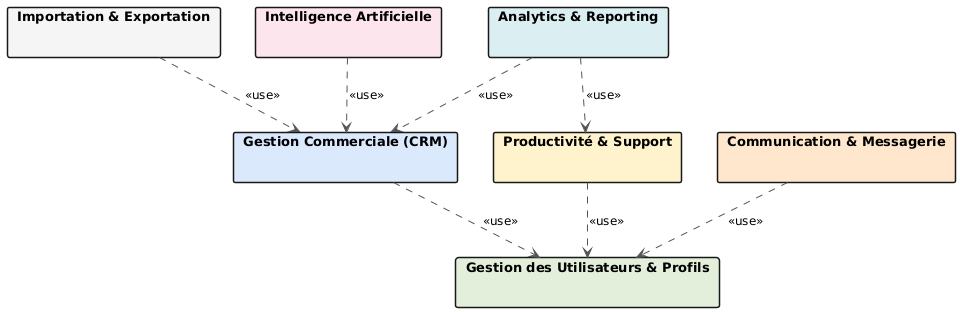
\includegraphics[width=0.85\textwidth]{images/packages_fonctionnels.png}
    \caption{Structuration en packages fonctionnels du système CRM}
    \label{fig:packages}
\end{figure}

\subsection{Diagramme de cas d’utilisation du côté « Sales Representative »}

Le diagramme de cas d’utilisation du côté « Sales Representative » est présenté ci-dessous dans la figure 2.2. Ce participant dispose d’un accès à l’ensemble des fonctionnalités du CRM indispensables pour mener à bien ses activités commerciales. Il communique directement avec deux systèmes externes : l’API Gemini pour la création d’emails, et le micro-service de notation IA pour juger ses prospects.

\begin{figure}[H]
    \centering
     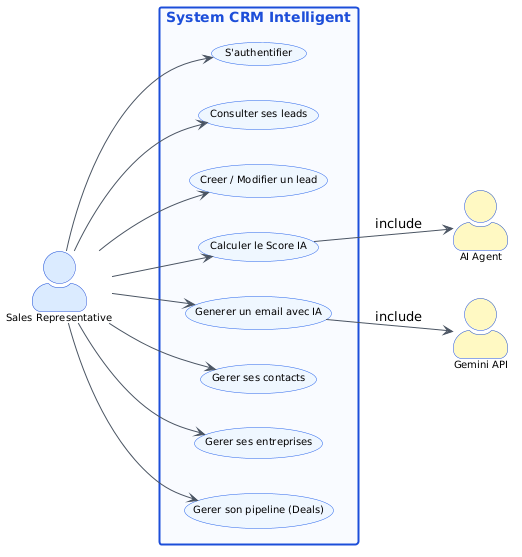
\includegraphics[width=0.9\textwidth]{images/uc_sales_rep.png}
    \caption{Diagramme de cas d’utilisation du côté « Sales Representative »}
    \label{fig:uc_sales_rep}
\end{figure}

\subsection{Diagramme de cas d’utilisation du côté « Administrateur »}

La figure 2.3 illustre les scénarios d’utilisation pour l’acteur « Administrateur / Sales Mana-
ger ». Outre les fonctionnalités opérationnelles disponibles pour le Représentant Commercial, l’administrateur a des privilèges uniques qui lui permettent de contrôler intégralement la plate-
forme : gestion des comptes, importation en grande quantité de données et accès à des analyses sophistiquées.

\begin{figure}[H]
    \centering
    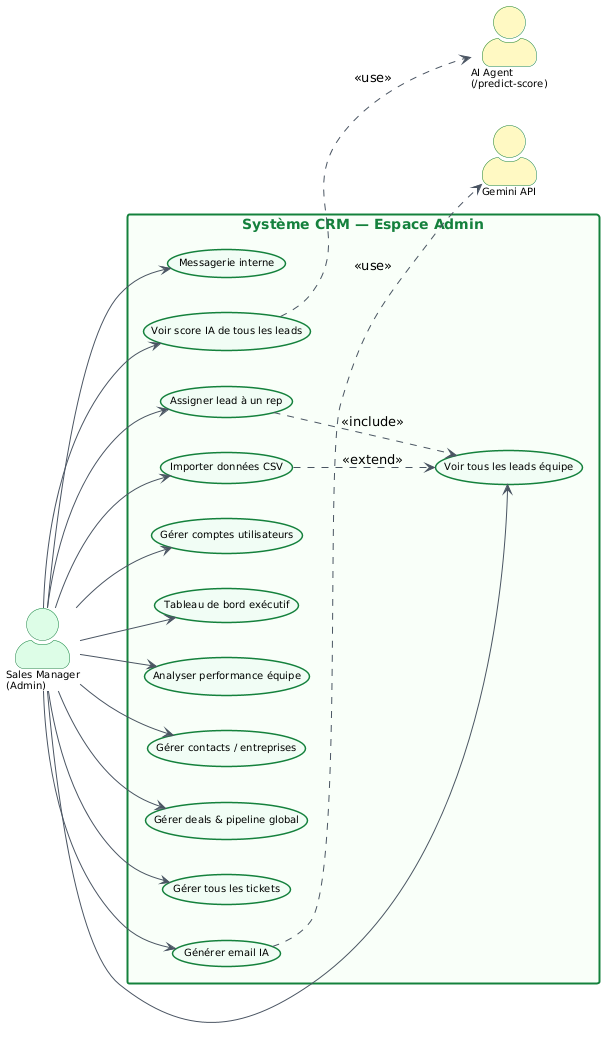
\includegraphics[width=0.9\textwidth]{images/uc_admin.png}
    \caption{Diagramme de cas d’utilisation du côté « Administrateur »}
    \label{fig:uc_admin}
\end{figure}

\subsection{Diagramme de cas d’utilisation relatif au cas d’utilisation « Gérer les Leads »}

Le diagramme de la figure 2.4, relatif au cas d’utilisation « Gérer les Leads », permet de visualiser de manière claire et concise les sous-cas d’utilisation associés. La gestion des leads englobe un cycle de vie complet allant de la création à la clôture, enrichi par les fonctionnalités d’intelligence artificielle. L’utilisateur peut créer un lead, mettre à jour son statut, consulter son score prédictif et générer un email personnalisé.

\begin{figure}[H]
    \centering
     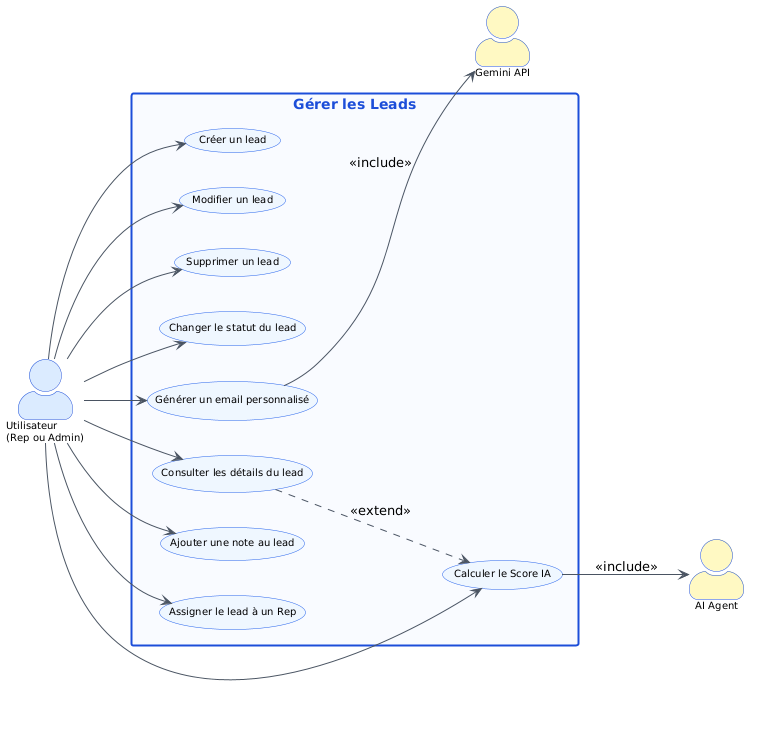
\includegraphics[width=0.8\textwidth]{images/uc_gerer_leads.png}
    \caption{Diagramme de cas d’utilisation relatif à « Gérer les Leads »}
    \label{fig:uc_gerer_leads}
\end{figure}

\subsection{Diagramme de cas d’utilisation relatif au cas d’utilisation « Importer des Données »}

Le diagramme de cas d’utilisation concernant l’« Importation de Données » est illustré à la figure 2.5. Ce cas d’utilisation, réservé à l’administrateur, détaille les étapes du processus d’importation de masse à partir d’un fichier CSV, incluant la validation de la structure du fichier, la détection de doublons et la génération d’un rapport final.

\begin{figure}[H]
    \centering
    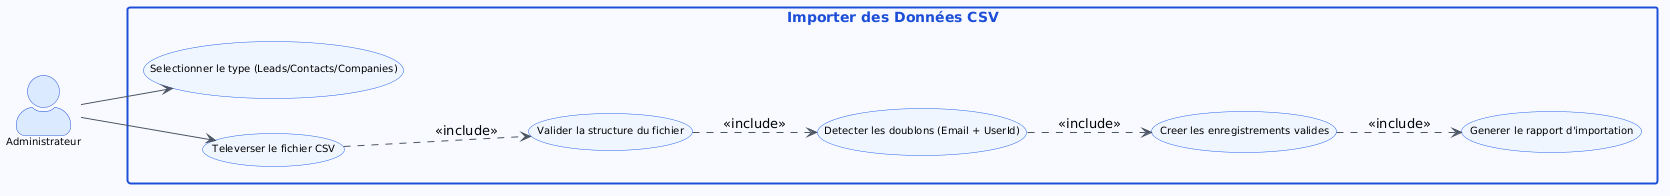
\includegraphics[width=0.8\textwidth]{images/uc_import.png}
    \caption{Diagramme de cas d’utilisation relatif à « Importer des Données »}
    \label{fig:uc_importer_donnees}
\end{figure}

\section{Diagrammes de séquence système}

Les schémas de séquence système fournissent une illustration dans l’ordre temporel des interactions entre les composants du système. Ils décrivent les interactions entre l’utilisateur, le frontend Next.js, le backend NestJS et les services tiers.

\subsection{Diagramme de séquence système relatif au cas d’utilisation « S’authentifier »}

La figure 2.6 présente le schéma du processus d’authentification d’un utilisateur. L’utilisa-
teur saisit ses informations de connexion dans le formulaire d’accès. Le backend NestJS exa-
mine l’existence du compte dans la base de données MySQL, compare le mot de passe saisi avec le hash Bcrypt enregistré, puis crée et renvoie un token JWT signé. Ce token est par la suite conservé dans les cookies sécurisés du navigateur et associé à chaque demande API sui-
vante.

\begin{figure}[H]
    \centering
    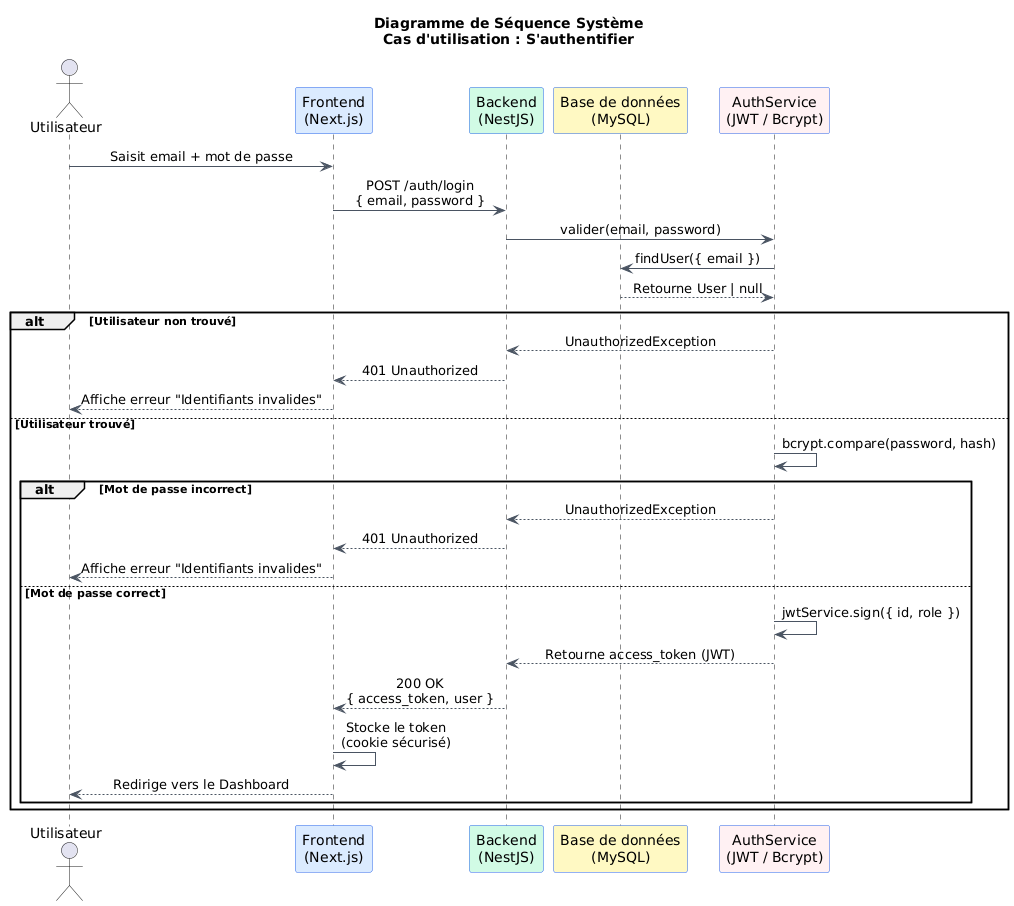
\includegraphics[width=\textwidth]{images/seq_authentification.png}
    \caption{Diagramme de séquence système relatif au cas d’utilisation « S’authentifier »}
    \label{fig:ss_authentifier}
\end{figure}

\subsection{Diagramme de séquence système relatif au cas d’utilisation « Calculer le Score IA »}

Le schéma de la figure 2.7 illustre l’interaction temporelle entre le frontend, le backend NestJS et le micro-service Python FastAPI en vue d’obtenir une prévision de conversion. Le backend puise les caractéristiques appropriées de la base de données et les transmet en POST à l’endpoint /predict-score. Si l’agent d’IA donne une réponse adéquate, le score, la catégorie ainsi que les motifs explicatifs sont sauvegardés et renvoyés à l’interface utilisateur. Si une erreur ou un dépassement de délai se produit, un score de repli calculé par le moteur des règles est renvoyé.

\begin{figure}[H]
    \centering
     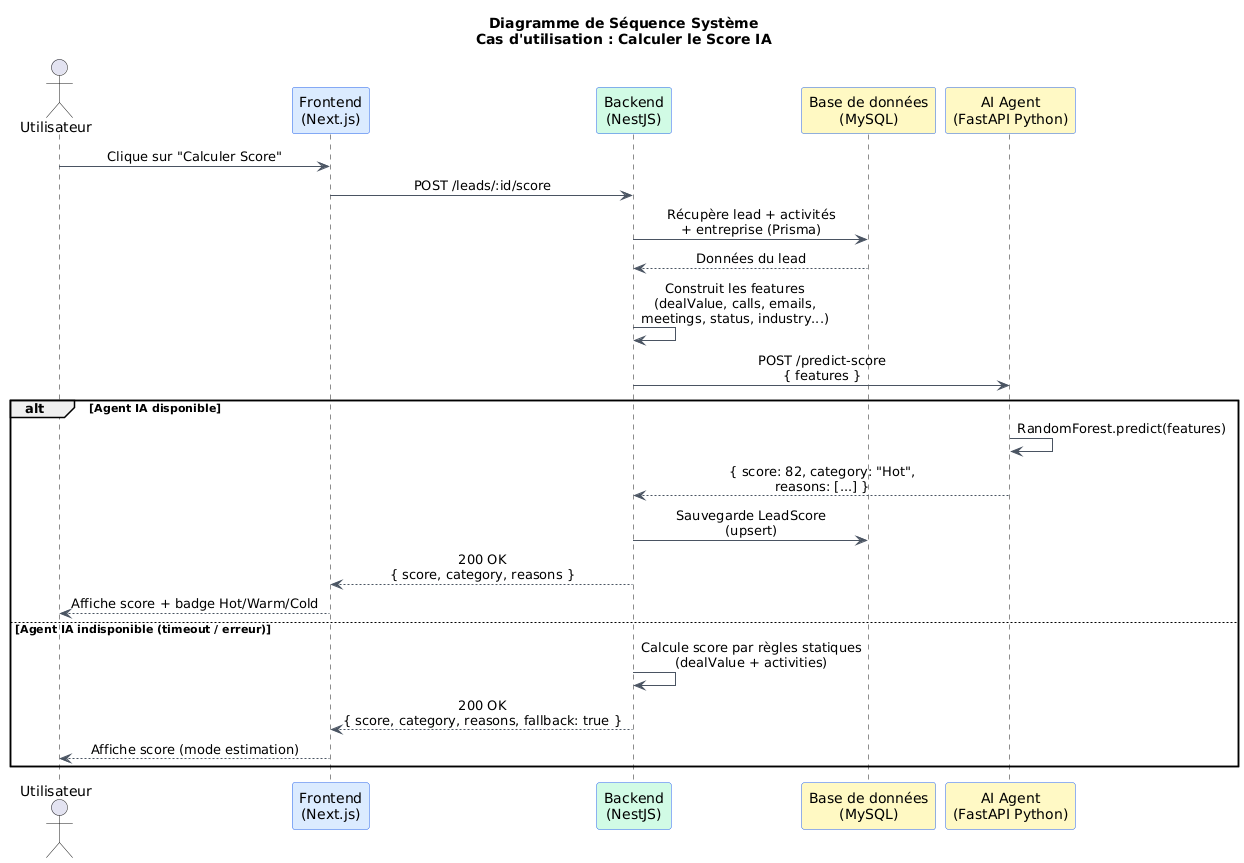
\includegraphics[width=\textwidth]{images/seq_scoring.png}
    \caption{Diagramme de séquence système relatif au cas d’utilisation « Calculer le Score IA »}
    \label{fig:ss_calculer_score_ia}
\end{figure}

\subsection{Diagramme de séquence système relatif au cas d’utilisation « Générer Email avec Gemini »}

Le schéma de la figure 2.8 représente la séquence de communication pour l’élaboration d’un projet d’email sur mesure. Le backend NestJS assemble l’intégralité du contexte du prospect (annotations, historique, évaluation IA), élabore une invite organisée pour l’API Google Gemini et restitue le contenu produit sous la forme d’un projet modifiable. En cas d’indisponibilité de l’API, le module de fallback produit un modèle sur mesure en fonction du statut et de la température du lead.

\begin{figure}[H]
    \centering
     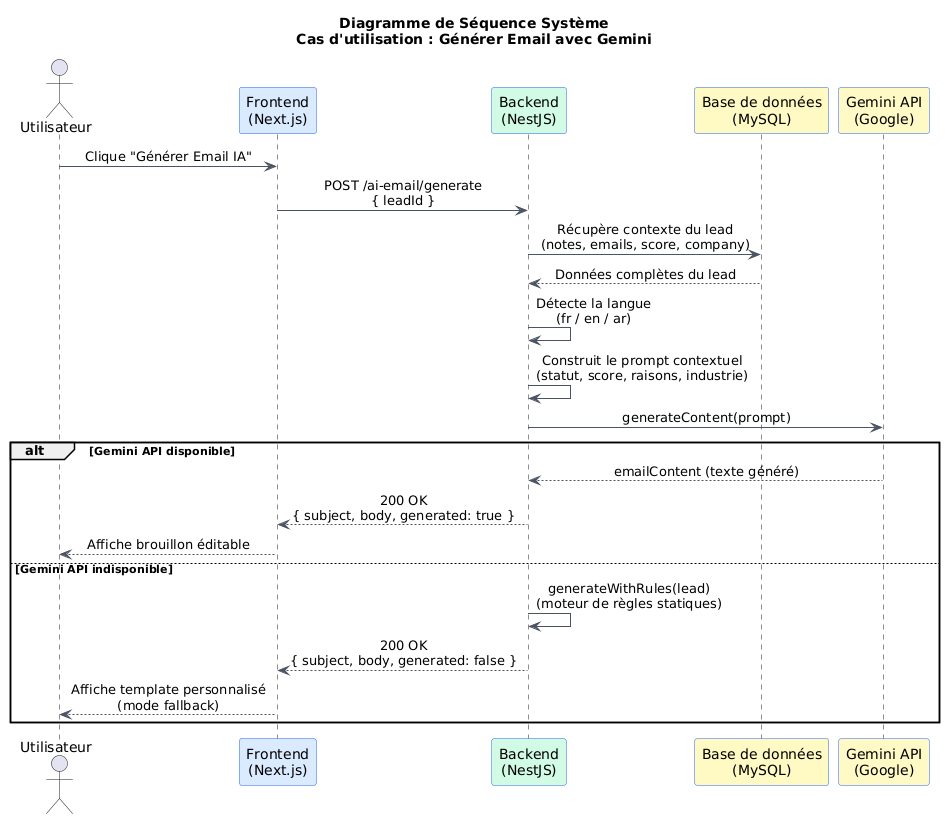
\includegraphics[width=\textwidth]{images/seq_gemini.png}
    \caption{Diagramme de séquence système relatif au cas d’utilisation « Générer Email via Gemini »}
    \label{fig:ss_generer_email}
\end{figure}

\subsection{Diagramme de séquence système relatif au cas d’utilisation « Importer des Données CSV »}

Le processus d’importation de données en grande quantité est illustré par le diagramme de la figure 2.9. Un fichier CSV est téléchargé par l’administrateur à travers l’interface. Le backend NestJS analyse le fichier, gère chaque ligne dans l’ordre en s’assurant que les champs requis sont remplis, contrôle la singularité à travers une opération d’« upset » sur la clé composite (Email + UserId) et produit un rapport final récapitulatif.

\begin{figure}[H]
    \centering
    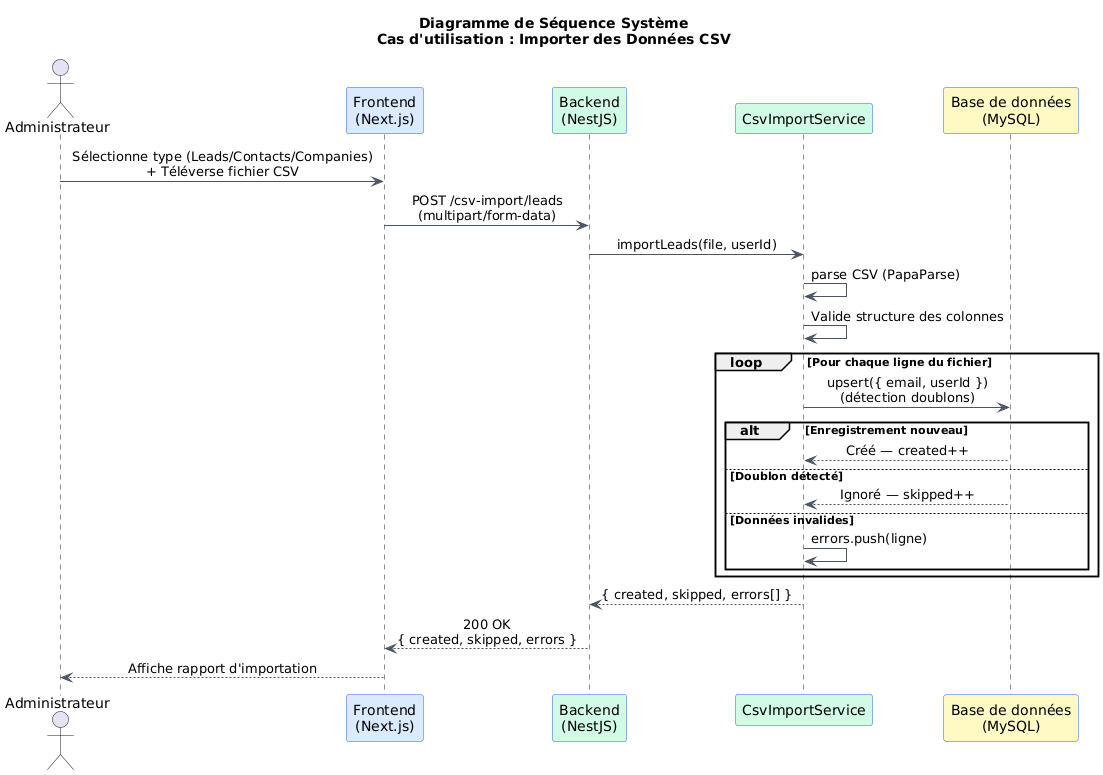
\includegraphics[width=\textwidth]{images/seq_import_csv.png}
    \caption{Diagramme de séquence système relatif au cas d’utilisation « Importer des Données CSV »}
    \label{fig:ss_importer_csv}
\end{figure}

\section*{Conclusion}

Dans ce chapitre, nous avons commencé par identifier les intervenants de notre système, à savoir le Représentant Commercial, l’Administrateur, l’API Gemini et le micro-service de scoring IA, en précisant leurs fonctions et obligations respectives. Par la suite, nous avons mi-
nutieusement défini les exigences fonctionnelles, englobant tous les modules du CRM, ainsi que les exigences non fonctionnelles liées à la sécurité, à la performance, à la disponibilité et à la facilité de maintenance. Finalement, nous avons introduit une modélisation UML organisée en packages, incluant des diagrammes de cas d’utilisation par acteur, des diagrammes détaillés par fonctionnalité et des diagrammes de séquence système relatifs aux processus critiques. Le prochain chapitre se focalisera sur la conception architecturale et les décisions technologiques prises pour l’implémentation de cette solution.
\clearpage

% Chapitre 3 (page 10)
\chapter{Aperçu conceptuel et Conception détaillée}
\label{chap:conception}

\section*{Introduction}
\addcontentsline{toc}{section}{Introduction}

La phase de conception est une étape très importante dans le cycle de développement de notre CRM intelligent. Tout d’abord, nous devons clarifier la vision globale de l’architecture. Ensuite, nous devons décrire en détail la conception de chaque module. Cette description comprend les vues statiques, qui sont présentées via le diagramme de classes d’entités, et les vues dynamiques, qui détaillent le fonctionnement interne de l’application à travers les diagrammes de séquences de conception et les diagrammes de classes participantes. L’objectif principal de la phase de conception est de transformer les spécifications établies dans le chapitre précédent en modèles techniques clairs. Cela prépare le terrain pour la phase de réalisation de notre CRM intelligent.

%──────────────────────────────────────────────────────
\section{Architecture physique et logique}
%──────────────────────────────────────────────────────

\subsection{Architecture 3-tiers orientée services}

Nous avons choisi, pour la conception de notre solution CRM Micro-SaaS, une architecture basée sur le modèle à 3 niveaux, complétée par une approche de micro-services pour intégrer l’intelligence artificielle. Ce modèle logique a pour but de dissocier clairement les responsabilités au sein du système. Cette architecture comporte trois niveaux que l'on peut décrire brièvement comme suit :
\begin{itemize}
    \item \textbf{Couche présentation (Frontend) :} Il s'agit de la partie de l'application que l'utilisateur voit et avec laquelle il interagit. Elle est développée avec \textbf{Next.js} et React, et offre une interface dynamique, réactive et sécurisée.
    \item \textbf{Couche applicative (Backend et Services IA) :} C’est le cerveau de l’application. Elle contient la logique métier et les règles de gestion, et traite toutes les requêtes des utilisateurs. Cette couche est constituée de deux éléments principaux : le serveur principal en \textbf{NestJS} qui gère les entités du CRM, et un micro-service en \textbf{FastAPI} dédié exclusivement au \textit{lead scoring} par intelligence artificielle.
    \item \textbf{Couche d’accès aux données :} C’est la couche responsable de la persistance des données. Elle utilise le système de gestion de bases de données relationnelles \textbf{MySQL} et l’ORM \textbf{Prisma} pour garantir la sécurité et la cohérence des données lors des opérations de lecture et d’écriture.
\end{itemize}

\begin{figure}[H]
    \centering
     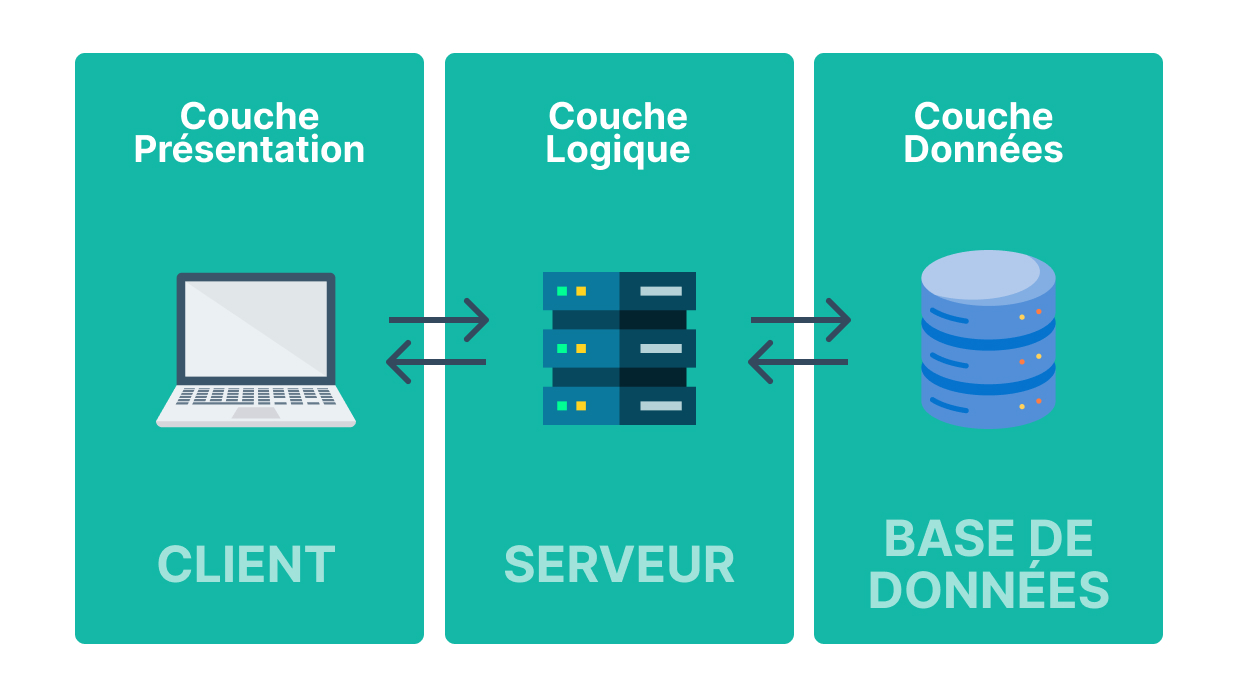
\includegraphics[width=\textwidth,height=0.82\textheight,keepaspectratio]{images/architecture_3tiers.png}
    \caption{Architecture globale de l'application (Image manquante)}
    \label{fig:architecture_globale}
\end{figure}

%──────────────────────────────────────────────────────
\section{Patrons de conception}
%──────────────────────────────────────────────────────

Lors du développement d'applications complexes comme un CRM, nous faisons souvent face à certains problèmes de conception récurrents. Pour les résoudre de manière efficace et réutilisable, nous utilisons des patrons de conception (\textit{Design Patterns}). Ce sont des modèles reconnus permettant non seulement de résoudre un problème, mais aussi d’améliorer la qualité du code, sa maintenabilité et d’accélérer le processus de développement.

\subsection{Patron de conception MVC (Modèle-Vue-Contrôleur)}

Le \textit{Model-View-Controller} (MVC) est l’un des patrons de conception les plus utilisés pour le développement web. Bien que physiquement réparti entre le frontend et le backend dans notre système moderne, son principe conceptuel régit notre application :
\begin{itemize}
    \item \textbf{Modèle :} Géré par Prisma et NestJS, il représente les données pures de l’application (Leads, Contacts, Deals, etc.) et encapsule la logique de manipulation des données.
    \item \textbf{Vue :} Gérée par Next.js à travers des composants React (TailwindCSS, Shadcn UI), elle permet de présenter et de mettre en forme les données du modèle pour l’utilisateur final de façon réactive.
    \item \textbf{Contrôleur :} Implémenté via les contrôleurs NestJS et les Server Actions de Next.js, il se place entre la vue et le modèle. Il intercepte les requêtes de l'utilisateur, sollicite les services adéquats et retourne la réponse formatée.
\end{itemize}

\begin{figure}[H]
    \centering
     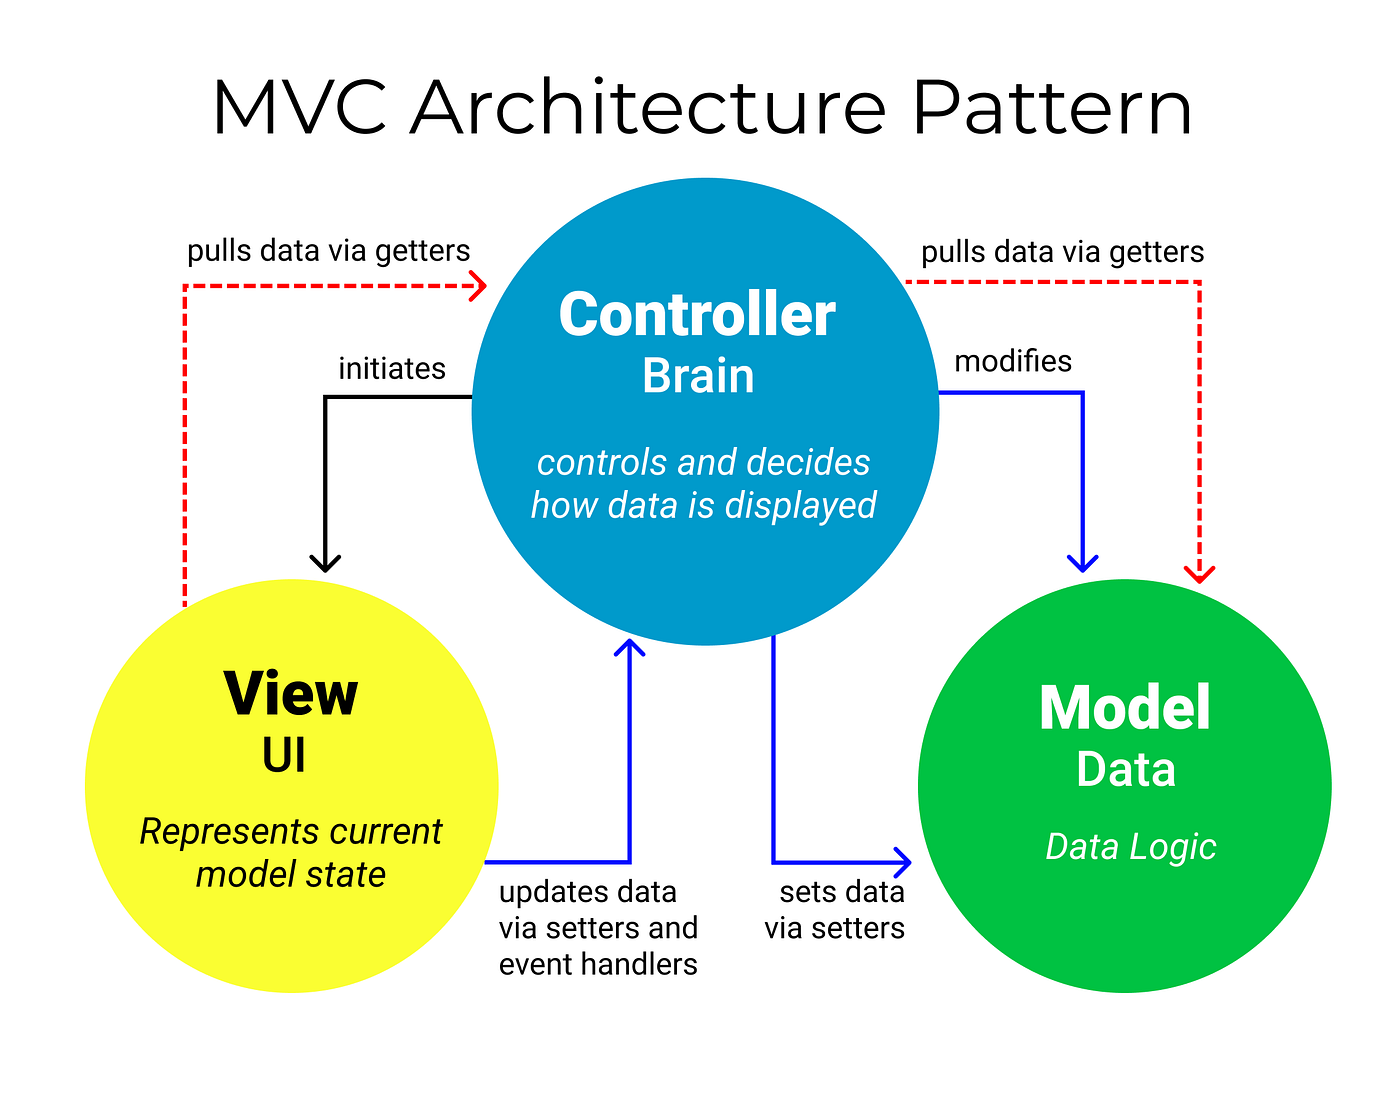
\includegraphics[width=0.95\textwidth,height=0.78\textheight,keepaspectratio]{images/patron_mvc.png}
    \caption{Principe du patron de conception MVC dans l'application (Image manquante)}
    \label{fig:patron_mvc}
\end{figure}

\subsection{Patron de conception DAO (Data Access Object) / Repository}

Le patron de conception DAO permet de séparer la logique métier de la logique d’accès aux données. Dans notre projet, le rôle de DAO est assuré de manière moderne par \textbf{Prisma Client}. 

Les objets de données sont représentés par des modèles (schémas Prisma), qui sont généralement simples et ne contiennent que les informations de la base. Les services NestJS utilisent les méthodes fournies par l'ORM pour effectuer les opérations CRUD sans écrire de requêtes SQL brutes, assurant ainsi une abstraction sécurisée de la source de données.

\begin{figure}[H]
    \centering
    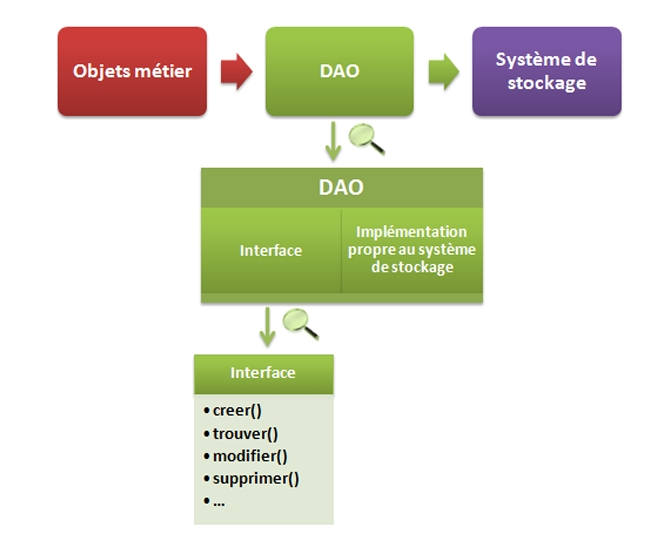
\includegraphics[width=0.95\textwidth,height=0.78\textheight,keepaspectratio]{images/patron_dao.png}
    \caption{Principe du patron de conception DAO avec Prisma (Image manquante)}
    \label{fig:patron_dao}
\end{figure}

\subsection{Patron de conception DTO (Data Transfer Object)}

Le patron de conception DTO est un modèle qui permet de séparer la logique métier de l’application de la logique de transfert de données. Le principe de ce patron est de créer une classe qui contient les données que l’on souhaite transférer, sans comportement métier associé.

Dans notre architecture NestJS, les DTOs sont utilisés pour encapsuler les données et les transférer entre le client et le backend. Décorés avec \textit{class-validator}, ils garantissent que seules les données valides, typées et autorisées transitent sur le réseau, sécurisant ainsi les endpoints de l'API.

\begin{figure}[H]
    \centering
    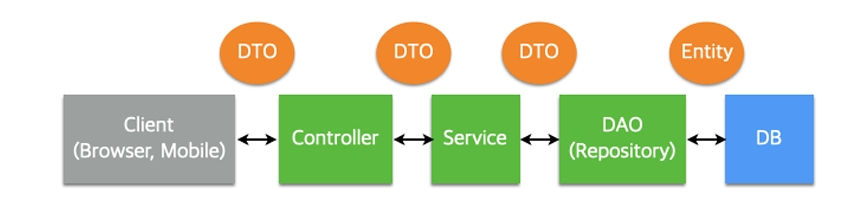
\includegraphics[width=0.95\textwidth,height=0.78\textheight,keepaspectratio]{images/patron_dto.png}
    \caption{Principe du patron de conception DTO}
    \label{fig:patron_dto}
\end{figure}

%──────────────────────────────────────────────────────
\section{Conception détaillée}
%──────────────────────────────────────────────────────

Afin d’avoir une vue claire et approfondie sur la structure interne du système, nous allons présenter en premier lieu le diagramme de classes des entités de la solution entière. Ensuite, nous exposerons la conception détaillée des modules principaux à l’aide des diagrammes de classes participantes et des diagrammes de séquences de conception.

\subsection{Diagramme de classe d’entités}

Ce diagramme est souvent considéré comme le diagramme le plus important dans la modélisation orientée-objet. Il s’agit d’une représentation statique des éléments constituant un système avec leurs attributs et leurs opérations ainsi que les différentes relations entre eux.

Le modèle conceptuel de données de notre CRM gravite autour d'entités centrales structurant l'activité commerciale : \texttt{User}, \texttt{Company}, \texttt{Contact}, \texttt{Lead}, \texttt{Deal}, \texttt{Task} et \texttt{Ticket}.

\begin{figure}[H]
    \centering
    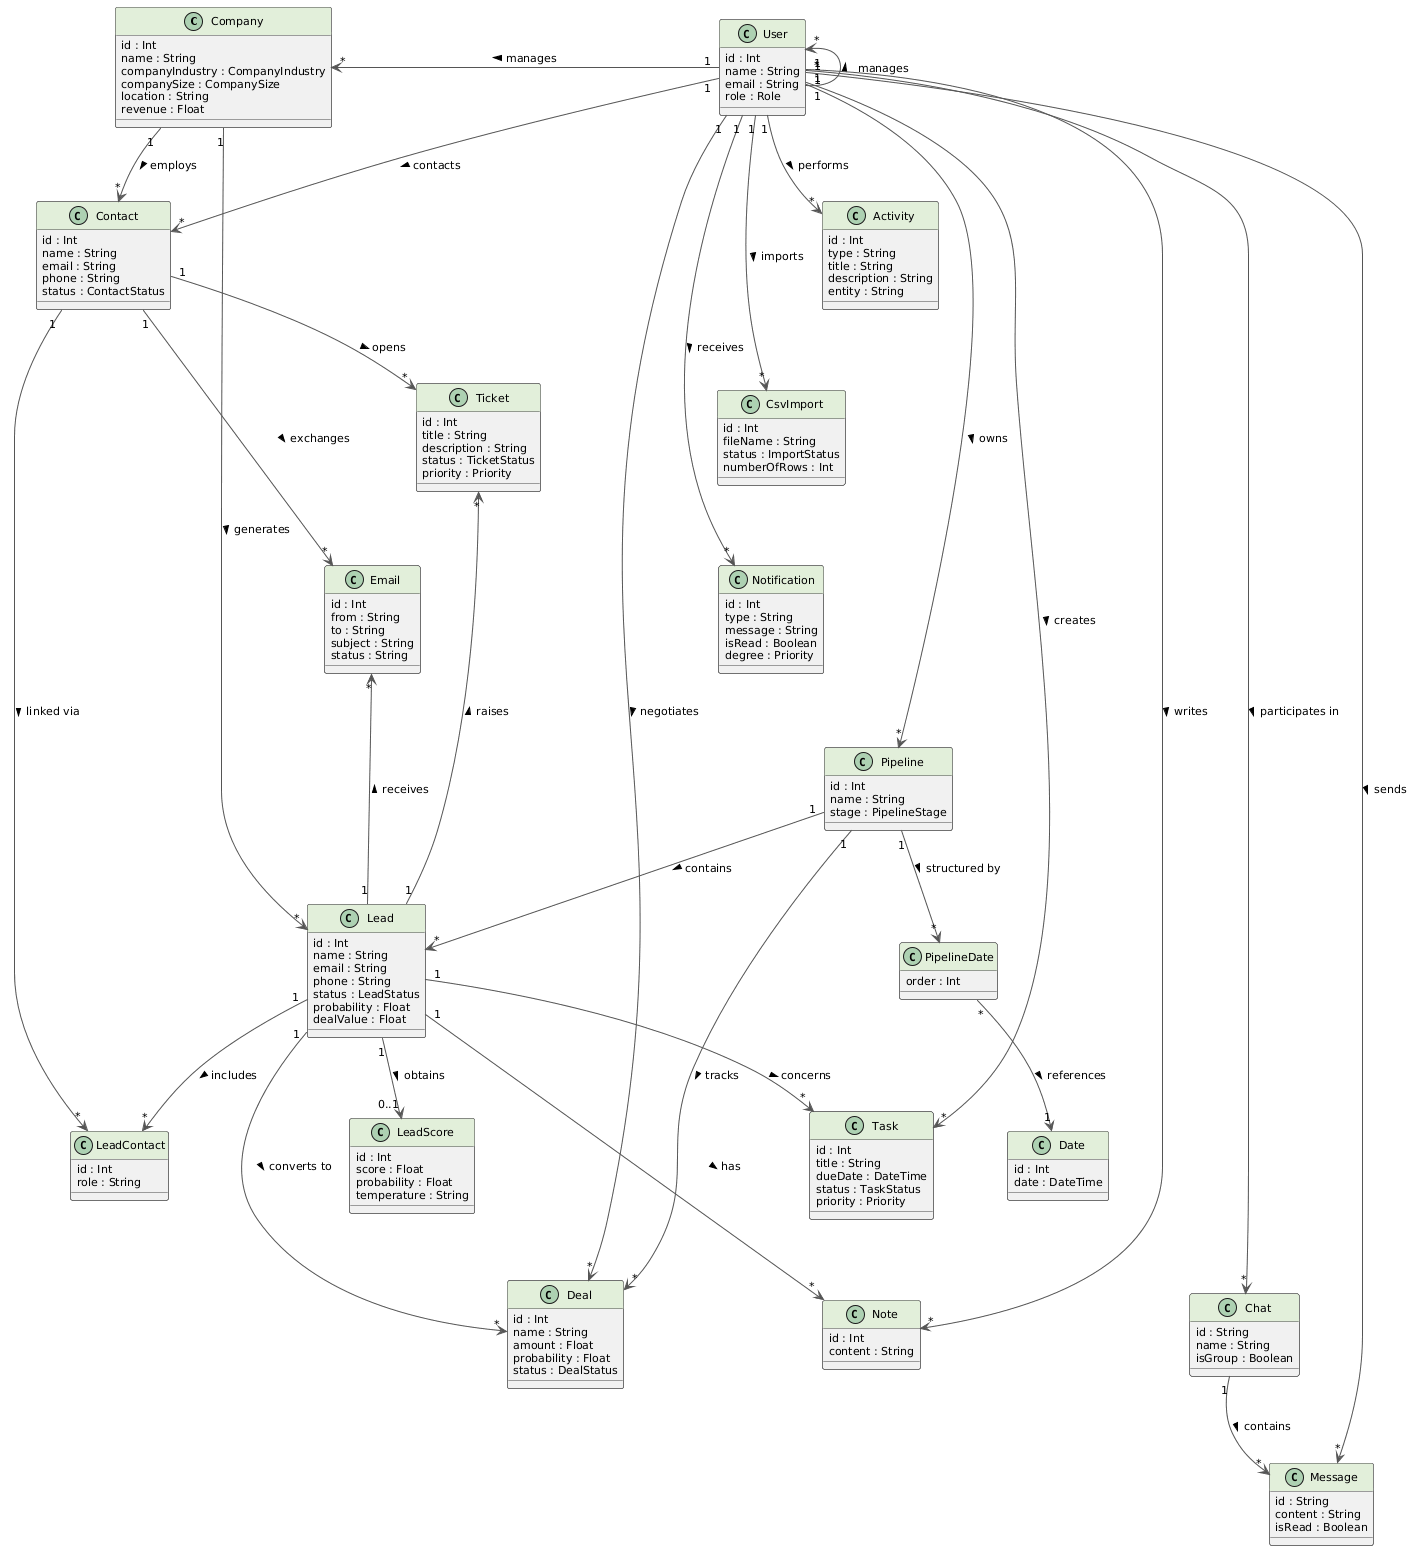
\includegraphics[width=\textwidth,height=0.86\textheight,keepaspectratio]{images/diagramme_classes_entites.png}
    \caption{Diagramme de classe d'entités du CRM}
    \label{fig:diagramme_classes}
\end{figure}

\begin{figure}[H]
    \centering
    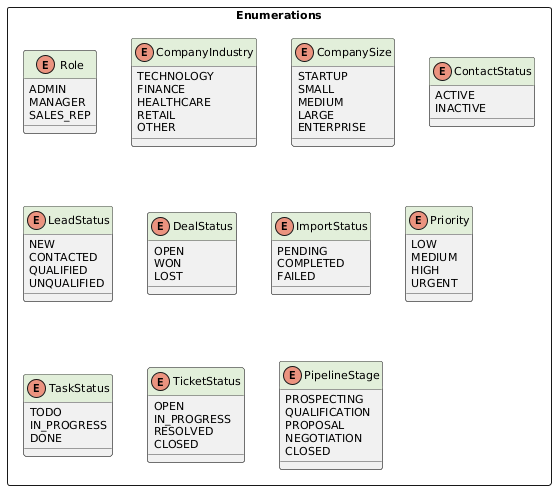
\includegraphics[width=\textwidth,height=0.82\textheight,keepaspectratio]{images/diagramme_classes_enumerations.png}
    \caption{Énumérations utilisées dans le modèle de données}
    \label{fig:diagramme_enumerations}
\end{figure}

\subsection{Diagrammes de séquences de conception (DSC)}

Les diagrammes de séquences permettent de modéliser comment les éléments internes du système interagissent entre eux selon un point de vue chronologique, en dévoilant l'appel des méthodes entre les contrôleurs, les services, et la base de données.

\subsubsection{Diagramme de séquence de conception \og~S'authentifier~\fg{}}

Lorsqu'un utilisateur tente de se connecter, le contrôleur d'authentification (\texttt{AuthController}) réceptionne la requête. Il fait appel au \texttt{AuthService} qui, à son tour, vérifie l'existence du compte via le \texttt{UsersService} et valide le hachage du mot de passe. Si le mot de passe correspond, un jeton d'accès JWT est généré et retourné pour être stocké dans le navigateur.

\begin{figure}[H]
    \centering
    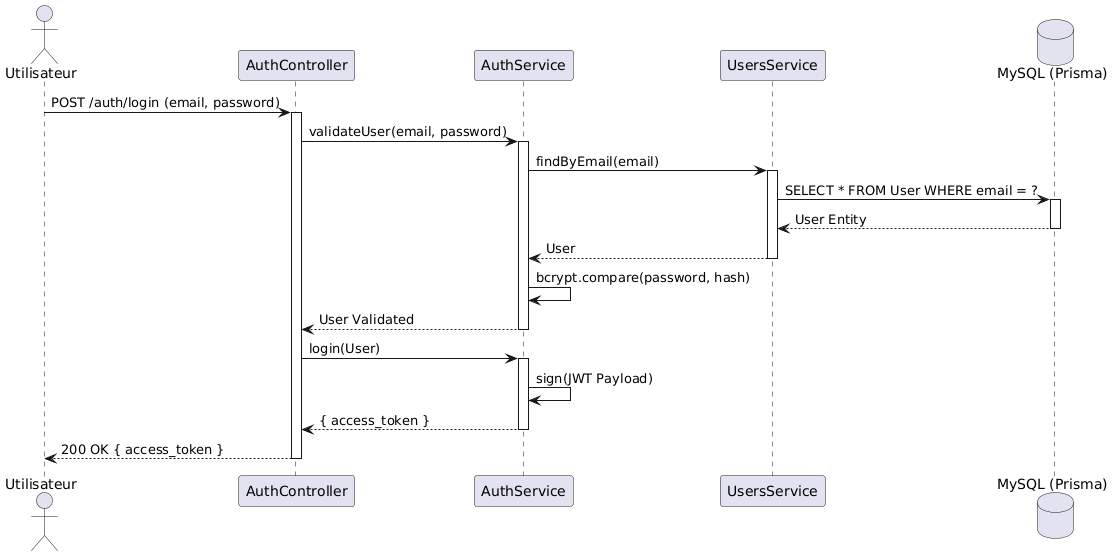
\includegraphics[width=\textwidth,height=0.82\textheight,keepaspectratio]{images/dsc_authentification.png}
    \caption{Diagramme de séquence de conception \og~S'authentifier~\fg{}}
    \label{fig:dsc_auth}
\end{figure}

\subsubsection{Diagramme de séquence de conception \og~Calculer Score IA (Lead Scoring)~\fg{}}

Pour évaluer la probabilité de conversion d'un prospect, le système interagit avec le micro-service IA. Le \texttt{LeadsController} invoque le \texttt{LeadsService}, qui assemble les données pertinentes du lead. Ces données sont expédiées par requête HTTP POST au \texttt{FastAPI AI Agent}. L'agent retourne un score calculé par son modèle d'apprentissage automatique. Le \texttt{LeadsService} met alors à jour l'entité \texttt{Lead} via Prisma et retourne le résultat complet.

\begin{figure}[H]
    \centering
    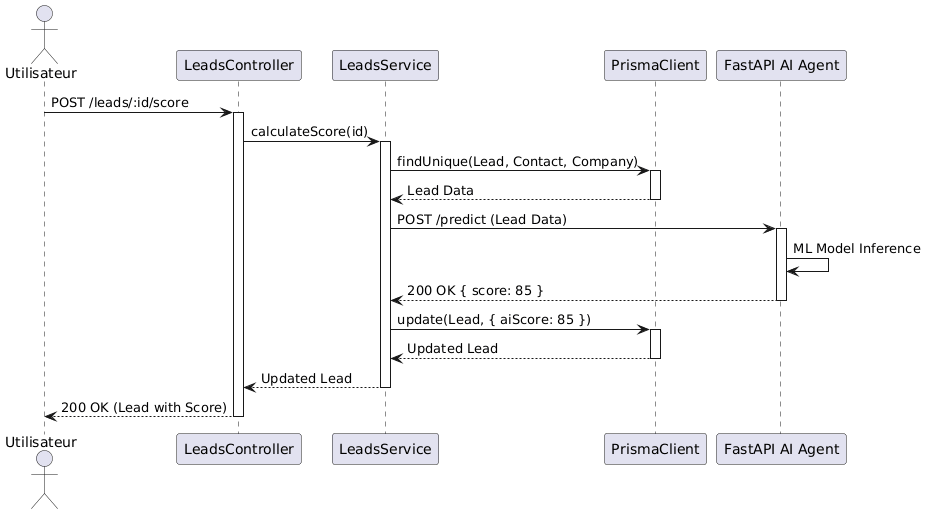
\includegraphics[width=\textwidth,height=0.82\textheight,keepaspectratio]{images/dsc_scoring_ia.png}
    \caption{Diagramme de séquence de conception \og~Calculer Score IA~\fg{}}
    \label{fig:dsc_scoring}
\end{figure}

\subsubsection{Diagramme de séquence de conception \og~Générer Email avec Gemini~\fg{}}

L'utilisateur (Sales Rep) demande la génération d'un email d'approche pour un lead spécifique. La requête atteint le composant \texttt{AiEmailModal} puis le backend. Le \texttt{AiService} rassemble le contexte complet (informations du lead, entreprise, score) et soumet un \textit{prompt} formaté à l'API Google Gemini. La réponse générée est retransmise au client pour relecture et édition avant envoi.

\begin{figure}[H]
    \centering
    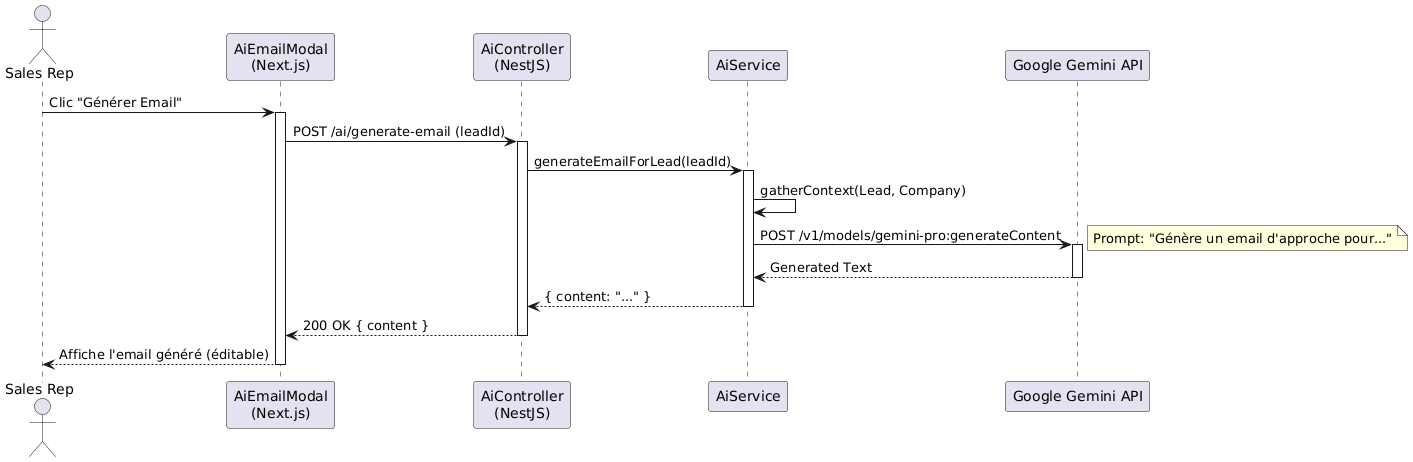
\includegraphics[width=\textwidth,height=0.82\textheight,keepaspectratio]{images/dsc_gemini_email.png}
    \caption{Diagramme de séquence de conception \og~Générer Email avec Gemini~\fg{}}
    \label{fig:dsc_gemini}
\end{figure}

\subsection{Diagramme de classes participantes (DCP)}

Le diagramme de classes participantes (DCP) fait le lien entre les cas d’utilisation, l'interface utilisateur et les diagrammes de conception logicielle. Il modélise les classes de dialogue (les composants Next.js), les classes de contrôle (les Services et Contrôleurs NestJS) et les entités (les Modèles Prisma).

\subsubsection{DCP du cas d'utilisation \og~Gérer les Leads~\fg{}}

Dans ce diagramme, nous observons l’interaction des composants d'interface (\texttt{LeadsTable}, \texttt{LeadDetailsModal}) avec le contrôleur \texttt{LeadsController}. Ce dernier interroge et modifie les informations en faisant appel au \texttt{LeadsService}, qui s'occupe de persister ou de récupérer les entités \texttt{Lead}, \texttt{Contact} et \texttt{Company} dans la base de données.

\begin{figure}[H]
    \centering
    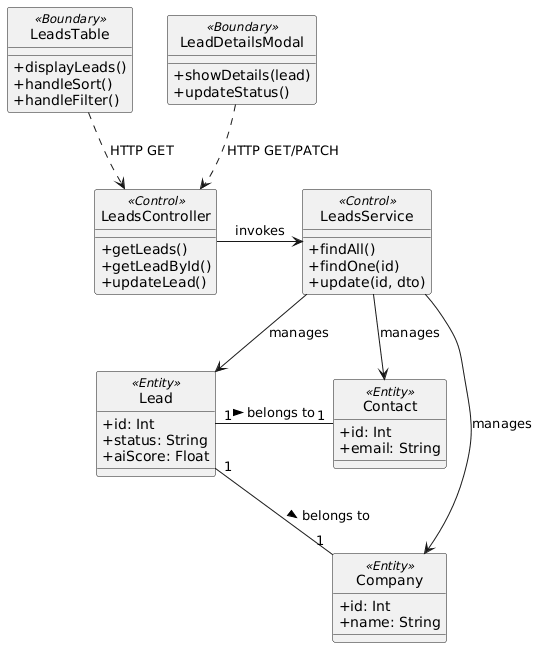
\includegraphics[width=\textwidth,height=0.82\textheight,keepaspectratio]{images/dcp_gerer_leads.png}
    \caption{DCP du cas d'utilisation \og~Gérer les Leads~\fg{}}
    \label{fig:dcp_leads}
\end{figure}

\subsubsection{DCP du cas d'utilisation \og~Importer Données CSV~\fg{}}

Ce diagramme illustre la communication entre le composant d'importation \texttt{CSVImportWizard} et les contrôleurs backend correspondants. Le \texttt{ImportService} réceptionne et analyse le fichier, manipule les \texttt{CreateContactDto} ou \texttt{CreateLeadDto}, effectue la validation, et insère les entités résultantes dans la base pour traiter les données en masse.

\begin{figure}[H]
    \centering
    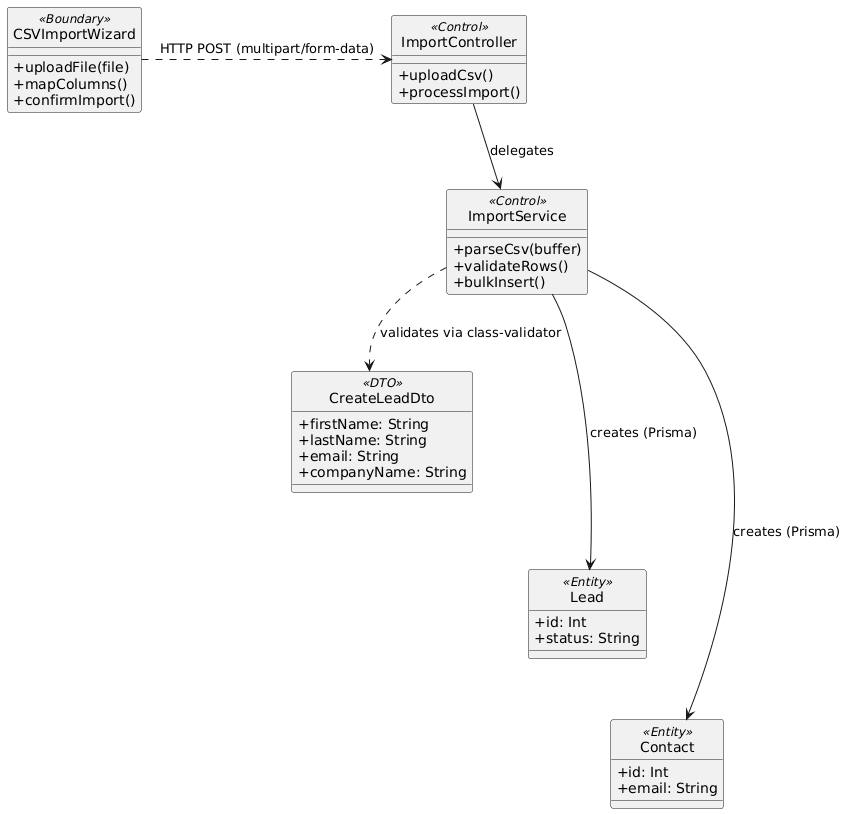
\includegraphics[width=\textwidth,height=0.82\textheight,keepaspectratio]{images/dcp_import_csv.png}
    \caption{DCP du cas d'utilisation \og~Importer Données CSV~\fg{}}
    \label{fig:dcp_import}
\end{figure}

\subsection{Diagramme de blocs internes}

Le diagramme de blocs internes offre une vue d'ensemble de la hiérarchie et de la distribution des responsabilités au sein des différents niveaux de notre système. Inspiré par les architectures en couches robustes, ce modèle illustre l'intégration entre la couche de présentation (les composants d'interface), la logique applicative (les contrôleurs et les services) et la logique métier (les entités de la base de données). Il met en évidence la fluidité de la communication verticale, depuis l'interaction de l'utilisateur jusqu'à la persistance des données.

\begin{figure}[H]
    \centering
    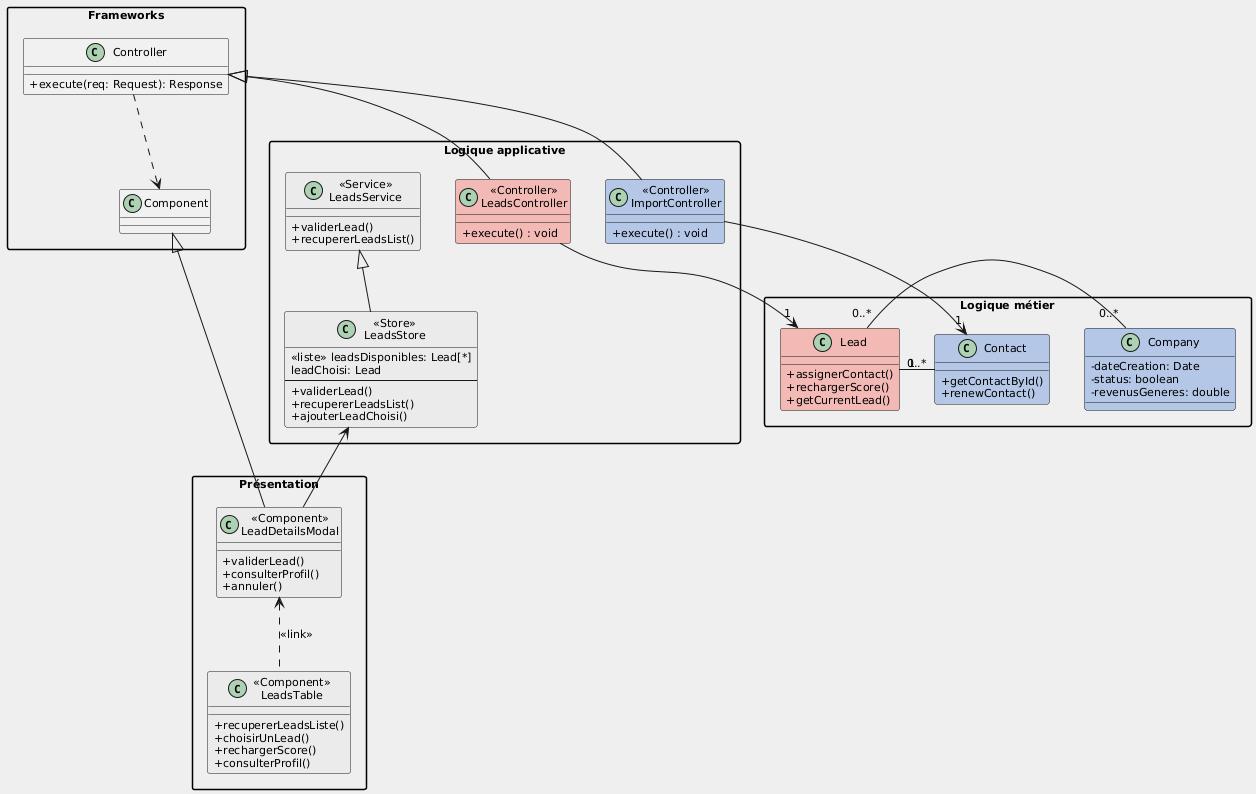
\includegraphics[width=\textwidth,height=0.82\textheight,keepaspectratio]{images/diagramme_blocs_internes.png}
    \caption{Diagramme de blocs internes du système}
    \label{fig:diagramme_blocs_internes}
\end{figure}

%──────────────────────────────────────────────────────
\section*{Conclusion}
\addcontentsline{toc}{section}{Conclusion}
%──────────────────────────────────────────────────────

Ce chapitre a permis de passer de la vision fonctionnelle abstraite à une perspective technique et conceptuelle précise. L'architecture orientée services adoptée, qui combine Next.js, NestJS et FastAPI, fournit une séparation nette des responsabilités, modélisée selon l'approche 3-tiers. L'utilisation de patrons de conception standards de l'industrie (MVC, DAO, DTO) garantit une base de code maintenable, sécurisée et pérenne. Par l'élaboration des diagrammes de classes (structure statique) et de séquences (comportement dynamique), nous avons pu dresser une cartographie complète du fonctionnement interne du logiciel. L'application est dorénavant prête pour la phase d'implémentation, qui sera abordée dans le chapitre suivant.

\clearpage

% Chapitre 4 (page 11)
\chapter{Réalisation}

\section*{Introduction}
Dans ce chapitre, nous débutons par décrire l'environnement de travail en mentionnant les technologies et les outils que nous avons utilisés. Ensuite, nous présentons l'architecture de déploiement de notre solution. Enfin, nous concluons en présentant les différentes interfaces Homme/Machine que nous avons développées.

%% ============================================================
%%  4.1  DIAGRAMME DE DÉPLOIEMENT
%% ============================================================
\section{Diagramme de déploiement}

Dans ce qui suit, nous décrivons l'architecture logicielle de notre plateforme CRM à travers le diagramme de déploiement présenté ci-dessous par la figure~\ref{fig:deploiement}.

\begin{figure}[H]
    \centering
    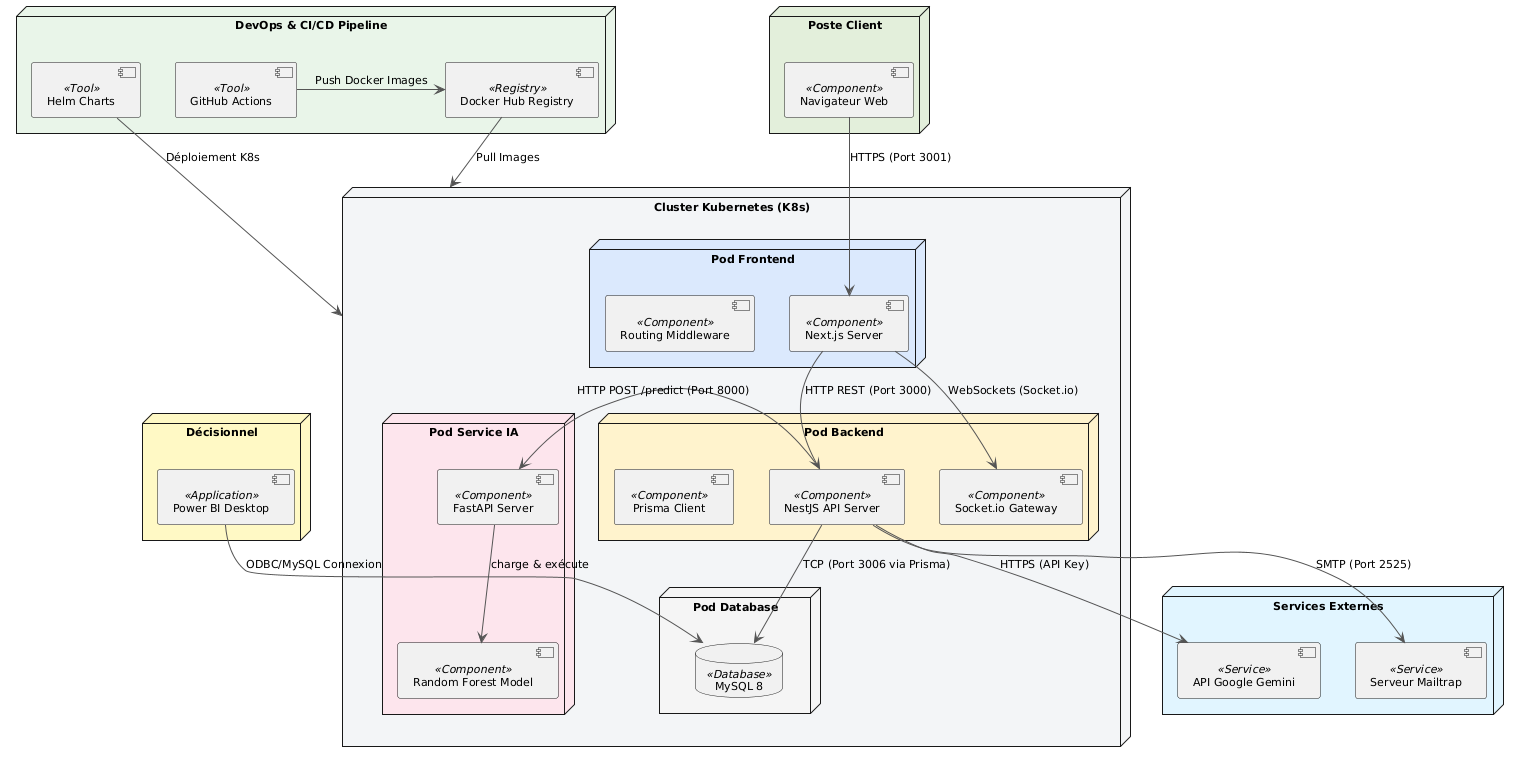
\includegraphics[width=\textwidth,height=0.82\textheight,keepaspectratio]{images/diagramme_deploiement.png}
    \caption{Diagramme de déploiement}
    \label{fig:deploiement}
\end{figure}

Le tableau~\ref{tab:composants} décrit les différents composants matériels et logiciels de notre système.

\begin{table}[H]
\centering
\renewcommand{\arraystretch}{1.4}
\begin{tabular}{|p{3.5cm}|p{10cm}|}
\hline
\textbf{Nom} & \textbf{Description} \\
\hline
Next.js (Frontend) & Framework React pour le rendu côté serveur et la génération de pages statiques, servant l'interface utilisateur de la plateforme CRM. \\
\hline
NestJS (Backend) & Framework Node.js progressif pour la construction d'API REST efficaces et évolutives, gérant la logique métier et l'accès aux données. \\
\hline
FastAPI (AI Agent) & Framework Python haute performance pour la construction du microservice d'intelligence artificielle dédié au scoring des leads. \\
\hline
MySQL & Système de gestion de base de données relationnelle utilisé pour le stockage persistant de toutes les données de l'application. \\
\hline
Prisma ORM & Outil de mapping objet-relationnel (ORM) moderne pour Node.js et TypeScript, facilitant les interactions avec la base de données MySQL. \\
\hline
Docker & Plateforme de conteneurisation permettant d'encapsuler chaque service dans un conteneur isolé et reproductible. \\
\hline
Docker Compose & Outil d'orchestration multi-conteneurs permettant de définir et gérer l'ensemble des services de la plateforme. \\
\hline
Kubernetes (K8s) & Système d'orchestration de conteneurs pour le déploiement, la mise à l'échelle et la gestion automatisée des applications conteneurisées. \\
\hline
Helm & Gestionnaire de packages pour Kubernetes, simplifiant le déploiement et la gestion des charts applicatifs. \\
\hline
GitHub Actions & Service d'intégration et de déploiement continus (CI/CD) permettant d'automatiser le pipeline de build, test et déploiement. \\
\hline
Docker Hub & Registre d'images Docker utilisé pour stocker et distribuer les images conteneurisées de nos services. \\
\hline
Socket.io & Bibliothèque de communication en temps réel basée sur les WebSockets, utilisée pour le chat et les notifications en temps réel. \\
\hline
Power BI & Outil de Business Intelligence de Microsoft utilisé pour la création de tableaux de bord analytiques avancés. \\
\hline
Gemini AI & API d'intelligence artificielle générative de Google, utilisée pour la génération d'e-mails personnalisés et pour propulser le chatbot intelligent avec approche RAG. \\
\hline
\end{tabular}
\caption{Description des composants matériels et logiciels du système}
\label{tab:composants}
\end{table}

%% ============================================================
%%  4.2  STYLE ARCHITECTURAL
%% ============================================================
\section{Le style architectural}

\subsection{Partie front-end}

\subsubsection{Architecture MVC avec Next.js}

L'architecture de notre application front-end repose sur le pattern \textbf{MVC} (Model-View-Controller) adapté au framework Next.js à travers l'App Router. Cette architecture favorise une séparation claire des responsabilités, permettant une maintenance plus aisée et facilitant les tests unitaires.

\begin{itemize}
    \item \textbf{Modèle (Model)} : Le modèle est géré par les hooks personnalisés et le store Zustand. Il représente l'état de l'application et la logique d'accès aux données via les appels API vers le backend NestJS.
    \item \textbf{Vue (View)} : La vue est constituée des composants React (TSX) utilisant Radix UI pour les composants d'interface, TailwindCSS pour le style et Framer Motion pour les animations. Elle est responsable de l'affichage et de la gestion des interactions utilisateur.
    \item \textbf{Contrôleur (Controller)} : Le contrôleur est implémenté à travers les Server Components et les handlers d'événements dans les pages Next.js. Il orchestre la communication entre le modèle et la vue, gère la navigation via le middleware d'authentification et le routage basé sur les rôles (Admin/Rep).
\end{itemize}

\begin{figure}[H]
    \centering
    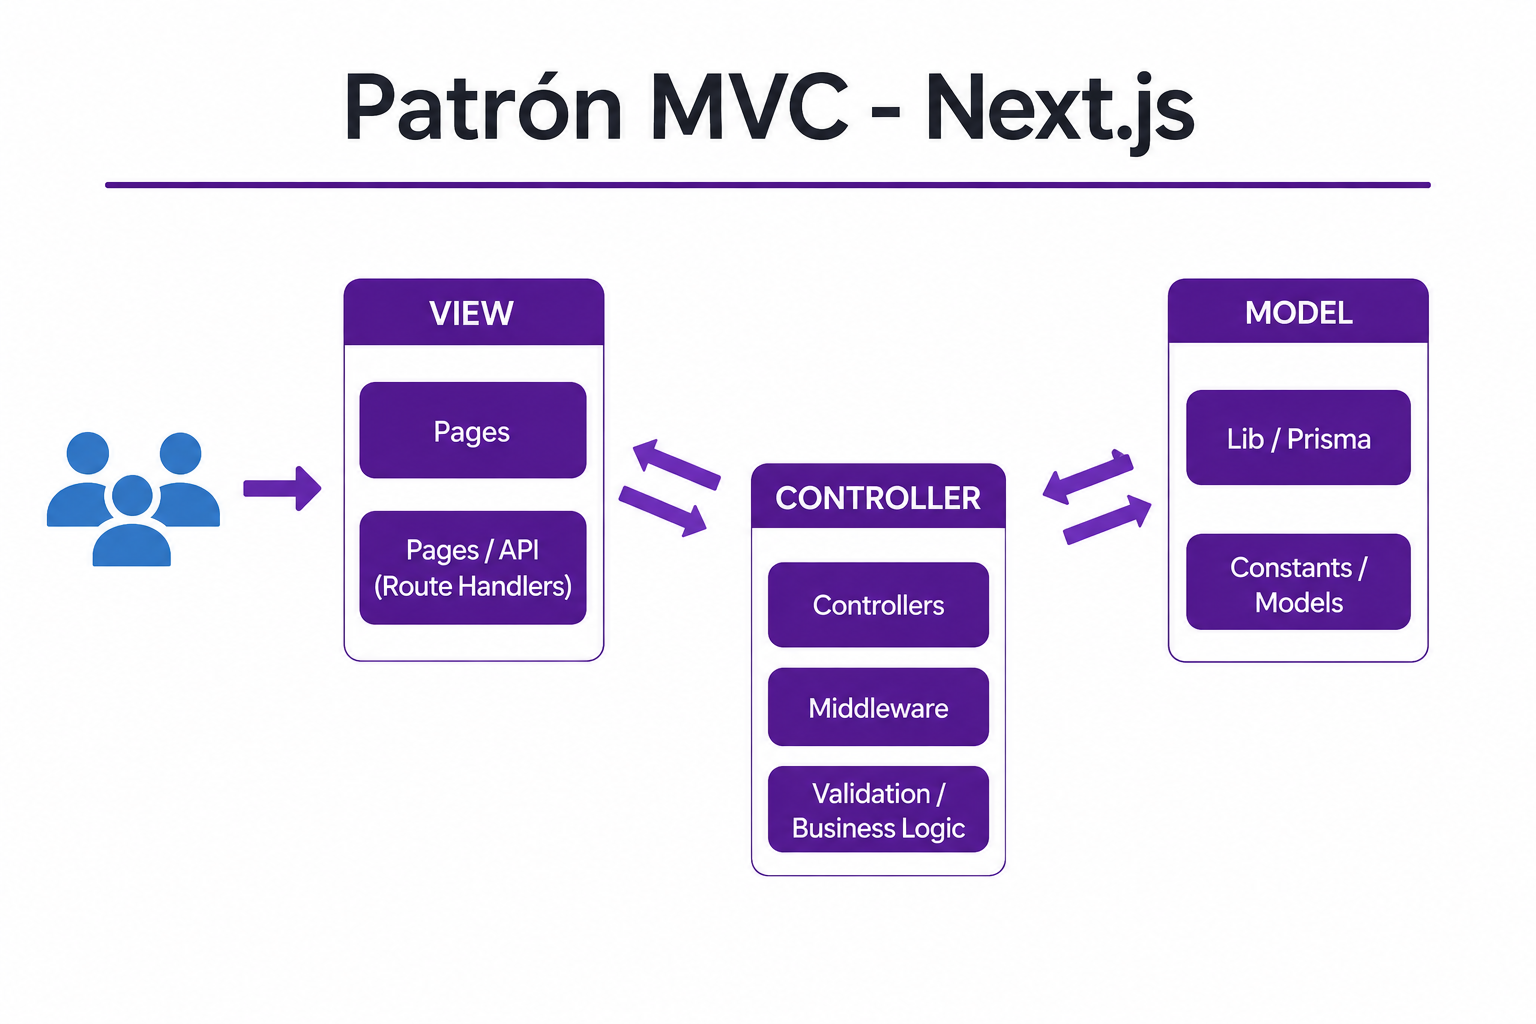
\includegraphics[width=\textwidth,height=0.82\textheight,keepaspectratio]{images/architecture_mvc_nextjs.png}
    \caption{Architecture MVC du front-end}
    \label{fig:mvc}
\end{figure}

\subsubsection{Diagramme de composants front-end}

Ce diagramme présente une vue d'ensemble de notre application web, illustrant les différents modules développés : le module d'authentification, les tableaux de bord Admin et Sales Rep, les modules de gestion (Leads, Contacts, Companies, Pipeline, Tickets), le module de chat en temps réel, ainsi que les intégrations avec l'API Gemini et le service de scoring IA.

\begin{figure}[H]
    \centering
    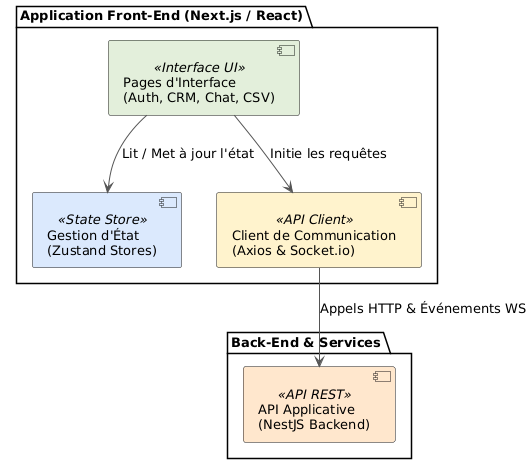
\includegraphics[width=\textwidth,height=0.82\textheight,keepaspectratio]{images/diagramme_composants_frontend.png}
    \caption{Diagramme de composants de l'application web}
    \label{fig:composants-frontend}
\end{figure}

\subsection{Partie back-end}

\subsubsection{Architecture Modulaire NestJS}

L'architecture back-end repose sur le framework \textbf{NestJS}, qui adopte une approche modulaire inspirée d'Angular. Chaque fonctionnalité métier est encapsulée dans un module indépendant contenant ses propres contrôleurs, services et DTOs (Data Transfer Objects). Cette architecture favorise :

\begin{itemize}
    \item La \textbf{séparation des préoccupations} : chaque module gère un domaine métier spécifique (leads, contacts, deals, tickets, etc.).
    \item La \textbf{réutilisabilité} : les services peuvent être injectés dans d'autres modules via le système d'injection de dépendances.
    \item La \textbf{testabilité} : chaque service peut être testé unitairement de manière isolée grâce à l'injection de dépendances.
    \item La \textbf{scalabilité} : l'ajout de nouvelles fonctionnalités se fait par la création de nouveaux modules sans impacter les existants.
\end{itemize}

\begin{figure}[H]
    \centering
    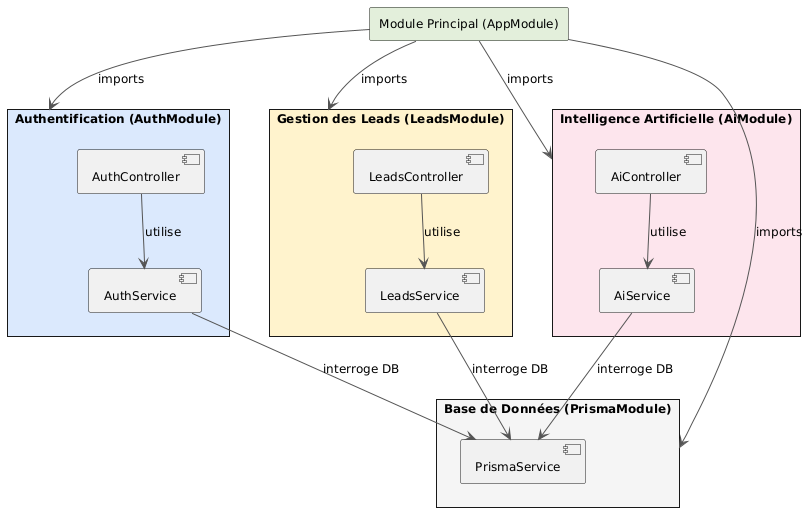
\includegraphics[width=\textwidth,height=0.82\textheight,keepaspectratio]{images/architecture_backend.png}
    \caption{Architecture modulaire du back-end NestJS}
    \label{fig:archi-backend}
\end{figure}

\subsubsection{Architecture Microservices -- Agent IA}

Le service de \textbf{Lead Scoring} est conçu comme un microservice indépendant basé sur \textbf{FastAPI} (Python). Ce service implémente un modèle de Machine Learning (\textit{Random Forest Classifier}) entraîné sur un dataset de scoring de leads. Il communique avec le backend NestJS via des appels HTTP REST.

L'architecture microservices intègre deux avantages majeurs :
\begin{itemize}
    \item \textbf{Indépendance technologique} : le service IA utilise Python et scikit-learn, tandis que le backend principal utilise Node.js/TypeScript, chaque service exploitant les meilleures technologies pour son domaine.
    \item \textbf{Scalabilité indépendante} : le service de scoring peut être mis à l'échelle indépendamment du backend principal en fonction de la charge de prédiction.
\end{itemize}

\begin{figure}[H]
    \centering
    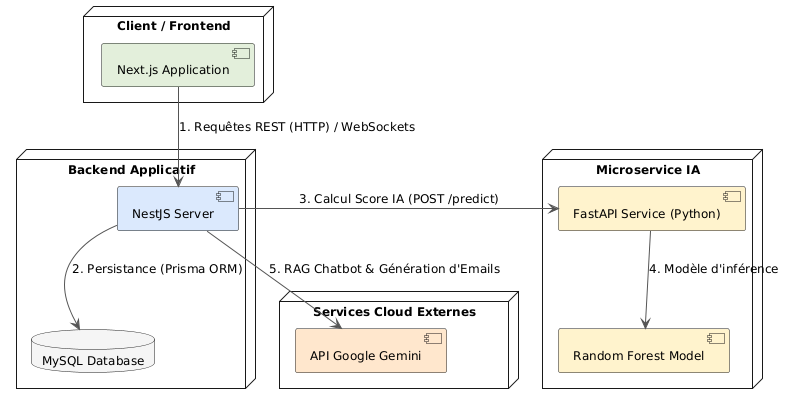
\includegraphics[width=\textwidth,height=0.82\textheight,keepaspectratio]{images/architecture_microservices.png}
    \caption{Architecture microservices -- Agent IA de scoring}
    \label{fig:archi-microservices}
\end{figure}

\subsubsection{Diagramme de composants back-end}

% \begin{figure}[H]
%     \centering
%     % \includegraphics[width=\textwidth]{images/diagramme_composants_backend.png}
%     \caption{Diagramme de composants back-end}
%     \label{fig:composants-backend}
% \end{figure}

%% ============================================================
%%  4.3  ENVIRONNEMENT DE DÉVELOPPEMENT
%% ============================================================
\section{Environnement de développement}

Dans cette partie, nous décrivons les différents outils matériels et logiciels utilisés tout au long de la concrétisation de notre solution.

\subsection{Technologies de programmation}

\subsubsection{Node.js}
Node.js est un environnement d'exécution JavaScript construit sur le moteur V8 de Google Chrome. Il dispose de fonctionnalités exceptionnelles qui en font un choix attrayant pour la création d'applications côté serveur, notamment des serveurs web et des services web. Node.js utilise un modèle d'entrées-sorties non bloquant, basé sur les événements, qui le rend léger et efficace, asynchrone par défaut. Dans notre projet, Node.js (version 22) constitue le socle d'exécution de notre backend NestJS et de notre frontend Next.js.
\begin{figure}[H]
    \centering
    
\includegraphics[width=0.6\textwidth,height=0.45\textheight,keepaspectratio]{images/node.png}
    \caption{Node.js}
    \label{fig:node}
\end{figure}

\subsubsection{Python}
Python est un langage de programmation interprété, polyvalent et à typage dynamique. Il est particulièrement prisé dans le domaine de la \textit{data science} et du \textit{machine learning} grâce à son écosystème riche en bibliothèques spécialisées. Dans notre projet, Python est utilisé pour le développement du microservice d'intelligence artificielle de scoring des leads, exploitant les bibliothèques \texttt{scikit-learn}, \texttt{pandas} et \texttt{numpy}.
\begin{figure}[H]
    \centering
    
\includegraphics[width=0.6\textwidth,height=0.45\textheight,keepaspectratio]{images/python.png}
    \caption{Python}
    \label{fig:python1}
\end{figure}

\subsection{Langages de programmation}

\subsubsection{TypeScript}
TypeScript est un langage compilé, fortement typé, orienté objet, conçu par Microsoft. Il représente un sur-ensemble typé de JavaScript, ajoutant le typage statique, les interfaces et les décorateurs. Dans notre projet, TypeScript est utilisé tant côté front-end (Next.js/React) que côté back-end (NestJS), garantissant une cohérence du code et une détection précoce des erreurs à la compilation.
\begin{figure}[H]
    \centering
    
\includegraphics[width=0.45\textwidth,height=0.4\textheight,keepaspectratio]{images/typescipt.png}
    \caption{TypeScript}
    \label{fig:typescript}
\end{figure}

\subsubsection{Python}
Python est utilisé comme langage principal pour le développement du microservice de Lead Scoring basé sur FastAPI. Sa syntaxe concise et ses bibliothèques de \textit{machine learning} (scikit-learn, pandas, numpy) en font le choix idéal pour l'implémentation de notre modèle prédictif \textit{Random Forest Classifier}.
\begin{figure}[H]
    \centering
    
\includegraphics[width=0.6\textwidth,height=0.45\textheight,keepaspectratio]{images/python.png}
    \caption{Python - Microservice IA}
    \label{fig:python2}
\end{figure}

\subsection{Frameworks}

\subsubsection{Next.js}
Next.js (version 16) est un framework React de production développé par Vercel. Il offre le rendu côté serveur (SSR), la génération de sites statiques (SSG), le routage basé sur le système de fichiers via l'App Router, ainsi qu'un système de middleware intégré. Dans notre projet, Next.js gère l'intégralité de l'interface utilisateur avec un système de routage basé sur les rôles (Admin et Sales Rep).
\begin{figure}[H]
    \centering
    
\includegraphics[width=0.6\textwidth,height=0.45\textheight,keepaspectratio]{images/next.png}
    \caption{Next.js}
    \label{fig:next}
\end{figure}

\subsubsection{NestJS}
NestJS (version 10) est un framework Node.js progressif pour la construction d'applications côté serveur efficaces et évolutives. Inspiré d'Angular, il adopte une architecture modulaire avec injection de dépendances, décorateurs et une structure opinionnée. Notre backend NestJS expose des API REST documentées via Swagger et gère l'authentification JWT, la communication WebSocket et l'envoi d'e-mails.
\begin{figure}[H]
    \centering
    
\includegraphics[width=0.6\textwidth,height=0.45\textheight,keepaspectratio]{images/nest.png}
    \caption{Nest.js}
    \label{fig:nest}
\end{figure}

\subsubsection{FastAPI}
FastAPI est un framework web Python moderne et haute performance pour la construction d'API. Il exploite les annotations de type Python pour la validation automatique des données et la génération de documentation OpenAPI. Dans notre projet, FastAPI héberge le modèle de \textit{machine learning} de scoring des leads et expose les endpoints de prédiction.
\begin{figure}[H]
    \centering
    
\includegraphics[width=0.6\textwidth,height=0.45\textheight,keepaspectratio]{images/fast.png}
    \caption{FastAPI}
    \label{fig:fastapi}
\end{figure}

\subsection{Base de données}

\subsubsection{Système de gestion de base de données}
\textbf{MySQL 8} : Tout au long du développement de notre application, nous avons utilisé MySQL 8 comme système de gestion de base de données relationnelle. MySQL offre une fiabilité, des performances et une facilité d'utilisation reconnues. Il gère l'ensemble des données de notre CRM : utilisateurs, leads, contacts, entreprises, pipelines, deals, tâches, tickets, e-mails, messages de chat et notifications.
\begin{figure}[H]
    \centering
    
\includegraphics[width=0.6\textwidth,height=0.45\textheight,keepaspectratio]{images/sql.png}
    \caption{MySQL}
    \label{fig:mysql}
\end{figure}

\subsubsection{ORM -- Prisma}
\textbf{Prisma} est un ORM (Object-Relational Mapping) moderne pour Node.js et TypeScript. Il fournit un client de base de données type-safe auto-généré, un système de migrations déclaratives et un langage de schéma intuitif. Prisma simplifie considérablement les interactions avec MySQL en offrant une API fluide et en garantissant la sécurité des types à la compilation.
\begin{figure}[H]
    \centering
    
\includegraphics[width=0.45\textwidth,height=0.4\textheight,keepaspectratio]{images/prisma.png}
    \caption{Prisma}
    \label{fig:prisma}
\end{figure}

\subsection{Outils de développement}

\subsubsection{Visual Studio Code}
Visual Studio Code (VS Code) est un éditeur de code source léger mais puissant, développé par Microsoft. Il supporte le débogage, le contrôle Git intégré, la coloration syntaxique, l'auto-complétion intelligente et un écosystème riche en extensions. VS Code est notre IDE principal pour le développement TypeScript (front-end et back-end) et Python (agent IA).
\begin{figure}[H]
    \centering
    
\includegraphics[width=0.45\textwidth,height=0.4\textheight,keepaspectratio]{images/vscode.png}
    \caption{Visual Studio Code}
    \label{fig:vscode}
\end{figure}

\subsubsection{Docker \& Docker Compose}
Docker est une plateforme de conteneurisation permettant de placer nos applications ainsi que leurs dépendances dans des conteneurs indépendants et réutilisables. Docker Compose gère l'ensemble de ces quatre services (MySQL, Backend NestJS, Frontend Next.js, AI Agent FastAPI) avec un fichier de configuration \texttt{docker-compose.yaml}.
\begin{figure}[H]
    \centering
    
\includegraphics[width=0.6\textwidth,height=0.45\textheight,keepaspectratio]{images/docker.png}
    \caption{Docker}
    \label{fig:docker}
\end{figure}

\subsubsection{Kubernetes \& Helm}
Kubernetes est une plate-forme open source d'orchestration de containers qui facilite le déploiement, le scaling et la gestion des applications dans des conteneurs. Helm, qui est un package manager pour Kubernetes, nous donne la possibilité de créer des charts réutilisables pour chaque service de notre plate-forme.
\begin{figure}[H]
    \centering
    
\includegraphics[width=0.6\textwidth,height=0.45\textheight,keepaspectratio]{images/kubernetes.png}
    \caption{Kubernetes and Helm}
    \label{fig:kubernetes}
\end{figure}

\subsubsection{GitHub \& GitHub Actions}
Nous utilisons GitHub comme plateforme pour héberger nos codes sources. GitHub Actions fournit un pipeline CI/CD pour nous avec quatre jobs : build/test des applications, la vérification de la qualité du code par ESLint, la construction de l'image Docker puis sa publication dans Docker Hub, et enfin la modification du tag image des charts Helm.
\begin{figure}[H]
    \centering
    
\includegraphics[width=0.6\textwidth,height=0.45\textheight,keepaspectratio]{images/github.png}
    \caption{GitHub and GitHub Actions}
    \label{fig:github}
\end{figure}

\subsubsection{Postman}
Postman est un outil de test excellent pour l'examen et le test de nos API RESTful. Postman nous offre une interface utilisateur où l'on peut faire nos requêtes HTTP sans avoir besoin de coder pour tester la bonne marche de nos endpoints NestJS et FastAPI.
\begin{figure}[H]
    \centering
    
\includegraphics[width=0.6\textwidth,height=0.45\textheight,keepaspectratio]{images/postman.png}
    \caption{Postman}
    \label{fig:postman}
\end{figure}

\subsubsection{Swagger}
Swagger (à travers le module \texttt{@nestjs/swagger}) fournit une documentation de notre API REST backend en temps réel avec un interface interactif. Cette documentation est accessible depuis le navigateur et elle aide les développeurs à explorer tous les endpoints.
\begin{figure}[H]
    \centering
    
\includegraphics[width=0.45\textwidth,height=0.4\textheight,keepaspectratio]{images/swagger.png}
    \caption{Swagger}
    \label{fig:swagger}
\end{figure}

\subsubsection{Power BI}
Le Power BI est un outil d'analyse d'affaires ou Business Intelligence développé par Microsoft qui est utilisé pour l'analyse interactive via la conception de tableaux de bord. Pour le projet courant, le Power BI est configuré afin d'accéder à notre base de données MySQL et générer des rapports interactifs des données sur nos performances et nos leads.
\begin{figure}[H]
    \centering
    
\includegraphics[width=0.6\textwidth,height=0.45\textheight,keepaspectratio]{images/powerbi.png}
    \caption{Microsoft Power BI}
    \label{fig:powerbi}
\end{figure}

\subsubsection{Draw.io}
Draw.io est un logiciel d'édition de diagramme en ligne totalement gratuit pour créer différents types de diagramme comme le diagramme UML, les diagrammes de séquence, les diagrammes de déploiement et des modèles. Nous avons utilisé Draw.io pour concevoir toutes les figures mentionnées dans ce rapport.
\begin{figure}[H]
    \centering
    
\includegraphics[width=0.6\textwidth,height=0.45\textheight,keepaspectratio]{images/draw.png}
    \caption{Draw.io}
    \label{fig:drawio}
\end{figure}

\subsubsection{Overleaf}
Overleaf est un site collaboratif d'écriture basé sur le logiciel de traitement de texte LaTeX. Il permet à plusieurs personnes de travailler simultanément sur un même document et propose de nombreux modèles de documents déjà prédéfinis. Nous avons utilisé Overleaf pour rédiger ce rapport de PFE.
\begin{figure}[H]
    \centering
    
\includegraphics[width=0.6\textwidth,height=0.45\textheight,keepaspectratio]{images/overleaf.png}
    \caption{Overleaf}
    \label{fig:overleaf}
\end{figure}

%% ============================================================
%%  4.4  PRÉSENTATION DE L'APPLICATION
%% ============================================================
\section{Présentation de l'application}

Dans cette partie, nous donnerons un aperçu des interfaces de notre plateforme CRM développées à travers quelques captures d'écran.

\subsection{Module d'authentification}

\subsubsection{Interface de connexion}
Le module de connexion autorise les utilisateurs à se connecter en utilisant leurs adresses électroniques et mots de passe. La validation des informations est effectuée par JWT (JSON Web Token) et ensuite, ils sont réorientés au tableau de bord qui leur est dédié d'après leur statut qui peut être soit \textbf{Admin} soit \textbf{Rep}.

\begin{figure}[H]
    \centering
    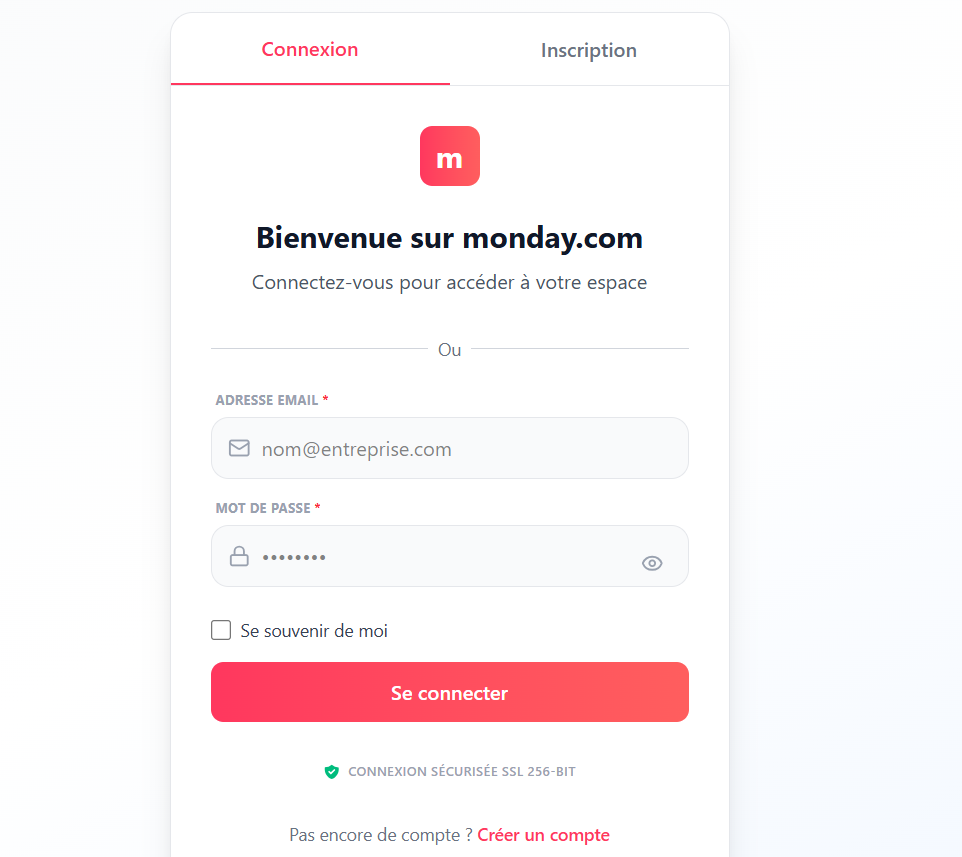
\includegraphics[width=\textwidth,height=0.82\textheight,keepaspectratio]{images/interface_login.png}
    \caption{Interface de connexion}
    \label{fig:login}
\end{figure}

\subsubsection{Interface d'inscription}
The registration interface provides an opportunity for a new user to register by entering his name, email address, password, and company. The role defaults to Sales Representative (Rep).

\begin{figure}[H]
    \centering
    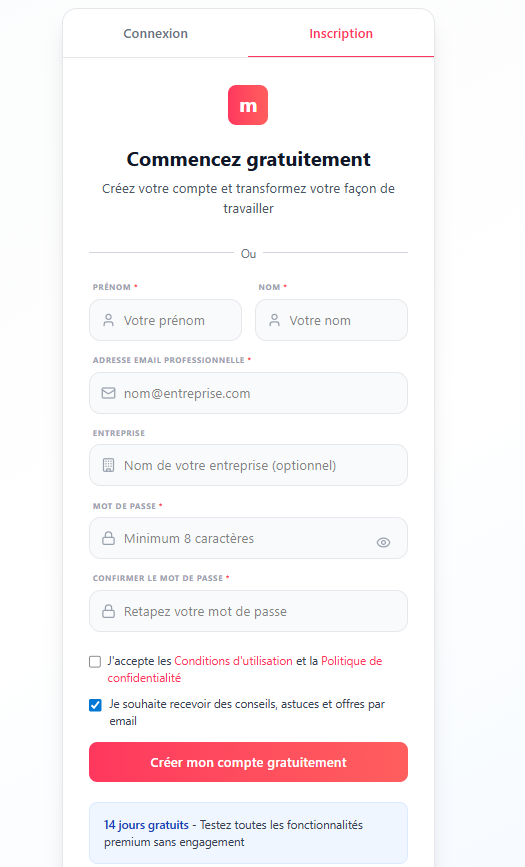
\includegraphics[width=\textwidth,height=0.82\textheight,keepaspectratio]{images/interface_register.png}
    \caption{Interface d'inscription}
    \label{fig:register}
\end{figure}

\subsection{Partie Admin (Sales Manager)}

\subsubsection{Interface tableau de bord Admin}
Après l'authentification, le Sales Manager est automatiquement dirigé vers son dashboard principal. Ce dashboard fournit un aperçu des principaux KPIs qui incluent le nombre total de leads, de contacts, de deals actuels, de taux de conversion, ainsi qu'un diagramme pour analyser l'évolution du chiffre d'affaires et la segmentation des leads selon leurs statuts.

\begin{figure}[H]
    \centering
    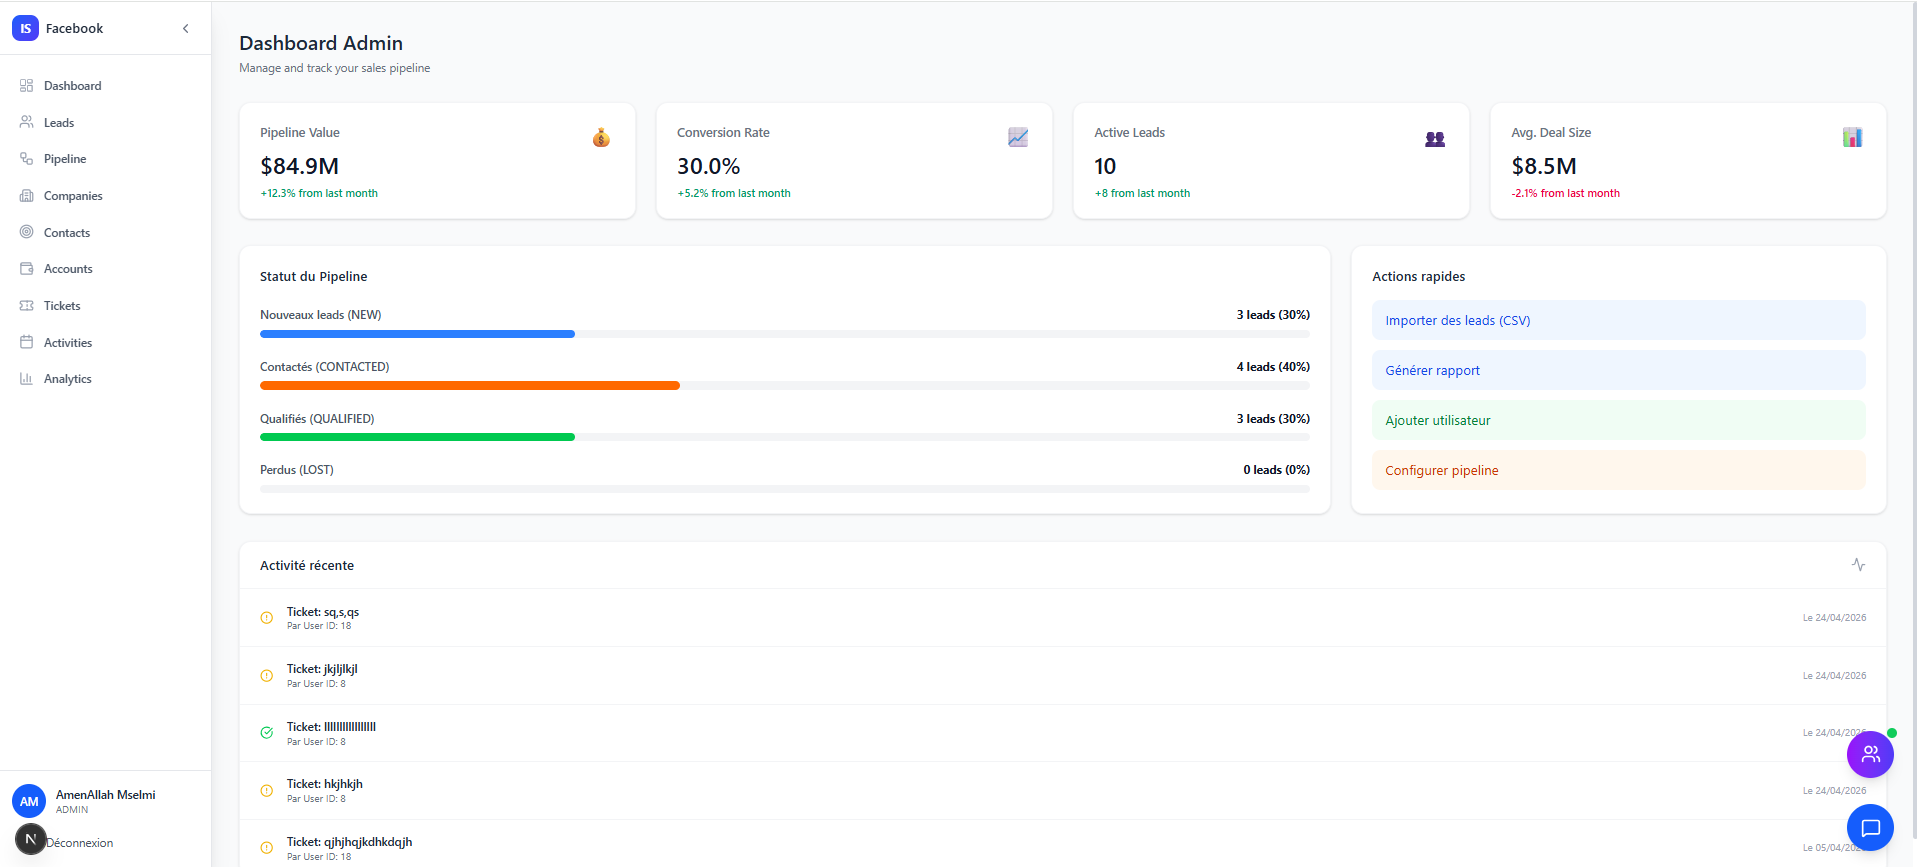
\includegraphics[width=\textwidth,height=0.82\textheight,keepaspectratio]{images/interface_dashboard_admin.png}
    \caption{Interface tableau de bord Admin}
    \label{fig:dashboard-admin}
\end{figure}

\subsubsection{Interface gestion des leads}
Cette interface aide l'administrateur à voir, rechercher, filtrer et gérer tous les leads. Les informations affichées pour chaque lead incluent son nom, email, numéro de téléphone, statut (Nouveau, Contacté, Qualifié, Perdu), valeur du lead et le score de l'IA. En outre, l'administrateur peut accéder aux informations détaillées sur un lead, y compris ses notes, tâches, tickets et activités.

\begin{figure}[H]
    \centering
    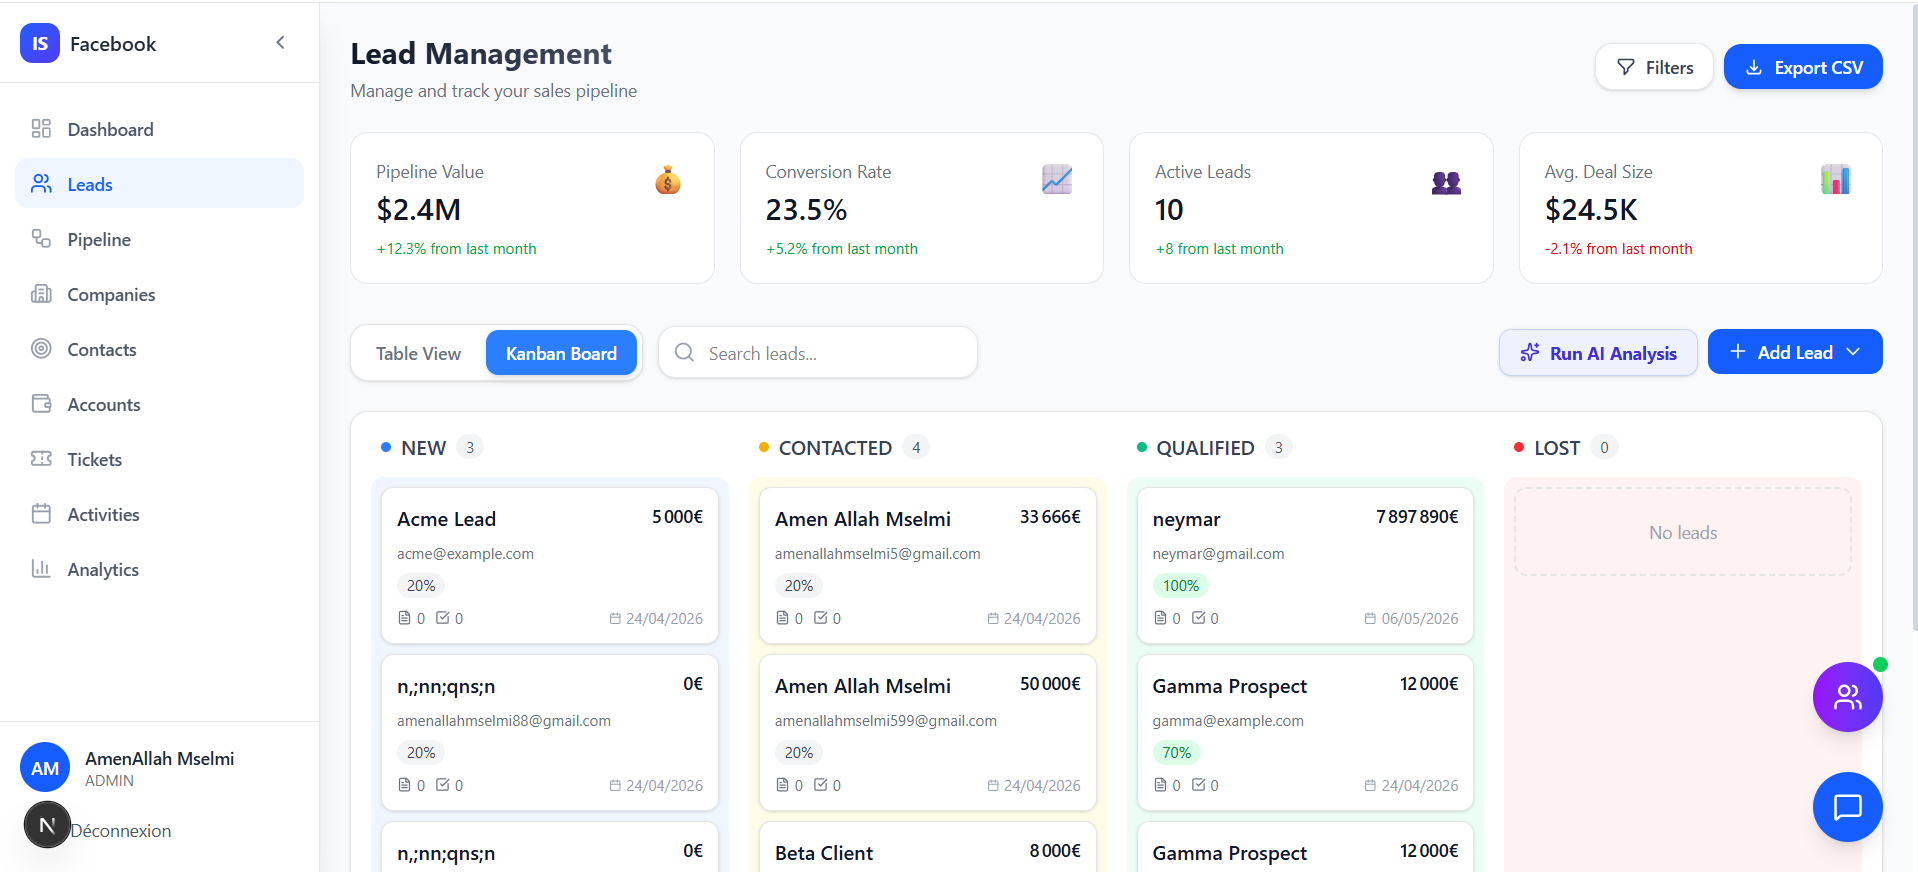
\includegraphics[width=\textwidth,height=0.82\textheight,keepaspectratio]{images/interface_leads.png}
    \caption{Interface gestion des leads}
    \label{fig:leads}
\end{figure}

\subsubsection{Interface détails d'un lead avec scoring IA}
Le score de conversion, qui est calculé par le modèle d'intelligence artificielle (Random Forest), est également visible lorsqu'un administrateur accède à des informations sur un lead. Les informations présentées comprennent la probabilité de conversion, la chaleur du lead (chaud, tiède, froid), ainsi que les principales raisons derrière son score.

\begin{figure}[H]
    \centering
    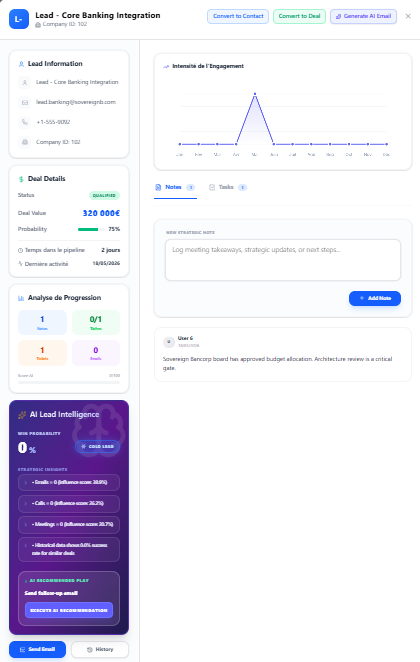
\includegraphics[width=\textwidth,height=0.82\textheight,keepaspectratio]{images/interface_lead_scoring.png}
    \caption{Interface détails d'un lead avec scoring IA}
    \label{fig:lead-scoring}
\end{figure}

\subsubsection{Interface gestion des contacts}
Cette interface liste tous les contacts disponibles dans le CRM. On peut effectuer une recherche, un filtre sur le statut (Active/Inactive), et voir toutes les informations de contact, à savoir leur entreprise correspondante, les courriels et tickets associés.

\begin{figure}[H]
    \centering
    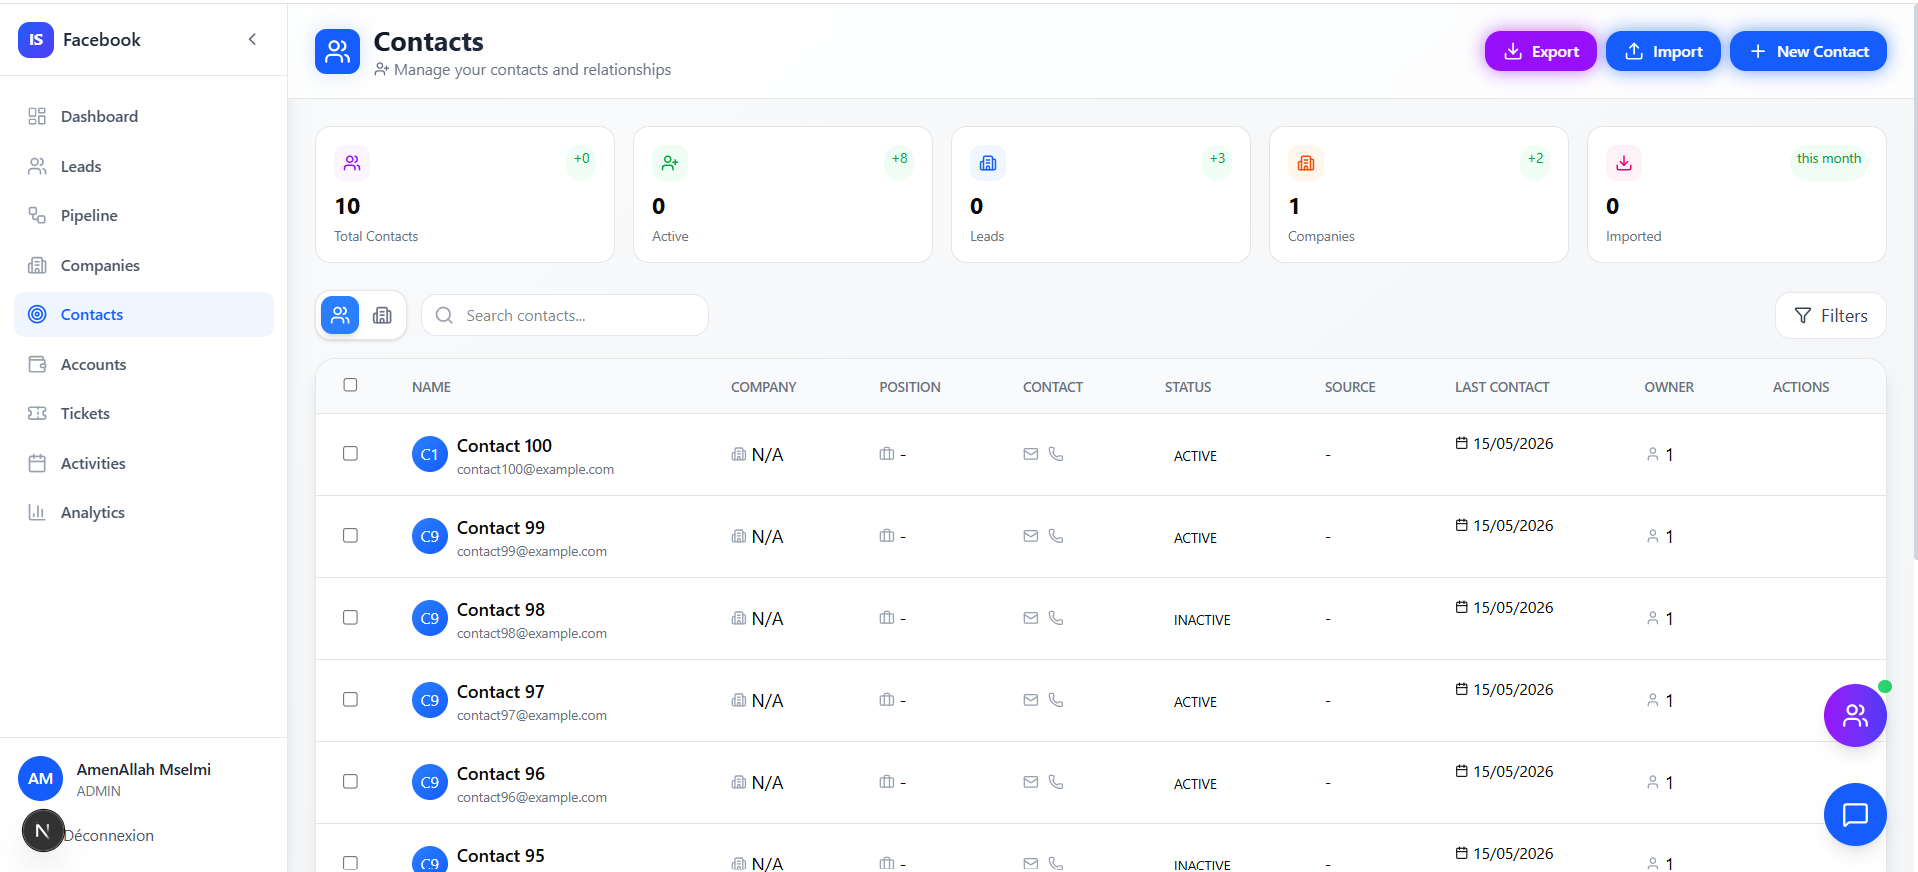
\includegraphics[width=\textwidth,height=0.82\textheight,keepaspectratio]{images/interface_contacts.png}
    \caption{Interface gestion des contacts}
    \label{fig:contacts}
\end{figure}

\subsubsection{Interface gestion des entreprises}
The interface for managing companies shows all the customer companies. Each company is displayed with its name, business sector (Technology, Finance, Healthcare, Education), size (Small, Medium, Large), location, and turnover.

\begin{figure}[H]
    \centering
    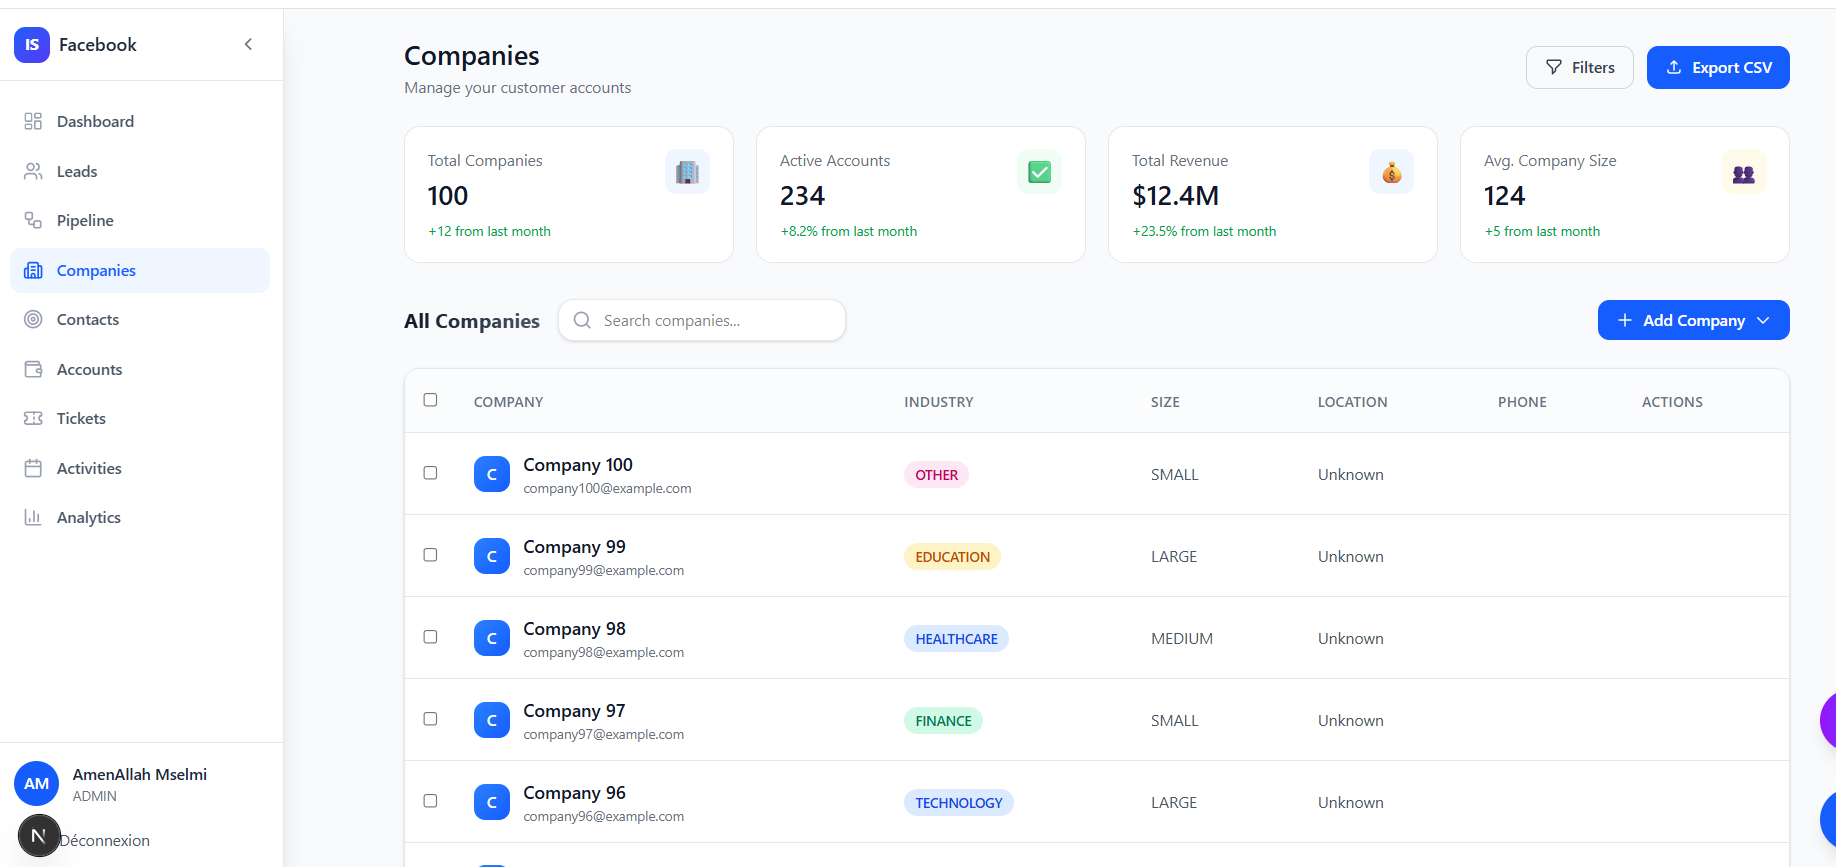
\includegraphics[width=\textwidth,height=0.82\textheight,keepaspectratio]{images/interface_companies.png}
    \caption{Interface gestion des entreprises}
    \label{fig:companies}
\end{figure}

\subsubsection{Interface Pipeline de vente}
La fenêtre de l'interface de pipeline de vente est constituée d'une représentation Kanban de l'affaire qui se divise en plusieurs étapes, notamment Nouvelle, Contactée, Qualifiée, Proposée, Négociée, Gagnée ou Perdue. L'admin peut voir les informations de toutes les affaires dans lesquelles se trouve la société, comme leur valeur, probabilité et date estimée de clôture.

\begin{figure}[H]
    \centering
    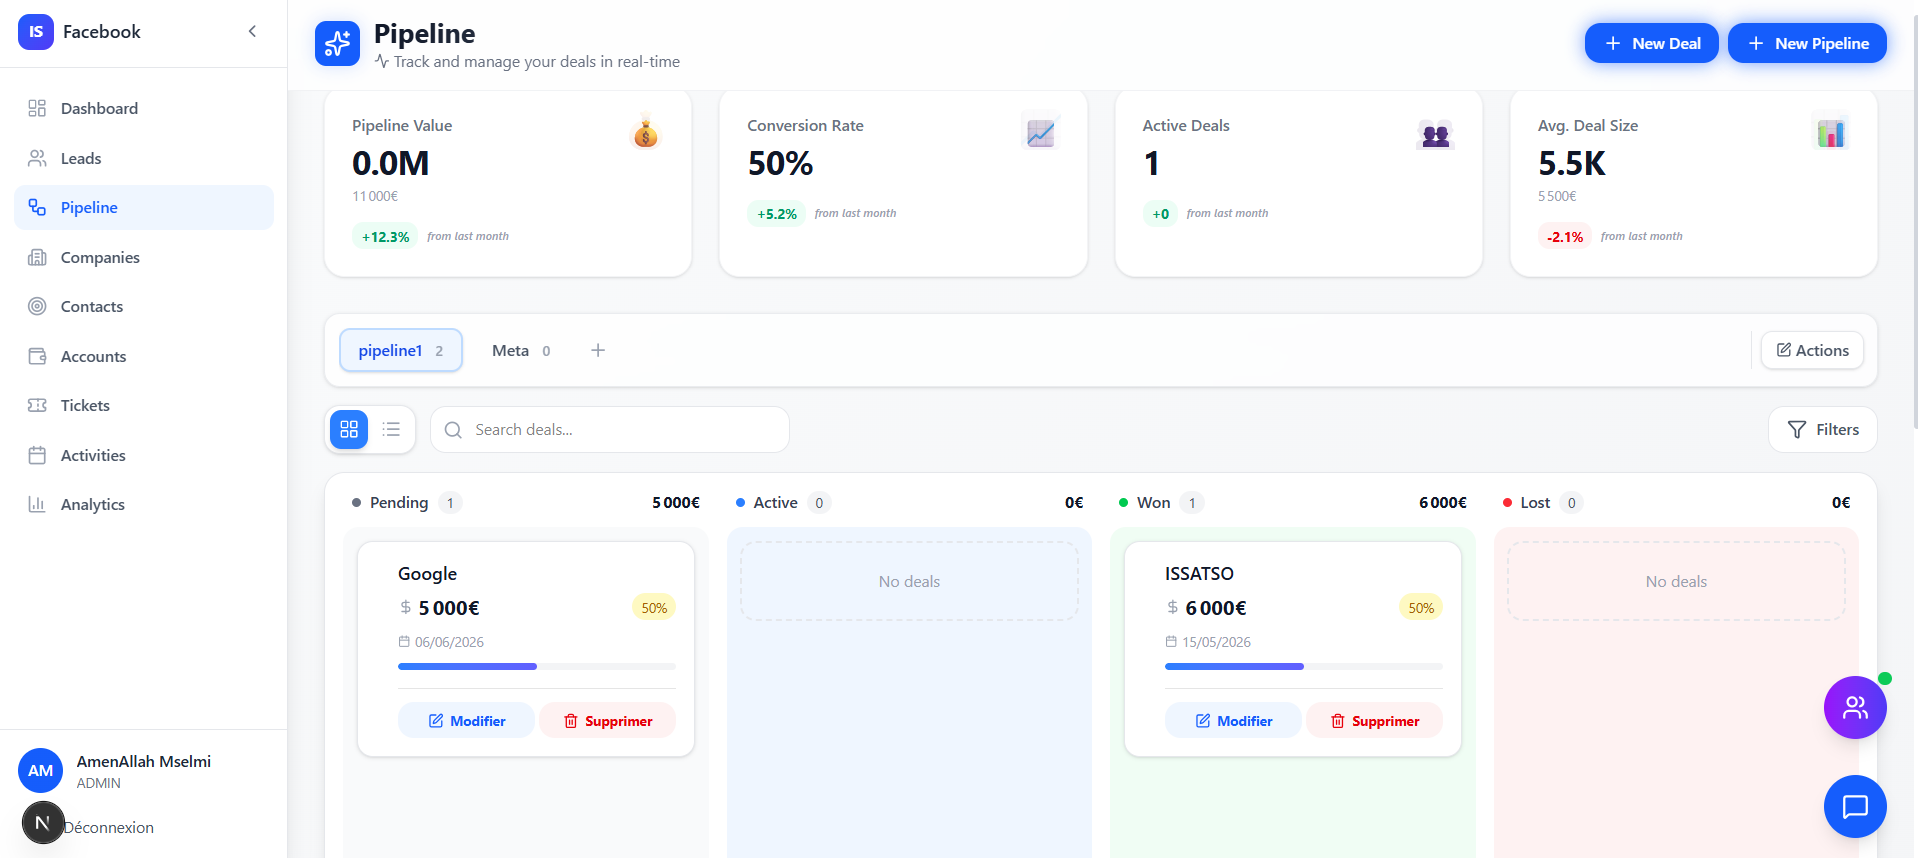
\includegraphics[width=\textwidth,height=0.82\textheight,keepaspectratio]{images/interface_pipeline.png}
    \caption{Interface Pipeline de vente}
    \label{fig:pipeline}
\end{figure}

\subsubsection{Interface gestion des tickets}
La gestion des billets sert à gérer la demande de soutien. La description du billet comprend le nom, la description, l'état (Nouveau, Ouvert, Attendu, Résolu, Fermé) ainsi que la priorité (Basse, Moyenne, Élevée, Critique).

\begin{figure}[H]
    \centering
    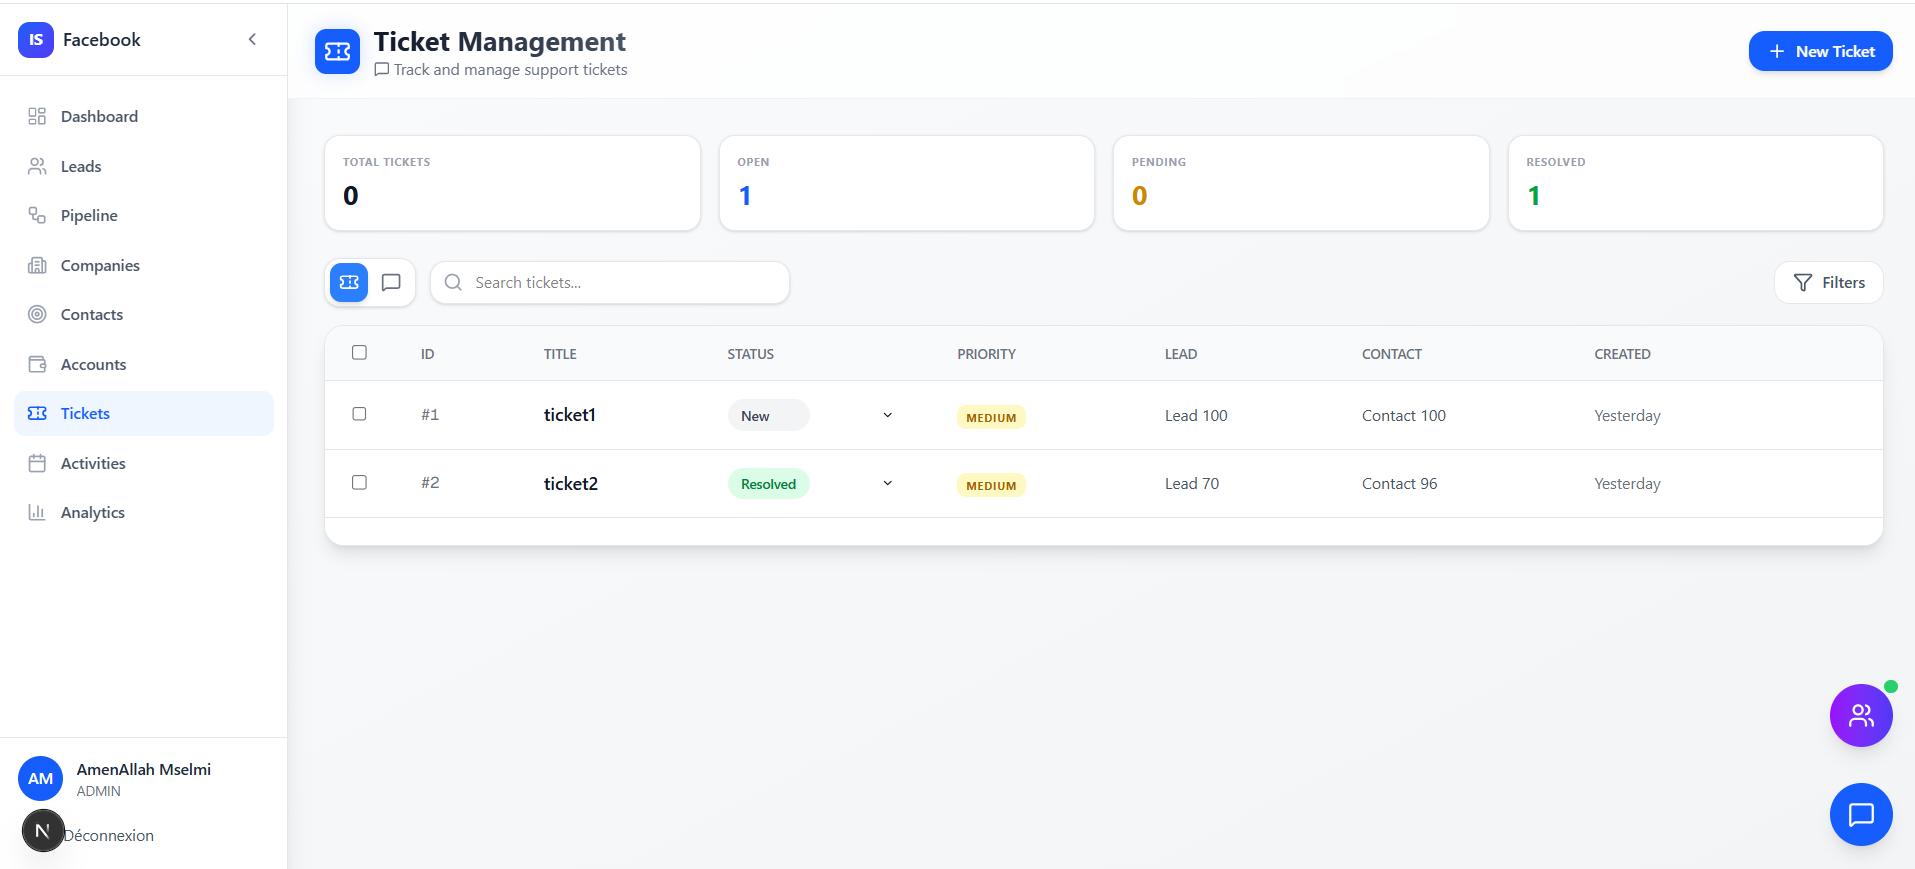
\includegraphics[width=\textwidth,height=0.82\textheight,keepaspectratio]{images/interface_tickets.png}
    \caption{Interface gestion des tickets}
    \label{fig:tickets}
\end{figure}

\subsubsection{Interface Analytics}
Le logiciel analytique permet des visualisations complexes basées sur les données issues du CRM : graphiques de performance de vente, distribution des leads selon l'origine, évolutions temporelles des taux de conversion et productivité des ventes.

\begin{figure}[H]
    \centering
    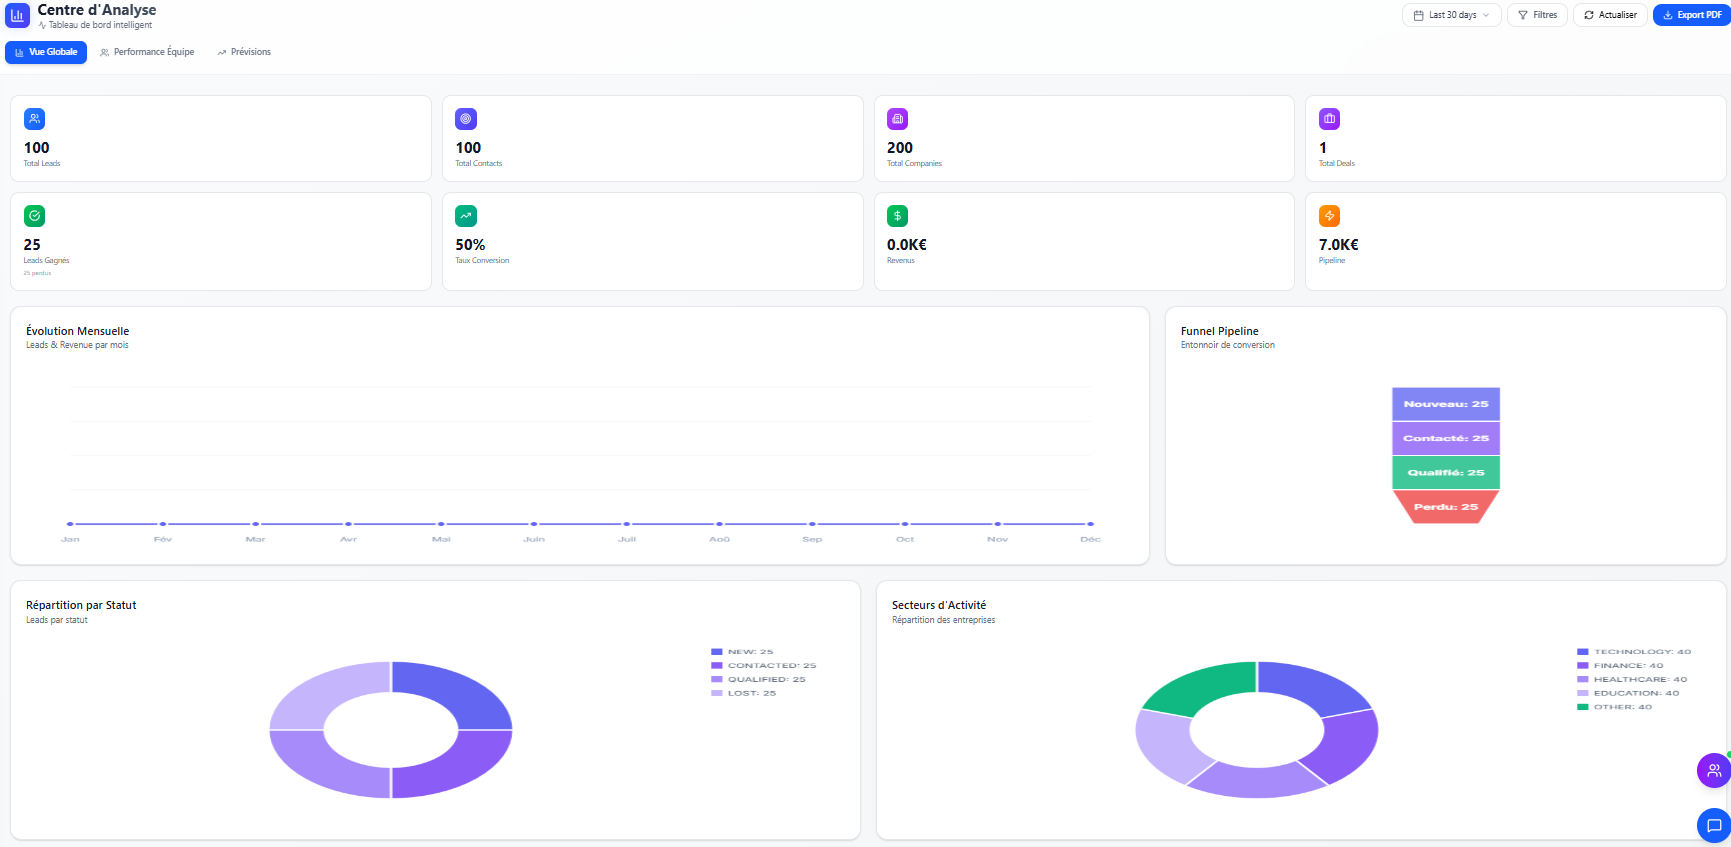
\includegraphics[width=\textwidth,height=0.82\textheight,keepaspectratio]{images/interface_analytics1.png}
    \caption{Interface Analytics - Vue d'ensemble}
    \label{fig:analytics1}
\end{figure}

\begin{figure}[H]
    \centering
    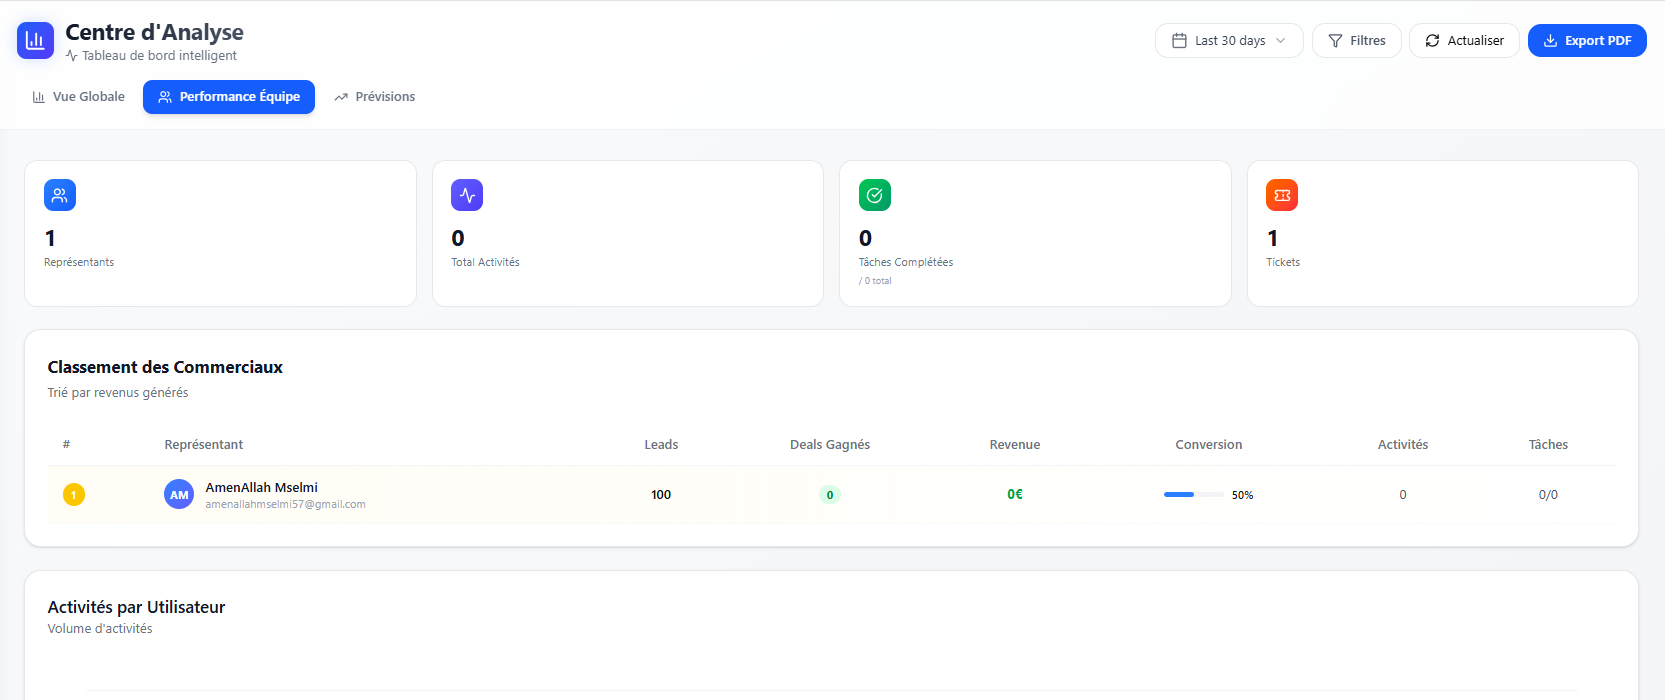
\includegraphics[width=\textwidth,height=0.82\textheight,keepaspectratio]{images/interface_analytics2.png}
    \caption{Interface Analytics - Performance d'équipe}
    \label{fig:analytics2}
\end{figure}

\begin{figure}[H]
    \centering
    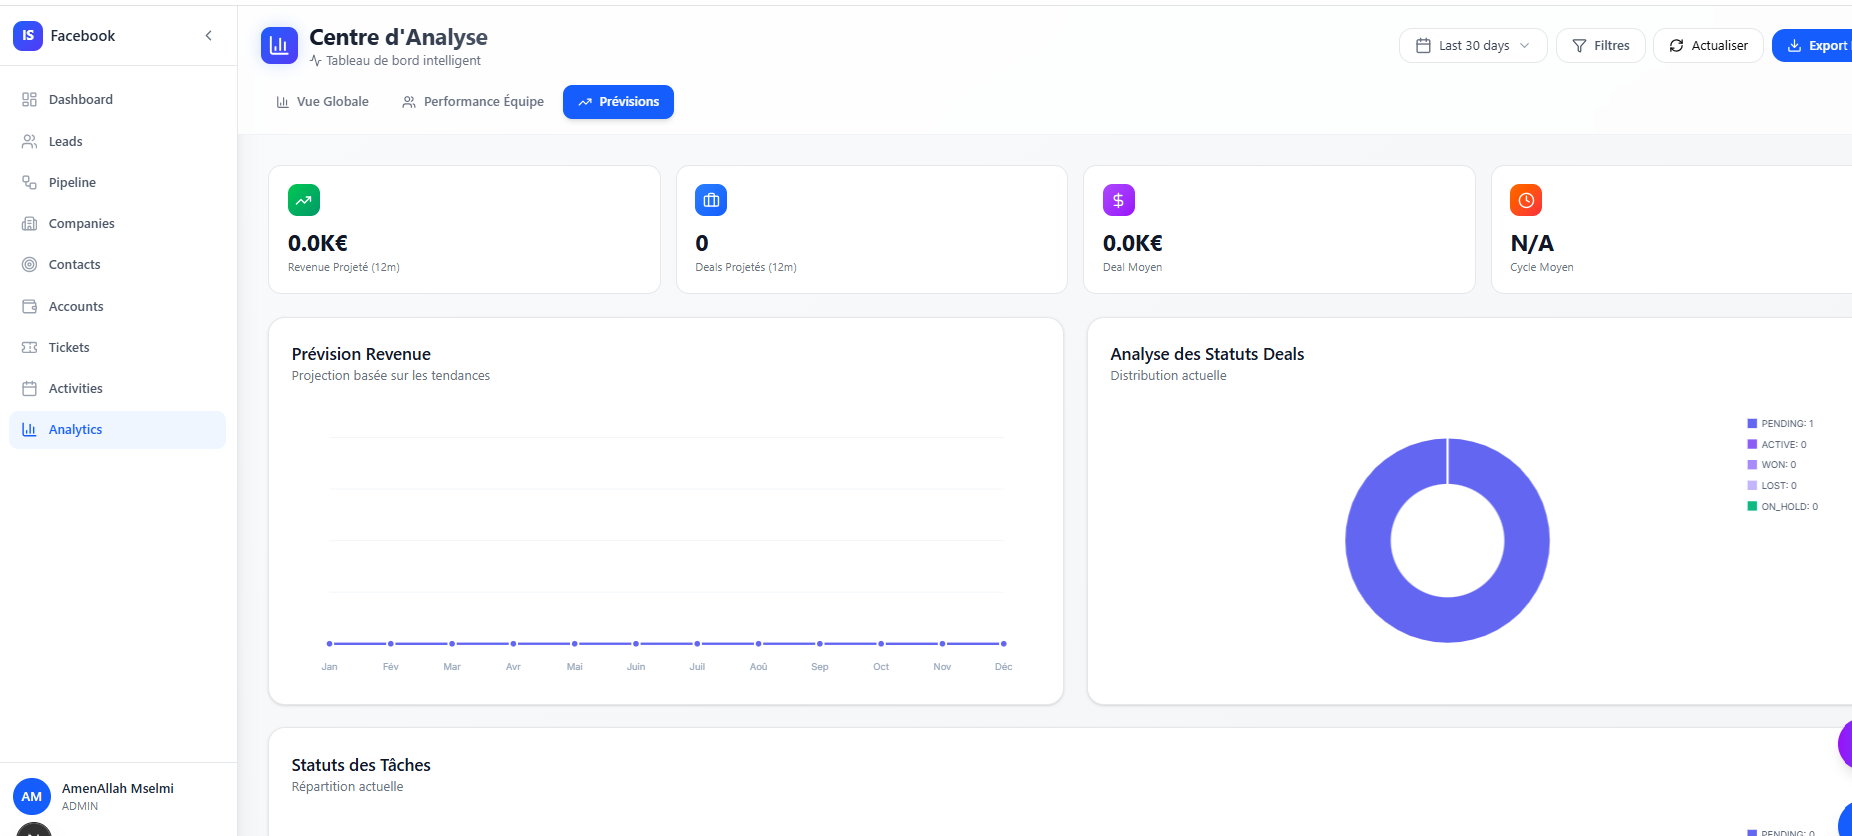
\includegraphics[width=\textwidth,height=0.82\textheight,keepaspectratio]{images/interface_analytics3.png}
    \caption{Interface Analytics - Prévisions}
    \label{fig:analytics3}
\end{figure}

\subsubsection{Interface gestion des comptes}
Il y a une interface pour la gestion des comptes où l'administrateur peut ajouter des comptes aux Sales Reps, modifier les paramètres de ces comptes, et activer ou désactiver ces comptes.

\begin{figure}[H]
    \centering
    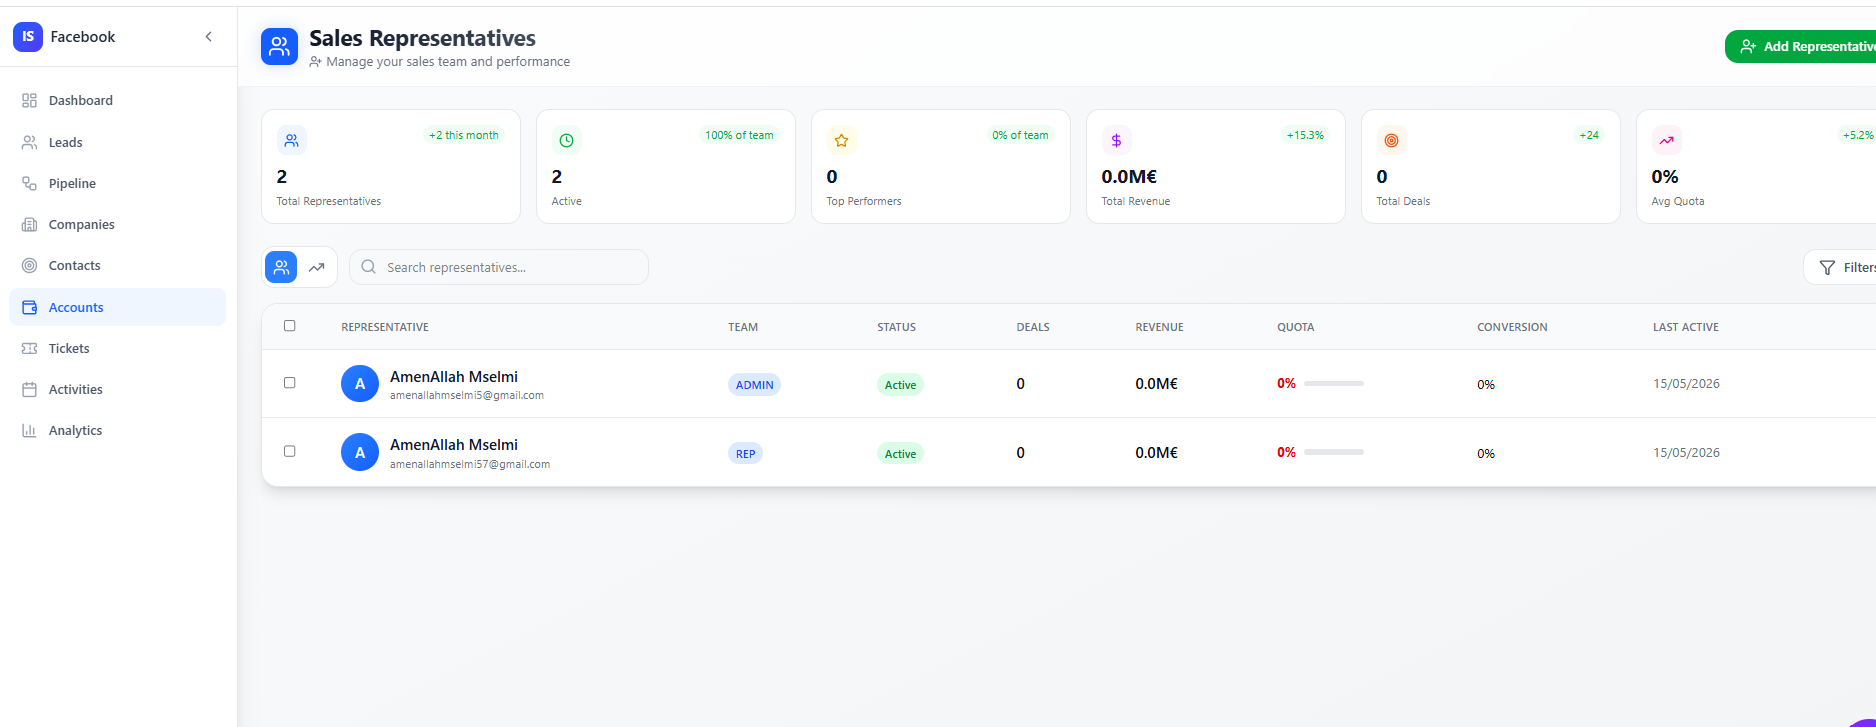
\includegraphics[width=\textwidth,height=0.82\textheight,keepaspectratio]{images/interface_accounts.png}
    \caption{Interface gestion des comptes utilisateurs}
    \label{fig:accounts}
\end{figure}

\subsection{Partie Sales Representative (Rep)}

\subsubsection{Interface tableau de bord Rep}
Dashboard du Sales Representative indique ses propres KPIs : lead assignés, deals actifs, les tâches qui lui sont attribuées et des tickets qu'il possède. Le design donne une vue d'ensemble de son travail commercial quotidien.

\begin{figure}[H]
    \centering
    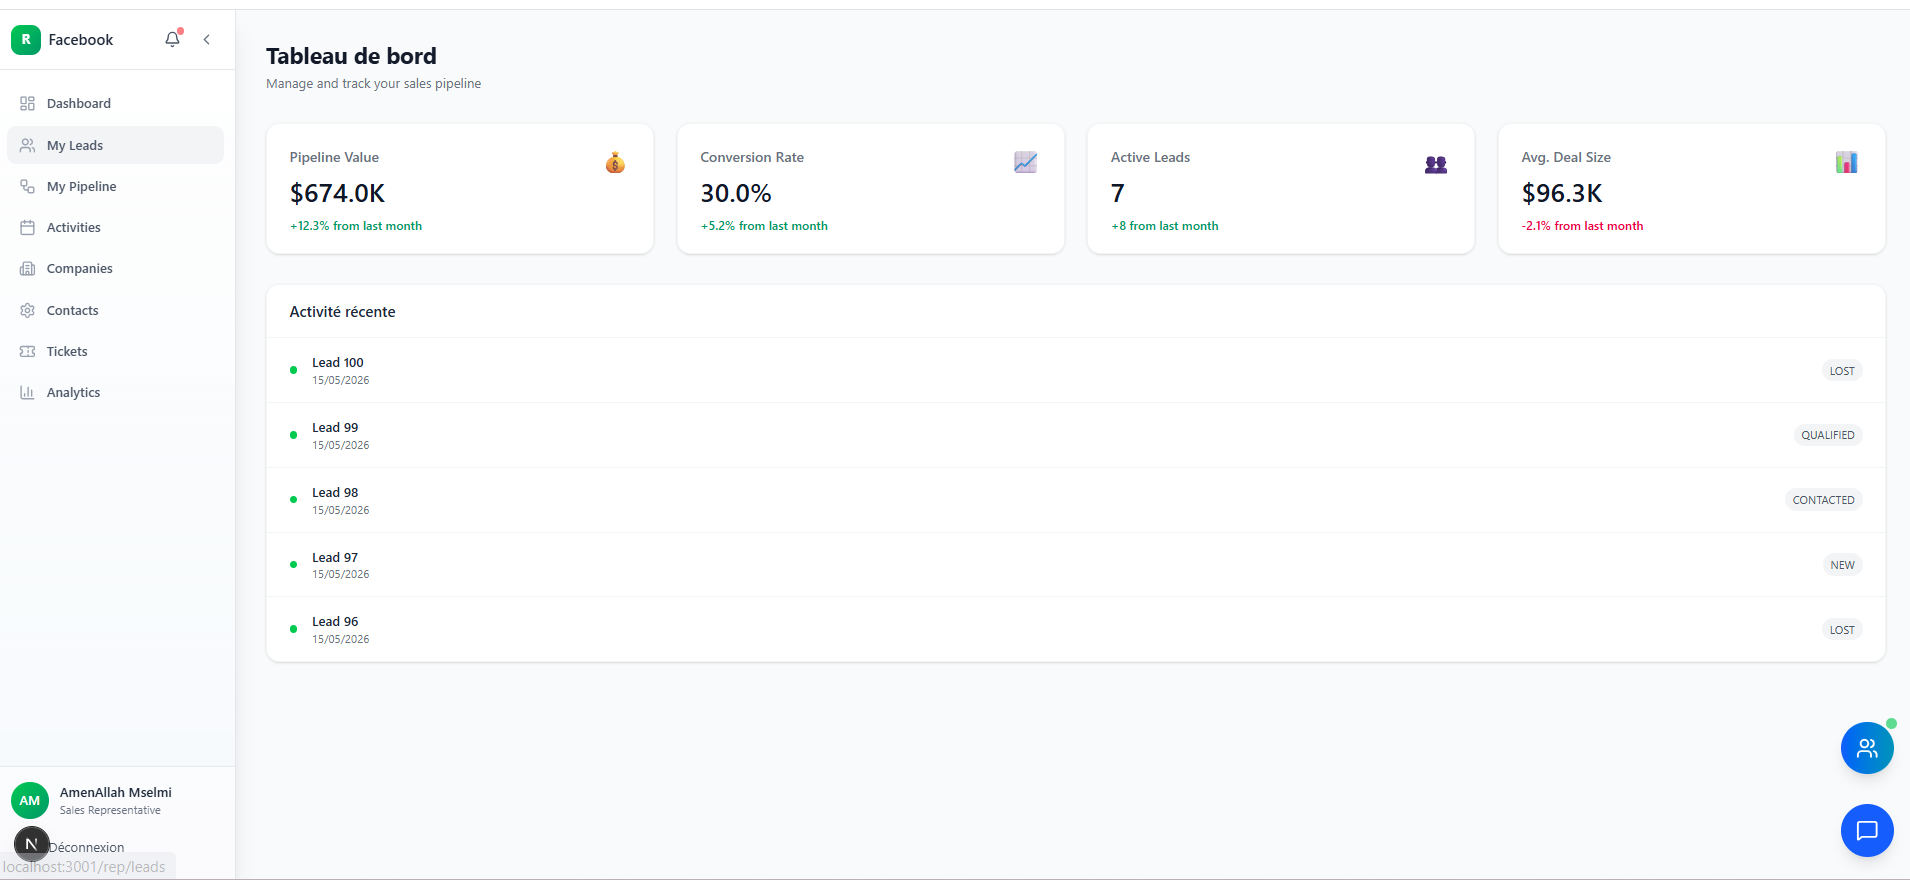
\includegraphics[width=\textwidth,height=0.82\textheight,keepaspectratio]{images/interface_dashboard_rep.png}
    \caption{Interface tableau de bord Sales Representative}
    \label{fig:dashboard-rep}
\end{figure}

\subsubsection{Interfaces du Rep -- Leads, Contacts et Pipeline}
Le Sales Representative a des interfaces qui sont comparables à celles de l'Admin mais uniquement sur ses propres données. Il peut gérer ses leads, contacts et pipeline personnels, en ayant la capacité d'ajouter des commentaires, créer des tâches et envoyer des messages électroniques.

\begin{figure}[H]
    \centering
    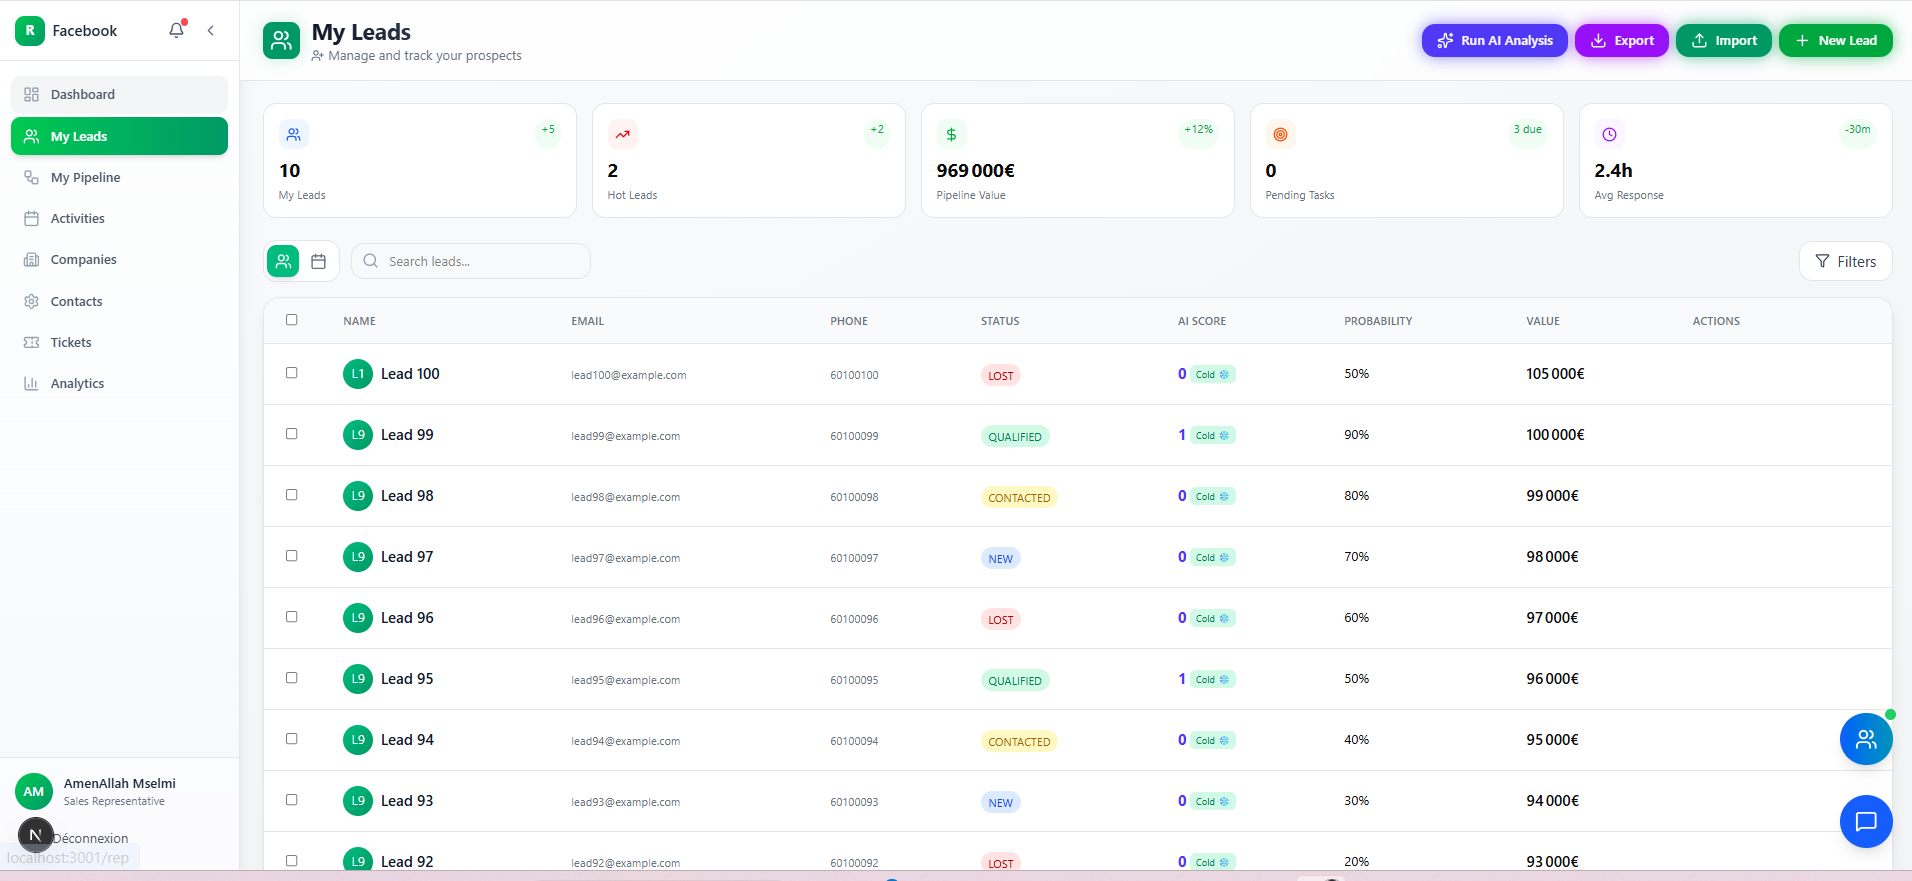
\includegraphics[width=\textwidth,height=0.82\textheight,keepaspectratio]{images/interface_rep_leads.png}
    \caption{Interface leads du Sales Representative}
    \label{fig:rep-leads}
\end{figure}

\subsection{Fonctionnalités transversales}

\subsubsection{Interface de Chat en temps réel}
Le module de chat est constitué d'une interface qui facilite la communication en temps réel entre les utilisateurs via WebSocket (Socket.io). Il permet aux utilisateurs d'échanger des messages, d'avoir des conversations privées ou de groupe, et d'être notifiés lorsqu'ils reçoivent un nouveau message.

\begin{figure}[H]
    \centering
    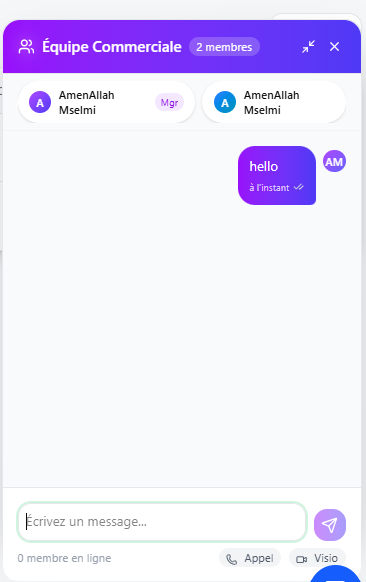
\includegraphics[width=\textwidth,height=0.82\textheight,keepaspectratio]{images/interface_chat.png}
    \caption{Interface de Chat en temps réel}
    \label{fig:chat}
\end{figure}

\subsubsection{Interface d'import CSV}
L'assistant d'import des données CSV donne un assistant étape par étape, permettant la facilité d'importer de nombreuses données de leads ou de contacts d'un fichier CSV. Les utilisateurs peuvent mapper les colonnes du fichier avec les champs CRM et importer les données.

\begin{figure}[H]
    \centering
    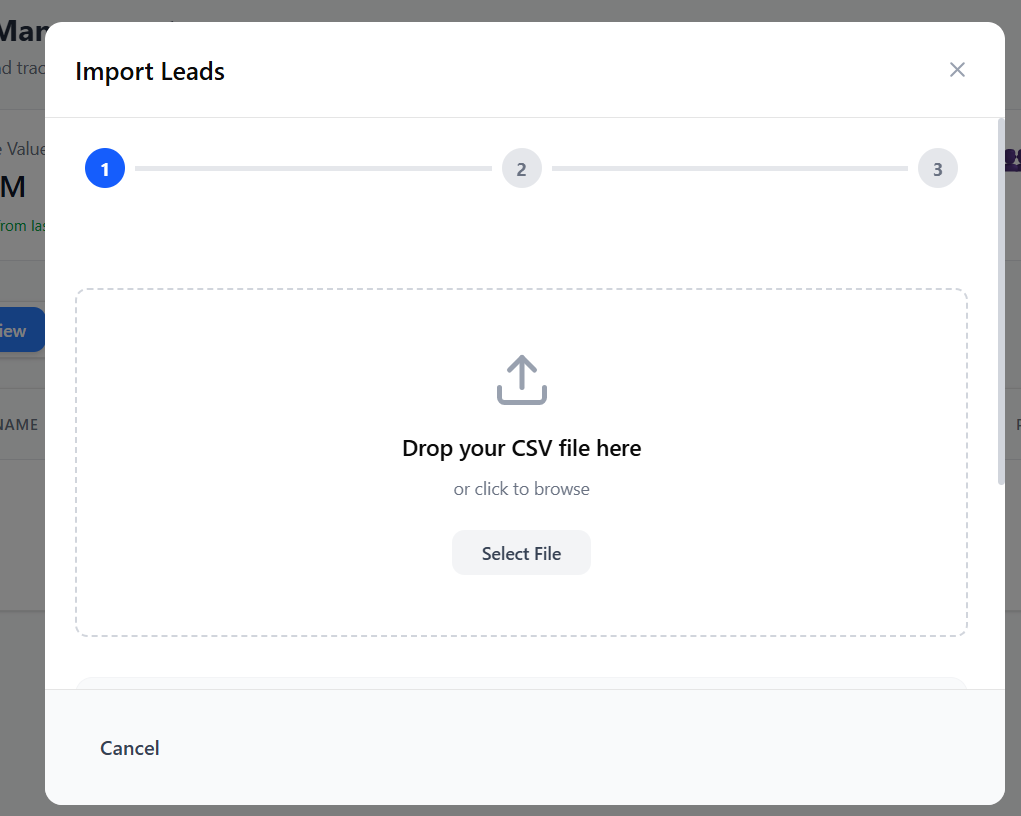
\includegraphics[width=\textwidth,height=0.82\textheight,keepaspectratio]{images/interface_csv_import1.png}
    \caption{Interface d'import CSV - Étape 1}
    \label{fig:csv-import1}
\end{figure}

\begin{figure}[H]
    \centering
    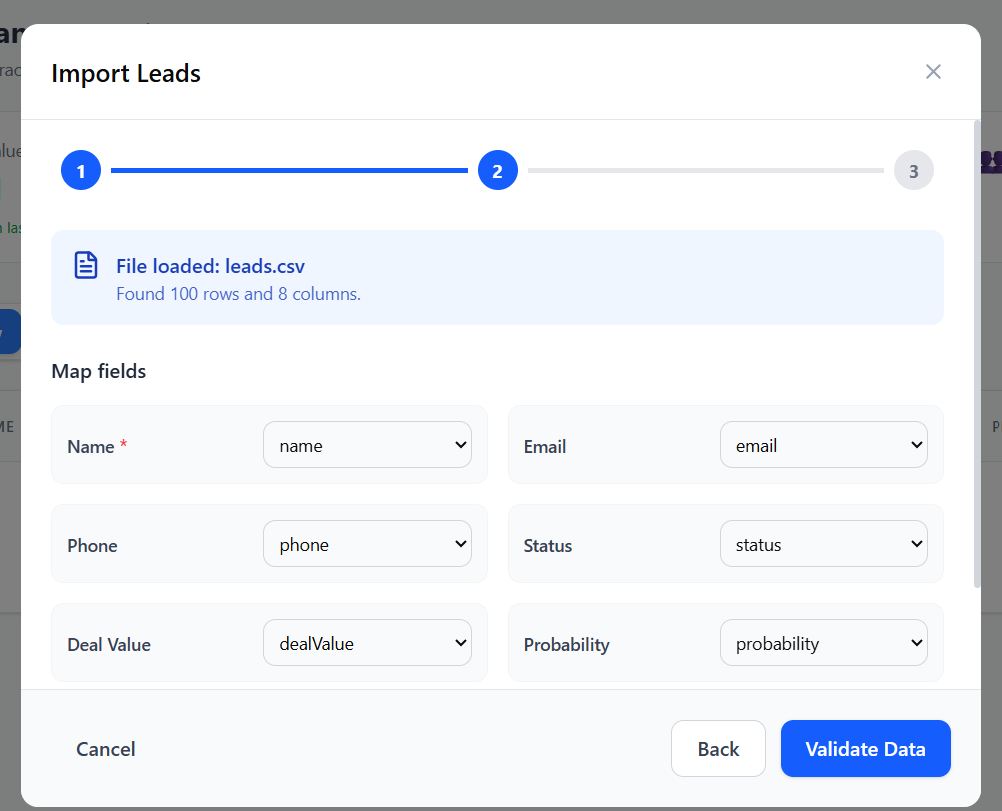
\includegraphics[width=\textwidth,height=0.82\textheight,keepaspectratio]{images/interface_csv_import2.png}
    \caption{Interface d'import CSV - Étape 2}
    \label{fig:csv-import2}
\end{figure}

\begin{figure}[H]
    \centering
    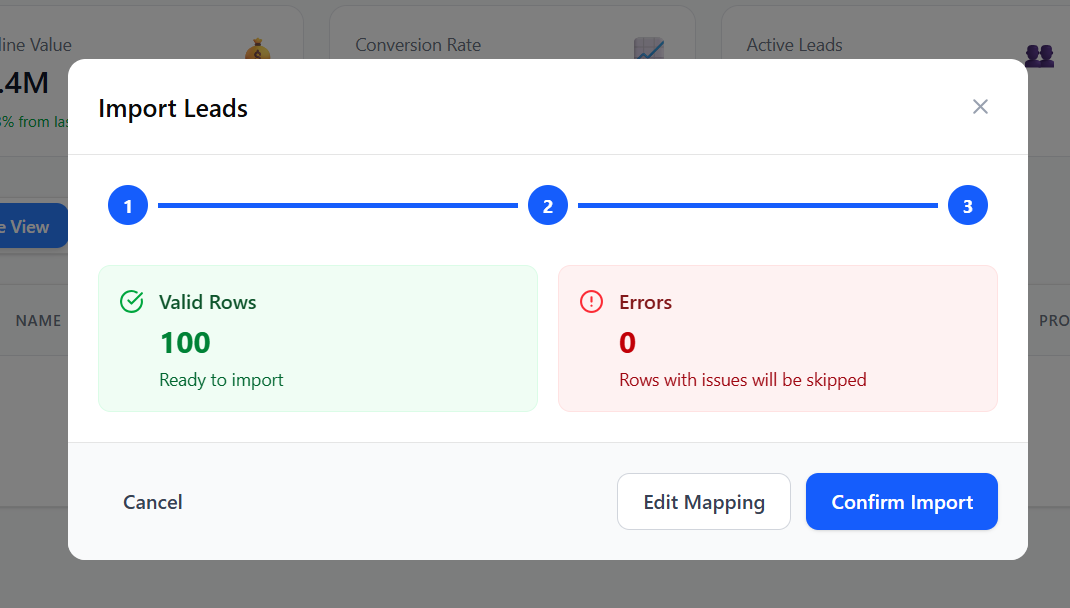
\includegraphics[width=\textwidth,height=0.82\textheight,keepaspectratio]{images/interface_csv_import3.png}
    \caption{Interface d'import CSV - Étape 3}
    \label{fig:csv-import3}
\end{figure}

\subsubsection{Interface de génération d'e-mails par IA}
Avec l'intégration de l'API Gemini de Google, il est possible de générer des e-mails personnalisés à destination de ses prospects et contacts. Une intelligence artificielle propose un contenu qui convient au contexte du prospect et à son stade dans le tunnel de conversion.

\begin{figure}[H]
    \centering
    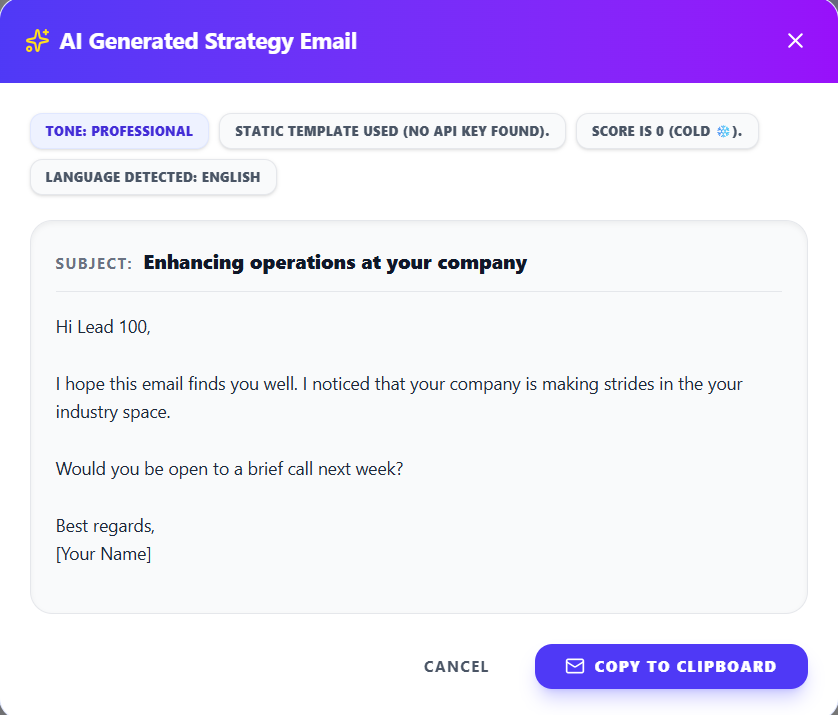
\includegraphics[width=\textwidth,height=0.82\textheight,keepaspectratio]{images/interface_ai_email.png}
    \caption{Interface de génération d'e-mails par IA}
    \label{fig:ai-email}
\end{figure}

\subsubsection{Assistant conversationnel (Chatbot) intelligent avec RAG}
Afin d'accompagner les commerciaux et managers dans leurs activités quotidiennes, nous avons développé un assistant virtuel flottant (Chatbot). Pour que cet assistant puisse répondre intelligemment et éviter les réponses génériques ou "hors-sujet", nous avons implémenté l'architecture \textbf{RAG} (Retrieval-Augmented Generation) au sein de la plateforme.

Lorsqu'un utilisateur pose une question (par exemple : \textit{"Combien avons-nous de leads qualifiés ?"} ou \textit{"Quels sont nos deals gagnés récents ?"}), le backend NestJS interroge de manière dynamique MySQL à travers Prisma pour collecter un contexte structuré (statistiques de ventes, pipeline, leads récents et tâches urgentes). Ce contexte est ensuite formaté et transmis de façon sécurisée à l'API Google Gemini (\textit{gemini-2.5-flash}) qui rédige une réponse précise, en français, et basée exclusivement sur les données réelles du CRM.

\begin{figure}[H]
    \centering
    % % \includegraphics[width=0.45\textwidth]{images/interface_chatbot.png}
    \caption{Interface de l'assistant conversationnel (Chatbot) RAG (Image manquante)}
    \label{fig:chatbot}
\end{figure}

\subsubsection{Tableau de bord Power BI}
En complément des analytiques intégrées, nous avons développé un tableau de bord Power BI connecté à la base de données MySQL. Ce dashboard offre des visualisations interactives avancées pour l'analyse des tendances de vente, la performance des commerciaux et les prévisions de revenus.

\begin{figure}[H]
    \centering
    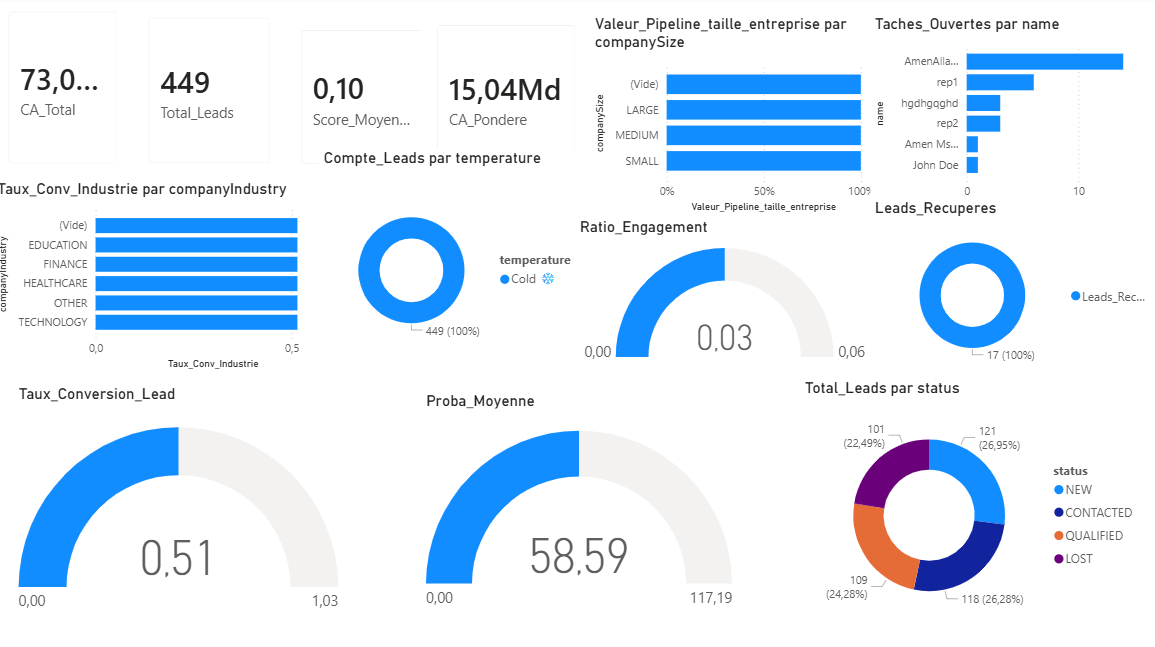
\includegraphics[width=\textwidth,height=0.82\textheight,keepaspectratio]{images/interface_powerbi1.png}
    \caption{Résumé exécutif Power BI}
    \label{fig:powerbi1}
\end{figure}

\begin{figure}[H]
    \centering
    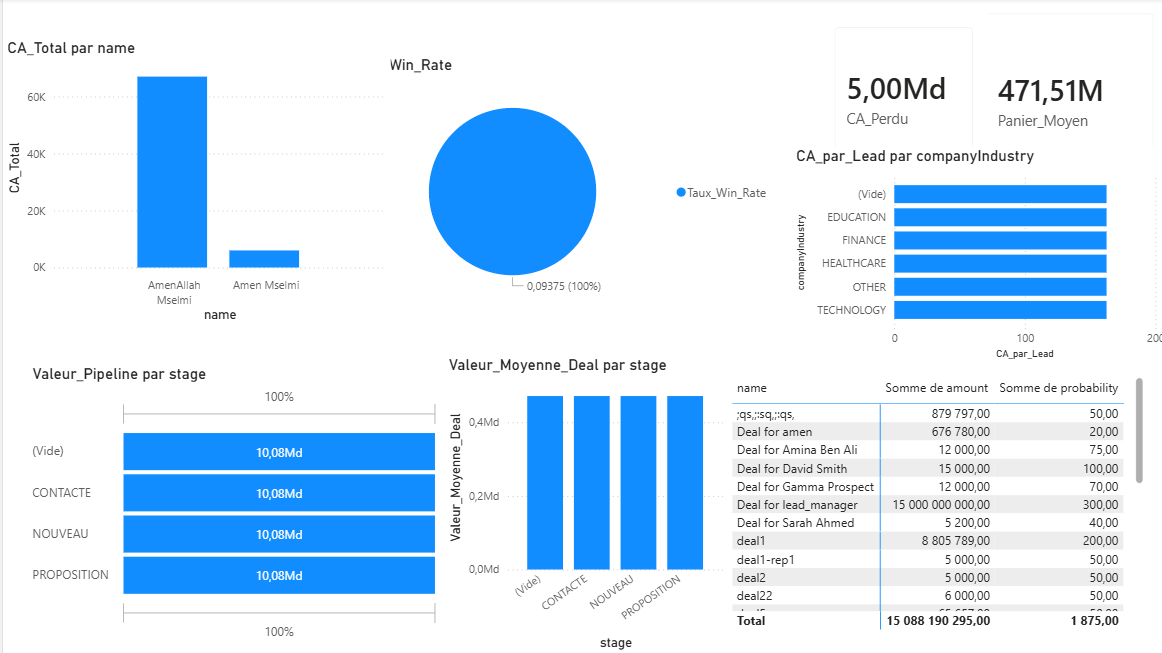
\includegraphics[width=\textwidth,height=0.82\textheight,keepaspectratio]{images/interface_powerbi2.png}
    \caption{Pipeline de ventes Power BI}
    \label{fig:powerbi2}
\end{figure}

\begin{figure}[H]
    \centering
    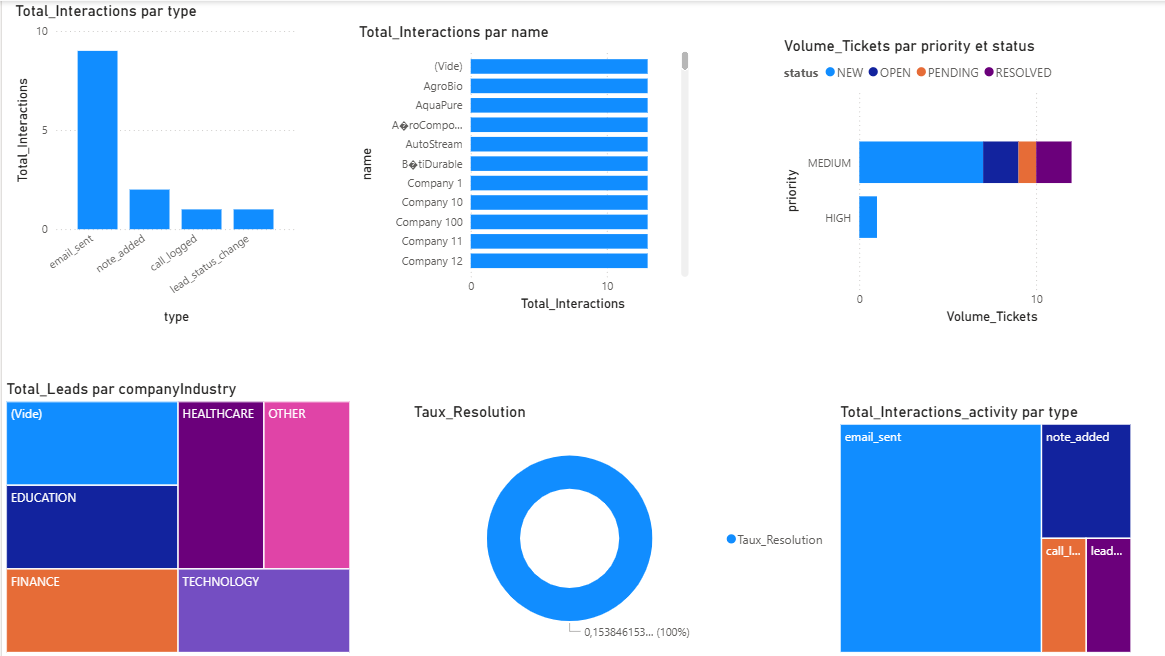
\includegraphics[width=\textwidth,height=0.82\textheight,keepaspectratio]{images/interface_powerbi3.png}
    \caption{Engagement client Power BI}
    \label{fig:powerbi3}
\end{figure}

%% ============================================================
%%  CONCLUSION
%% ============================================================
\section*{Conclusion}

Dans la phase de réalisation, nous avons utilisé des environnements techniques et logiciels spécifiques pour développer notre plateforme CRM avec scoring de leads par intelligence artificielle. Nous avons présenté notre application en illustrant ses fonctionnalités principales à travers les interfaces développées. L'architecture microservices adoptée, combinée à la conteneurisation Docker et à l'orchestration Kubernetes, assure la scalabilité et la maintenabilité de notre solution. Le pipeline CI/CD via GitHub Actions garantit un déploiement automatisé et fiable. En conclusion, nous sommes satisfaits du résultat obtenu et nous envisageons des perspectives d'amélioration pour les prochaines versions.

\clearpage

% Conclusion (page 12)
% ============================================================================
%  CONCLUSION GÉNÉRALE ET PERSPECTIVES
% ============================================================================
%  À inclure dans votre document principal avec : \input{conclusion_perspectives}
%  Pré-requis packages : hyperref, url, enumitem (normalement déjà chargés)
% ============================================================================

\chapter*{Conclusion Générale et Perspectives}
\addcontentsline{toc}{chapter}{Conclusion Générale et Perspectives}
\markboth{Conclusion Générale et Perspectives}{Conclusion Générale et Perspectives}

% ── Introduction de la conclusion ──────────────────────────────────────────────
Dans un contexte économique où l'optimisation des processus de vente et de l'écoute client constitue un levier stratégique majeur, les entreprises visent l'optimisation de leur process de vente et l'exploitation intelligente de leurs données. C'est dans cette perspective que s'inscrit notre projet de fin d'études, réalisé au sein de la société \textbf{Proxym}, portant sur la conception et le développement d'une plateforme CRM intelligente intégrant un module de \textit{Lead Scoring} basé sur l'intelligence artificielle.

% ── Récapitulatif du projet ───────────────────────────────────────────────────
Notre plateforme \textbf{CRM Lead Scoring} est conçue pour répondre aux besoins croissants des équipes commerciales en matière de gestion des prospects, de suivi des opportunités et de prise de décision assistée par les données. Des fonctionnalités telles que la gestion des leads, des contacts et des entreprises, le pipeline commercial avec suivi des deals, le système de ticketing, la messagerie interne en temps réel, les notifications, l'import CSV, la génération d'e-mails assistée par IA ainsi que l'assistant conversationnel (Chatbot) intelligent en temps réel (via Google Gemini RAG) et le scoring prédictif des leads permettent une expérience complète, intuitive et performante pour les utilisateurs. Cette approche a pour objectif d'accroître la productivité des commerciaux, d'améliorer le taux de conversion des prospects et de donner aux managers une meilleure visibilité sur l'activité de leurs équipes grâce à des tableaux de bord analytiques enrichis.

% ── Méthodologie ──────────────────────────────────────────────────────────────
C'est dans cet esprit que ce travail de fin d'études, effectué au sein de la société \textbf{Proxym}, a consisté en la conception et le développement d'une application web générique, performante, évolutive et sécurisée. Pour y parvenir, nous avons notamment choisi de nous appuyer sur la méthodologie \textbf{2TUP} (\textit{Two Track Unified Process}) fondée sur un processus de développement itératif et incrémental, permettant ainsi d'assurer une séparation nette entre les aspects fonctionnels et techniques du projet.

% ── Parcours du rapport ──────────────────────────────────────────────────────
Dans ce rapport, nous décrivons les différentes étapes que nous avons suivies pour réaliser notre solution :
\begin{itemize}
    \item Nous avons tout d'abord introduit le \textbf{cadre général} de notre travail, en précisant le contexte de l'entreprise d'accueil et la problématique traitée.
    \item Ensuite, on a présenté les \textbf{concepts clés} de la solution, notamment les architectures logicielles choisies (MVC, microservices).
    \item Nous avons précisé les autres \textbf{besoins fonctionnels et non fonctionnels} détectés ainsi que l'\textbf{analyse et spécifications des besoins} par les diagrammes de cas d'utilisation et de séquence.
    \item Puis, nous avons vu l'\textbf{aperçu conceptuel} avec les diagrammes de classes et l'architecture globale du système.
    \item Enfin, nous avons présenté la phase de \textbf{réalisation}, incluant l'environnement technique, les interfaces développées et les tests effectués.
\end{itemize}

% ── Apports du projet ────────────────────────────────────────────────────────
Il convient de noter que la réalisation de ce projet a eu des effets bénéfiques sur plusieurs plans :

\begin{itemize}
    \item \textbf{Sur le plan de la méthodologie :} Nous avons eu la chance d'apprendre les bonnes pratiques de construction grâce à la méthode \textbf{2TUP}. Cette dernière a permis une structure rigoureuse tout en offrant une souplesse face aux modifications de spécification.

    \item \textbf{En ce qui concerne la technologie :} nous avons fait usage de technologies modernes et de patterns de conception évoluées permettant d'aller bien au-delà du cadre académique. On peut citer notamment les suivantes :
    \begin{itemize}
        \item \textbf{NestJS} avec \textbf{Typescript} pour la construction d'une API RESTful, modulaire et maintenable sur la couche Backend, grâce à la mise en œuvre de la fonctionnalité des décorateurs, injection de dépendance et architecture modulaire.
        \item \textbf{Prisma ORM} et \textbf{Base de données MySQL} pour la gestion type-safe et performante de la couche persistance.
        \item \textbf{Next.js 16} et \textbf{React 19} pour le développement d'une UI réactive et moderne sur la couche Frontend, incluant la gestion du SSR et de la gestion d'état avec \textbf{Zustand}.
        \item \textbf{FastAPI} (Python) pour l'agent de scoring intelligent, basé sur un modèle de classification \textbf{Random Forest} entraîné avec \textbf{scikit-learn} pour prédire la probabilité de conversion des leads.
        \item \textbf{Socket.IO} pour la communication temps-réel (messagerie interne et notifications push).
        \item \textbf{Docker} et \textbf{Docker Compose} pour la containerisation de tous les services (MySQL, Backend, Frontend et Agent IA).
        \item \textbf{Kubernetes} et \textbf{Helm Chart} pour l'orchestration et le déploiement.
        \item \textbf{Google Gemini AI} pour la génération intelligente d'e-mails et le chatbot conversationnel avec approche RAG.
        \item \textbf{Power BI} pour la création de tableaux de bord analytiques et la visualisation des données métier.
    \end{itemize}
    
    \item \textbf{Plan personnel et professionnel :} Ce projet nous a donné une meilleure compréhension de l'impact de la profondeur du travail en équipe et de la productivité dans le cadre de l'ingénierie informatique dans une entreprise de services. Par conséquent, cette expérience nous a aidés à développer nos capacités d'intégration et de communication et la maîtrise de notre capacité de travail d'équipe, de gestion du temps et de résolution de problèmes complexes.
\end{itemize}

% ── Perspectives ─────────────────────────────────────────────────────────────
\section*{Perspectives}
\addcontentsline{toc}{section}{Perspectives}

Au sujet des perspectives futures, il est question de faire évoluer la plateforme par l'ajout de certaines fonctionnalités pouvant l'améliorer encore plus :

\begin{enumerate}
    \item \textbf{Langage naturel (NLP) :} ajouter une fonctionnalité qui peut analyser le texte d'une conversation e-mail avec un prospect pour détecter les intentions de celui-ci et son niveau de satisfaction pour un scoring plus contextuel et pertinent.

    \item \textbf{Recommandations personnalisées :} utiliser l'apprentissage machine afin de suggérer aux commerciaux des actions personnalisées comme le meilleur moment pour contacter la personne, le canal à privilégier ainsi que le contenu qu'il faut utiliser.

    \item \textbf{Analytique avancée et tableaux de bord prédictifs :} continuer la connexion de la plateforme à \textbf{Power BI} pour permettre des analyses et prévisions de vente, ainsi que des indicateurs de performance en temps réel.

    \item \textbf{Application mobile :} créer une application mobile de la plateforme soit en React Native soit en Flutter pour faciliter le travail du commercial en déplacement.

    \item \textbf{Architecture multitenant :} Adapter la plateforme afin qu'elle supporte plusieurs entreprises séparément et créer ainsi le fondement d'un modèle de service logiciel.

    \item \textbf{Évolution vers une architecture microservices :} Faire en sorte que la plateforme soit décomposée en services distincts (lead, contact, e-mails, scoring) qui s'échangent entre eux par le biais de messagerie (RabbitMQ, Kafka).

    \item \textbf{Gamification :} Intégrer des éléments de gamification (points, badges, classement) afin de motiver les équipes commerciales à utiliser la plateforme.
\end{enumerate}

% ── Clôture ──────────────────────────────────────────────────────────────────
\vspace{0.5cm}

Grâce à ce stage, nous avons donc eu le temps d'apprendre à analyser critiquement les idées pour toujours essayer de progresser et innover. Nous avons eu certaines difficultés au niveau technique notamment la configuration du pipeline CI/CD, la containerisation et le choix du modèle de Machine Learning, mais nous avons réussi à y remédier par une solution alternative. Il est important de mentionner que les contraintes de temps et de synchronisation entre les différents modules du projet ont limité nos travaux. Cependant, cette expérience nous a beaucoup apportés dans l'apprentissage rapide et la manipulation de technologies variées et complémentaires.

\vspace{0.5cm}

Finalement, nous espérons que ce modeste travail apportera satisfaction et qu'il constituera une base solide pour de futures améliorations et évolutions de la plateforme.

% ============================================================================
%  BIBLIOGRAPHIE
% ============================================================================
\begin{thebibliography}{99}

\bibitem{agile}
    Les méthodes Agiles, \textit{Nutcache}.
    \url{https://www.nutcache.com/fr/blog/les-methodes-agiles/}
    [Consulté Mai 2026].

\bibitem{2tup}
    Two Tracks Unified Process, \textit{Wikipédia}.
    \url{https://fr.wikipedia.org/wiki/Two_Tracks_Unified_Process}
    [Consulté Mai 2026].

\bibitem{processusY}
    Processus de développement en Y, \textit{SCRIBD / Blog}.
    \url{http://imilsoftware.blogspot.com/2017/01/processus-de-developpement-en-y.html}
    [Consulté Mai 2026].

\bibitem{mvc}
    MVC Architecture Pattern, \textit{Mozilla Developer Network}.
    \url{https://developer.mozilla.org/en-US/docs/Glossary/MVC}
    [Consulté Mai 2026].

\bibitem{nestjs}
    NestJS -- A progressive Node.js framework.
    \url{https://docs.nestjs.com/}
    [Consulté Mai 2026].

\bibitem{nextjs}
    Next.js Documentation, \textit{Vercel}.
    \url{https://nextjs.org/docs}
    [Consulté Mai 2026].

\bibitem{prisma}
    Prisma -- Next-generation ORM for Node.js \& TypeScript.
    \url{https://www.prisma.io/docs}
    [Consulté Mai 2026].

\bibitem{mysql}
    MySQL Documentation, \textit{Oracle}.
    \url{https://dev.mysql.com/doc/}
    [Consulté Mai 2026].

\bibitem{fastapi}
    FastAPI -- Modern Python web framework.
    \url{https://fastapi.tiangolo.com/}
    [Consulté Mai 2026].

\bibitem{sklearn}
    scikit-learn -- Machine Learning in Python.
    \url{https://scikit-learn.org/stable/}
    [Consulté Mai 2026].

\bibitem{randomforest}
    L. Breiman, ``Random Forests'', \textit{Machine Learning}, vol.~45, no.~1,
    pp.~5--32, 2001.

\bibitem{docker}
    Docker Documentation.
    \url{https://docs.docker.com/}
    [Consulté Mai 2026].

\bibitem{kubernetes}
    Kubernetes Documentation.
    \url{https://kubernetes.io/docs/}
    [Consulté Mai 2026].

\bibitem{helm}
    Helm -- The package manager for Kubernetes.
    \url{https://helm.sh/docs/}
    [Consulté Mai 2026].

\bibitem{githubactions}
    GitHub Actions Documentation.
    \url{https://docs.github.com/en/actions}
    [Consulté Mai 2026].

\bibitem{socketio}
    Socket.IO Documentation.
    \url{https://socket.io/docs/v4/}
    [Consulté Mai 2026].

\bibitem{gemini}
    Google Gemini AI API Documentation.
    \url{https://ai.google.dev/docs}
    [Consulté Mai 2026].

\bibitem{zustand}
    Zustand -- State management for React.
    \url{https://zustand-demo.pmnd.rs/}
    [Consulté Mai 2026].

\bibitem{powerbi}
    Microsoft Power BI Documentation.
    \url{https://learn.microsoft.com/en-us/power-bi/}
    [Consulté Mai 2026].

\bibitem{typescript}
    TypeScript Documentation, \textit{Microsoft}.
    \url{https://www.typescriptlang.org/docs/}
    [Consulté Mai 2026].

\bibitem{jwt}
    JSON Web Tokens -- Introduction.
    \url{https://jwt.io/introduction}
    [Consulté Mai 2026].

\end{thebibliography}
\clearpage

% ================= ANNEXES =================
% Annexes en chiffres arabes aussi
%\appendix
%\renewcommand{\chaptername}{Annexe}

% Annexe A (page 13)
%\input{annexe_a}
%\clearpage

% Annexe B (page 14)
%\input{annexe_b}
%\clearpage

% ================= BIBLIOGRAPHIE =================
% Bibliographie (page 15)
%\bibliographystyle{plain}
%\bibliography{bibliographie}
%\addcontentsline{toc}{chapter}{Bibliographie}

\end{document}